% Options for packages loaded elsewhere
\PassOptionsToPackage{unicode}{hyperref}
\PassOptionsToPackage{hyphens}{url}
%
\documentclass[
]{article}
\usepackage{amsmath,amssymb}
\usepackage{lmodern}
\usepackage{iftex}
\ifPDFTeX
  \usepackage[T1]{fontenc}
  \usepackage[utf8]{inputenc}
  \usepackage{textcomp} % provide euro and other symbols
\else % if luatex or xetex
  \usepackage{unicode-math}
  \defaultfontfeatures{Scale=MatchLowercase}
  \defaultfontfeatures[\rmfamily]{Ligatures=TeX,Scale=1}
\fi
% Use upquote if available, for straight quotes in verbatim environments
\IfFileExists{upquote.sty}{\usepackage{upquote}}{}
\IfFileExists{microtype.sty}{% use microtype if available
  \usepackage[]{microtype}
  \UseMicrotypeSet[protrusion]{basicmath} % disable protrusion for tt fonts
}{}
\makeatletter
\@ifundefined{KOMAClassName}{% if non-KOMA class
  \IfFileExists{parskip.sty}{%
    \usepackage{parskip}
  }{% else
    \setlength{\parindent}{0pt}
    \setlength{\parskip}{6pt plus 2pt minus 1pt}}
}{% if KOMA class
  \KOMAoptions{parskip=half}}
\makeatother
\usepackage{xcolor}
\usepackage[margin=1in]{geometry}
\usepackage{graphicx}
\makeatletter
\def\maxwidth{\ifdim\Gin@nat@width>\linewidth\linewidth\else\Gin@nat@width\fi}
\def\maxheight{\ifdim\Gin@nat@height>\textheight\textheight\else\Gin@nat@height\fi}
\makeatother
% Scale images if necessary, so that they will not overflow the page
% margins by default, and it is still possible to overwrite the defaults
% using explicit options in \includegraphics[width, height, ...]{}
\setkeys{Gin}{width=\maxwidth,height=\maxheight,keepaspectratio}
% Set default figure placement to htbp
\makeatletter
\def\fps@figure{htbp}
\makeatother
\setlength{\emergencystretch}{3em} % prevent overfull lines
\providecommand{\tightlist}{%
  \setlength{\itemsep}{0pt}\setlength{\parskip}{0pt}}
\setcounter{secnumdepth}{-\maxdimen} % remove section numbering
\usepackage{float} \floatplacement{figure}{H}
\usepackage{booktabs}
\usepackage{longtable}
\usepackage{array}
\usepackage{multirow}
\usepackage{wrapfig}
\usepackage{float}
\usepackage{colortbl}
\usepackage{pdflscape}
\usepackage{tabu}
\usepackage{threeparttable}
\usepackage{threeparttablex}
\usepackage[normalem]{ulem}
\usepackage{makecell}
\usepackage{xcolor}
\ifLuaTeX
  \usepackage{selnolig}  % disable illegal ligatures
\fi
\IfFileExists{bookmark.sty}{\usepackage{bookmark}}{\usepackage{hyperref}}
\IfFileExists{xurl.sty}{\usepackage{xurl}}{} % add URL line breaks if available
\urlstyle{same} % disable monospaced font for URLs
\hypersetup{
  pdftitle={Pre-assessment data-workshop for copper rockfish off California in 2023},
  pdfauthor={Dr.~Melissa Monk, Southwest Fisheries Science Center; Dr.~Chantel Wetzel, Northwest Fisheries Science Center; Dr.~Julia Coates, California Department of Fish and Wildlife},
  hidelinks,
  pdfcreator={LaTeX via pandoc}}

\title{Pre-assessment data-workshop for copper rockfish off California
in 2023}
\author{Dr.~Melissa Monk, Southwest Fisheries Science
Center \and Dr.~Chantel Wetzel, Northwest Fisheries Science
Center \and Dr.~Julia Coates, California Department of Fish and
Wildlife}
\date{2023-01-31}

\begin{document}
\maketitle

{
\setcounter{tocdepth}{3}
\tableofcontents
}
\textbf{\emph{Disclaimer: All data summaries and exploration presented
here are preliminary and may not be indicative of the final data that
will be incorporated in the 2023 assessment models}}

\hypertarget{overview}{%
\section{Overview}\label{overview}}

Description of data being considered for use in the 2023 stock
assessments for copper rockfish in California. Exploratory analyses are
provided that have been used to inform modeling choices and treatment of
data.

\hypertarget{summary-of-the-2021-assessment}{%
\section{Summary of the 2021
Assessment}\label{summary-of-the-2021-assessment}}

In 2021, copper rockfish (\emph{Sebastes caurinus}) in California waters
were modeled using two area-based models split north and south of Point
Conception. The stock status in 2021 was estimated at 18\% and 39\% of
unfished spawning output (millions of eggs) south and north of Point
Conception (\(34^\circ 27^\prime N\)), respectively.

The final assessment documents can be found online at the Pacific
Fisheries Management Council (PFMC) website:
\href{https://www.pcouncil.org/documents/2022/01/the-status-of-copper-rockfish-sebastes-caurinus-in-u-s-waters-off-the-coast-of-california-south-of-point-conception-in-2021-using-catch-and-length-data-december-2021.pdf/}{South
of Point Conception} and
\href{https://www.pcouncil.org/documents/2022/01/the-status-of-copper-rockfish-sebastes-caurinus-in-u-s-waters-off-the-coast-of-california-north-of-point-conception-in-2021-using-catch-and-length-data-december-2021.pdf/}{North
of Point Conception}

\begin{figure}
\centering
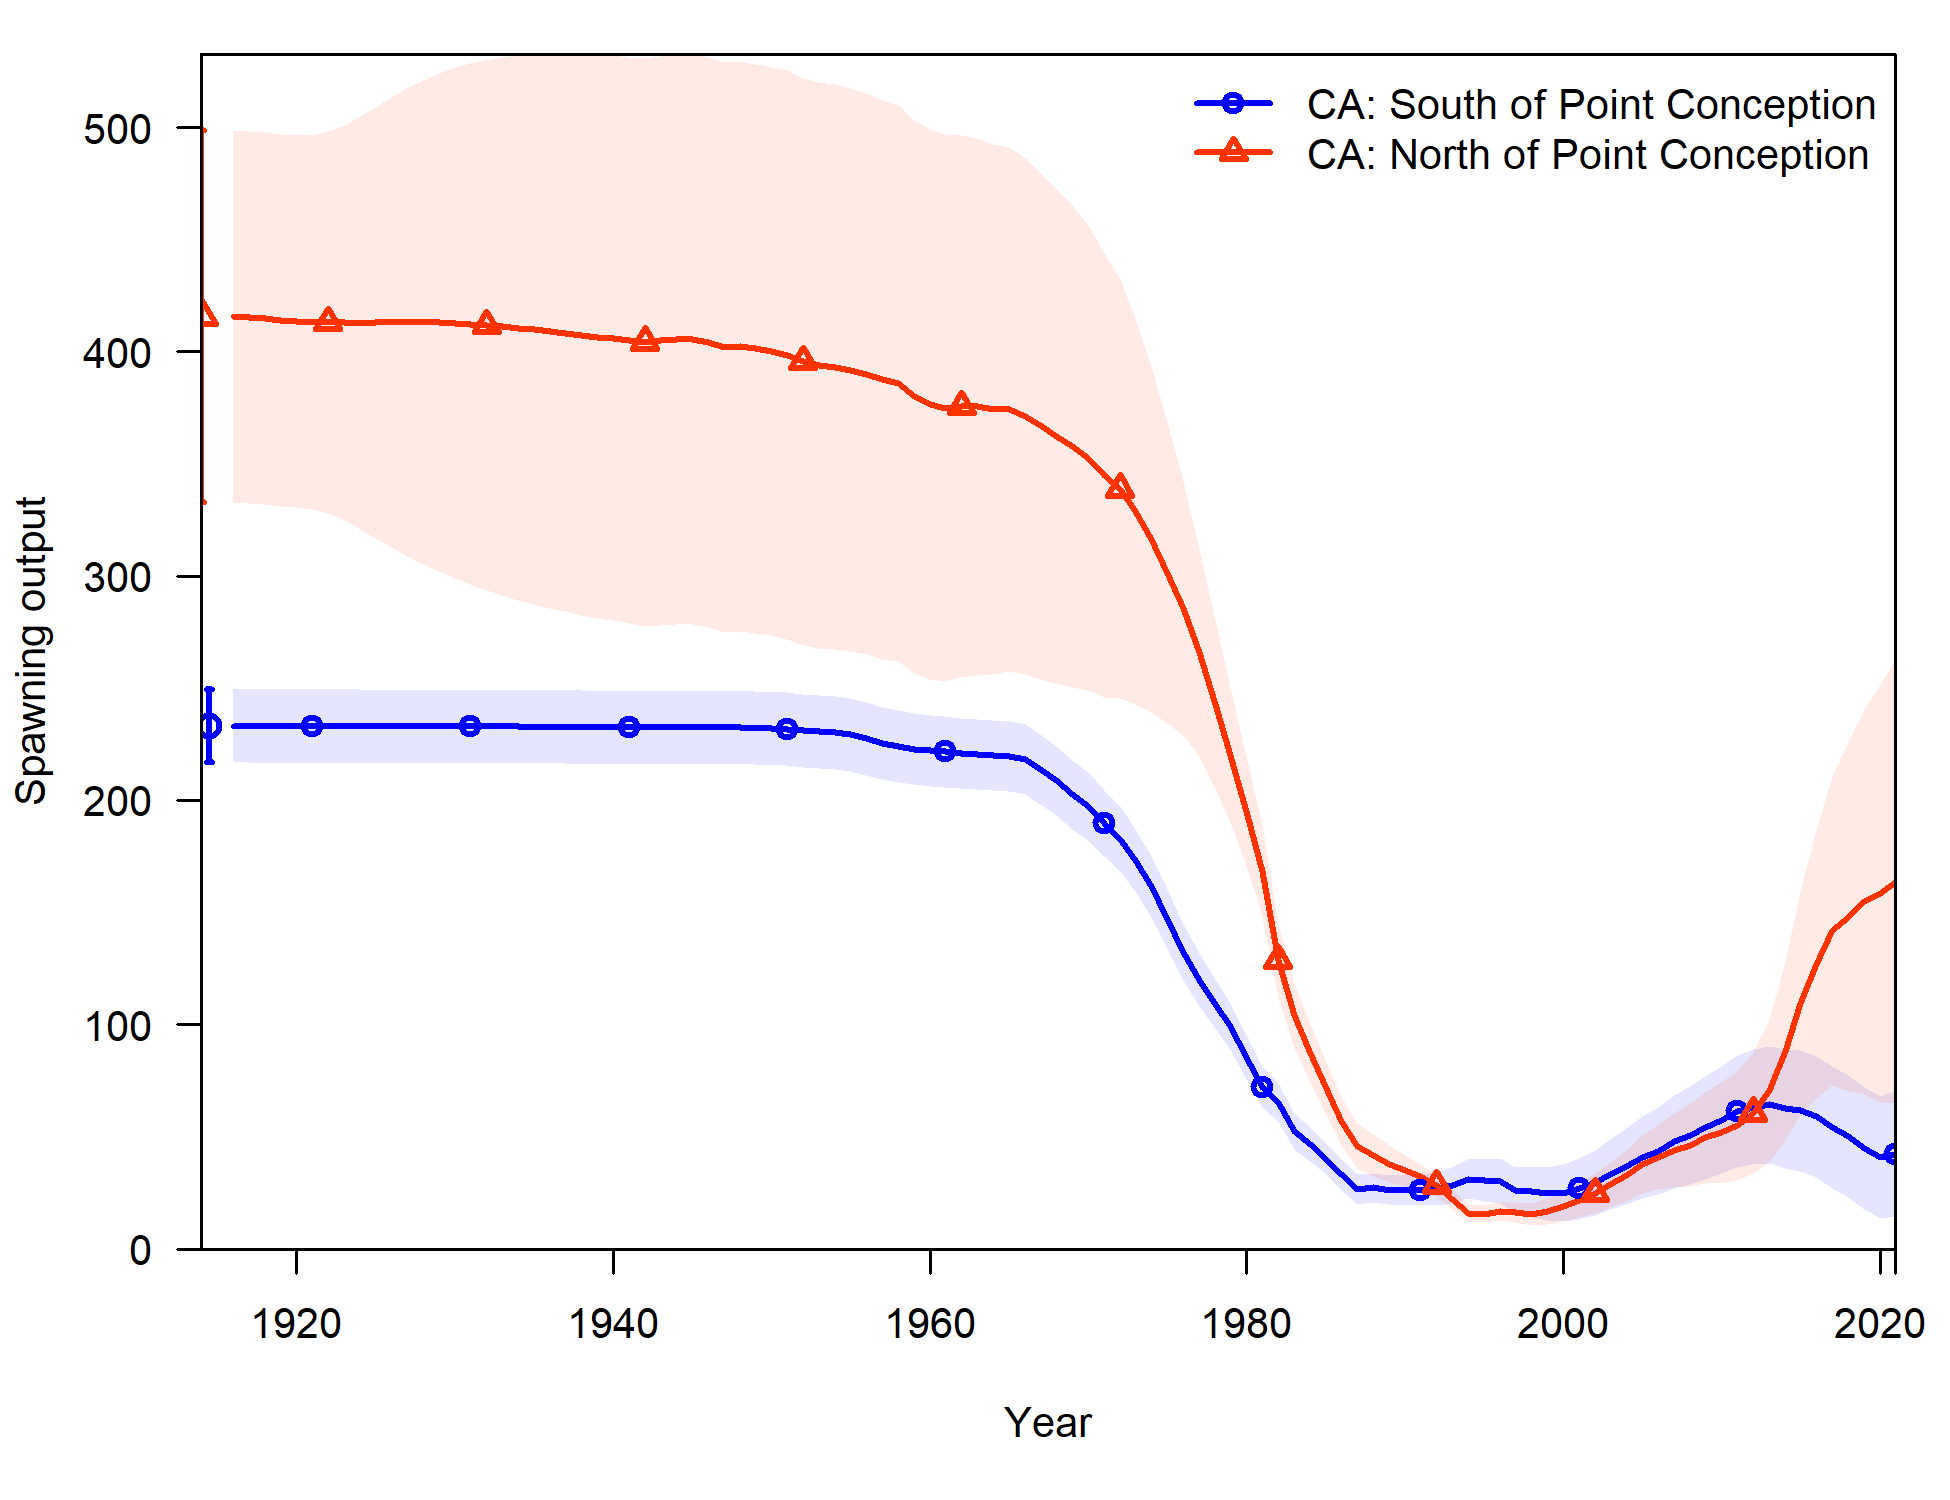
\includegraphics[width=0.75\textwidth,height=0.75\textheight]{C:/Assessments/2023/copper_rockfish_2023/docs/data_workshop/plots/ca_comprare_compare2_spawnbio_uncertainty.png}
\caption{Estimates of spawning output (millions of eggs) from each model
area in California from the 2021 data-moderate length-based
assessments.\label{fig:ssb-est}}
\end{figure}

\hypertarget{unresolved-questions-and-issues-from-the-2021-assessments}{%
\subsection{Unresolved Questions and Issues from the 2021
Assessments}\label{unresolved-questions-and-issues-from-the-2021-assessments}}

\begin{itemize}
\tightlist
\item
  Growth

  \begin{itemize}
  \tightlist
  \item
    The length-at-age relationship north of Point Conception was based
    on age and length data from Oregon and Washington due to a lack of
    age data from northern California fisheries.
  \item
    The length-at-age relationship south of Point Conception was
    informed by limited ages from the NWFSC Hook and Line and West Coast
    Groundfish Trawl surveys.
  \end{itemize}
\item
  There were additional sources of data that were not included in the
  2021 length-based data-moderate assessment that may be considered for
  use in this year's assessments:

  \begin{itemize}
  \tightlist
  \item
    Onboard Commercial Passenger Fishing Vessels (CPFV) length sample
    data from 1975-1979 (Collins and Crooke), 1987-1998 (Deb
    Wilson-Vandenberg), and 1986-1989 (Alley and Ono). These data were
    explored during mop-up and had limited impact on the model results.
  \item
    California Collaborative Fisheries Research Program (CCFRP) index of
    abundance and biological samples.
  \item
    CPFV observer index of abundance.
  \item
    RecFIN dockside sampling index of abundance.
  \item
    California Department of Fish and Wildlife (CDFW) remotely operated
    vehicle (ROV) relative of absolute biomass estimates and ROV length
    measurements.
  \item
    Any age samples from various sources that may support estimation of
    growth within the model.
  \end{itemize}
\end{itemize}

\hypertarget{potential-model-and-fleet-structure}{%
\section{Potential Model and Fleet
Structure}\label{potential-model-and-fleet-structure}}

The Stock Assessment Team (STAT) for the assessment of copper rockfish
in California waters in 2023 currently plans on retaining the same model
areas, split south and north of Point Conception, as were used in the
2021 assessments. This decision was primarily guided by the distinct
differences in the commercial and recreational fisheries seen by area.
Additionally, this approach provides the ability to easily account for
differences in biological parameters and variable recruitment success in
the two areas.

Currently, the following fleet structure is being considered for
modeling commercial and recreational fisheries in both area models:

\begin{enumerate}
\def\labelenumi{\arabic{enumi}.}
\tightlist
\item
  Commercial Passenger Fishing Vessel (CPFV, recorded as PC mode in
  RecFIN),
\item
  Private Rental (PR mode in RecFIN),
\item
  Commercial Fleet Landing Dead Fish, and
\item
  Commercial Fleet Landing Live Fish.
\end{enumerate}

Several factors have influenced the pre-preliminary fleet selection.
First, there is a differential in size of fish landed live versus dead
in the commercial fishery, particularly north of Point Conception, that
supports the need for separate selectivity curves. Second, both the CPFV
and PR recreational fleets are expected to have corresponding
fishery-dependent indices of abundance for consideration which requires
separating these recreational modes into two fleets. Finally, the
removals from the recreational man-made and beach/bank modes for copper
rockfish are very small and do not justify a separate fleet. The minimal
removals from these recreational modes will be added to the PR fleet to
account for total mortality.

The commercial lengths by year, particularly when divided into two
fleets based on the landed fish condition (live or dead), are limited in
recent years for each proposed model area. If there are issues
estimating selectivity reliably for all model years, the two commercial
fleets may be combined into a single fleet with selectivity estimated by
a parameterization that would allow bimodal selectivity (multiple peaks
in selectivity at size) using time blocks (e.g., one or more time blocks
in recent years when the live fishery developed).

Finally, each model area will have at least one fishery-independent
fleet. The CCFRP survey will be included in the model north of Point
Conception and potentially south of Point Conception depending upon the
sample sizes. For the area south of Point Conception the NWFSC Hook and
Line survey will be included as a fleet in the model.

\hypertarget{removal-data}{%
\section{Removal Data}\label{removal-data}}

\hypertarget{commerical-landings-discards}{%
\subsection{Commerical Landings \&
Discards}\label{commerical-landings-discards}}

Since 1981, landings of copper rockfish have occurred from hook and
line, net, pot, shrimp trawl, trawl, troll, and diving gear. The
majority of these landings are from hook and line gear across California
(south of Point Conception 96\% and north 87\%). North of Point
Conception there are some proportion of landings from trawl gear (8\%
primarily occurring between 1982-1985) and net gear (4\% primarily
occurring between 1983-1986). Since 2011, 98\% and 96\% of the landings
south and north of Point Conception, respectively, are coming from hook
and line gear.

In recent years, there has been an increase in the proportion of fish
landed live for both areas. In recent years, the percentage of copper
rockfish landed dead north of Point Conception has been generally less
than 50\% within each year. Fish landed live are primarily caught with
hook and line gear. However, in recent years, north of Point Conception
there have been some limited landings of live fish using pot gear.

\begin{figure}
\centering
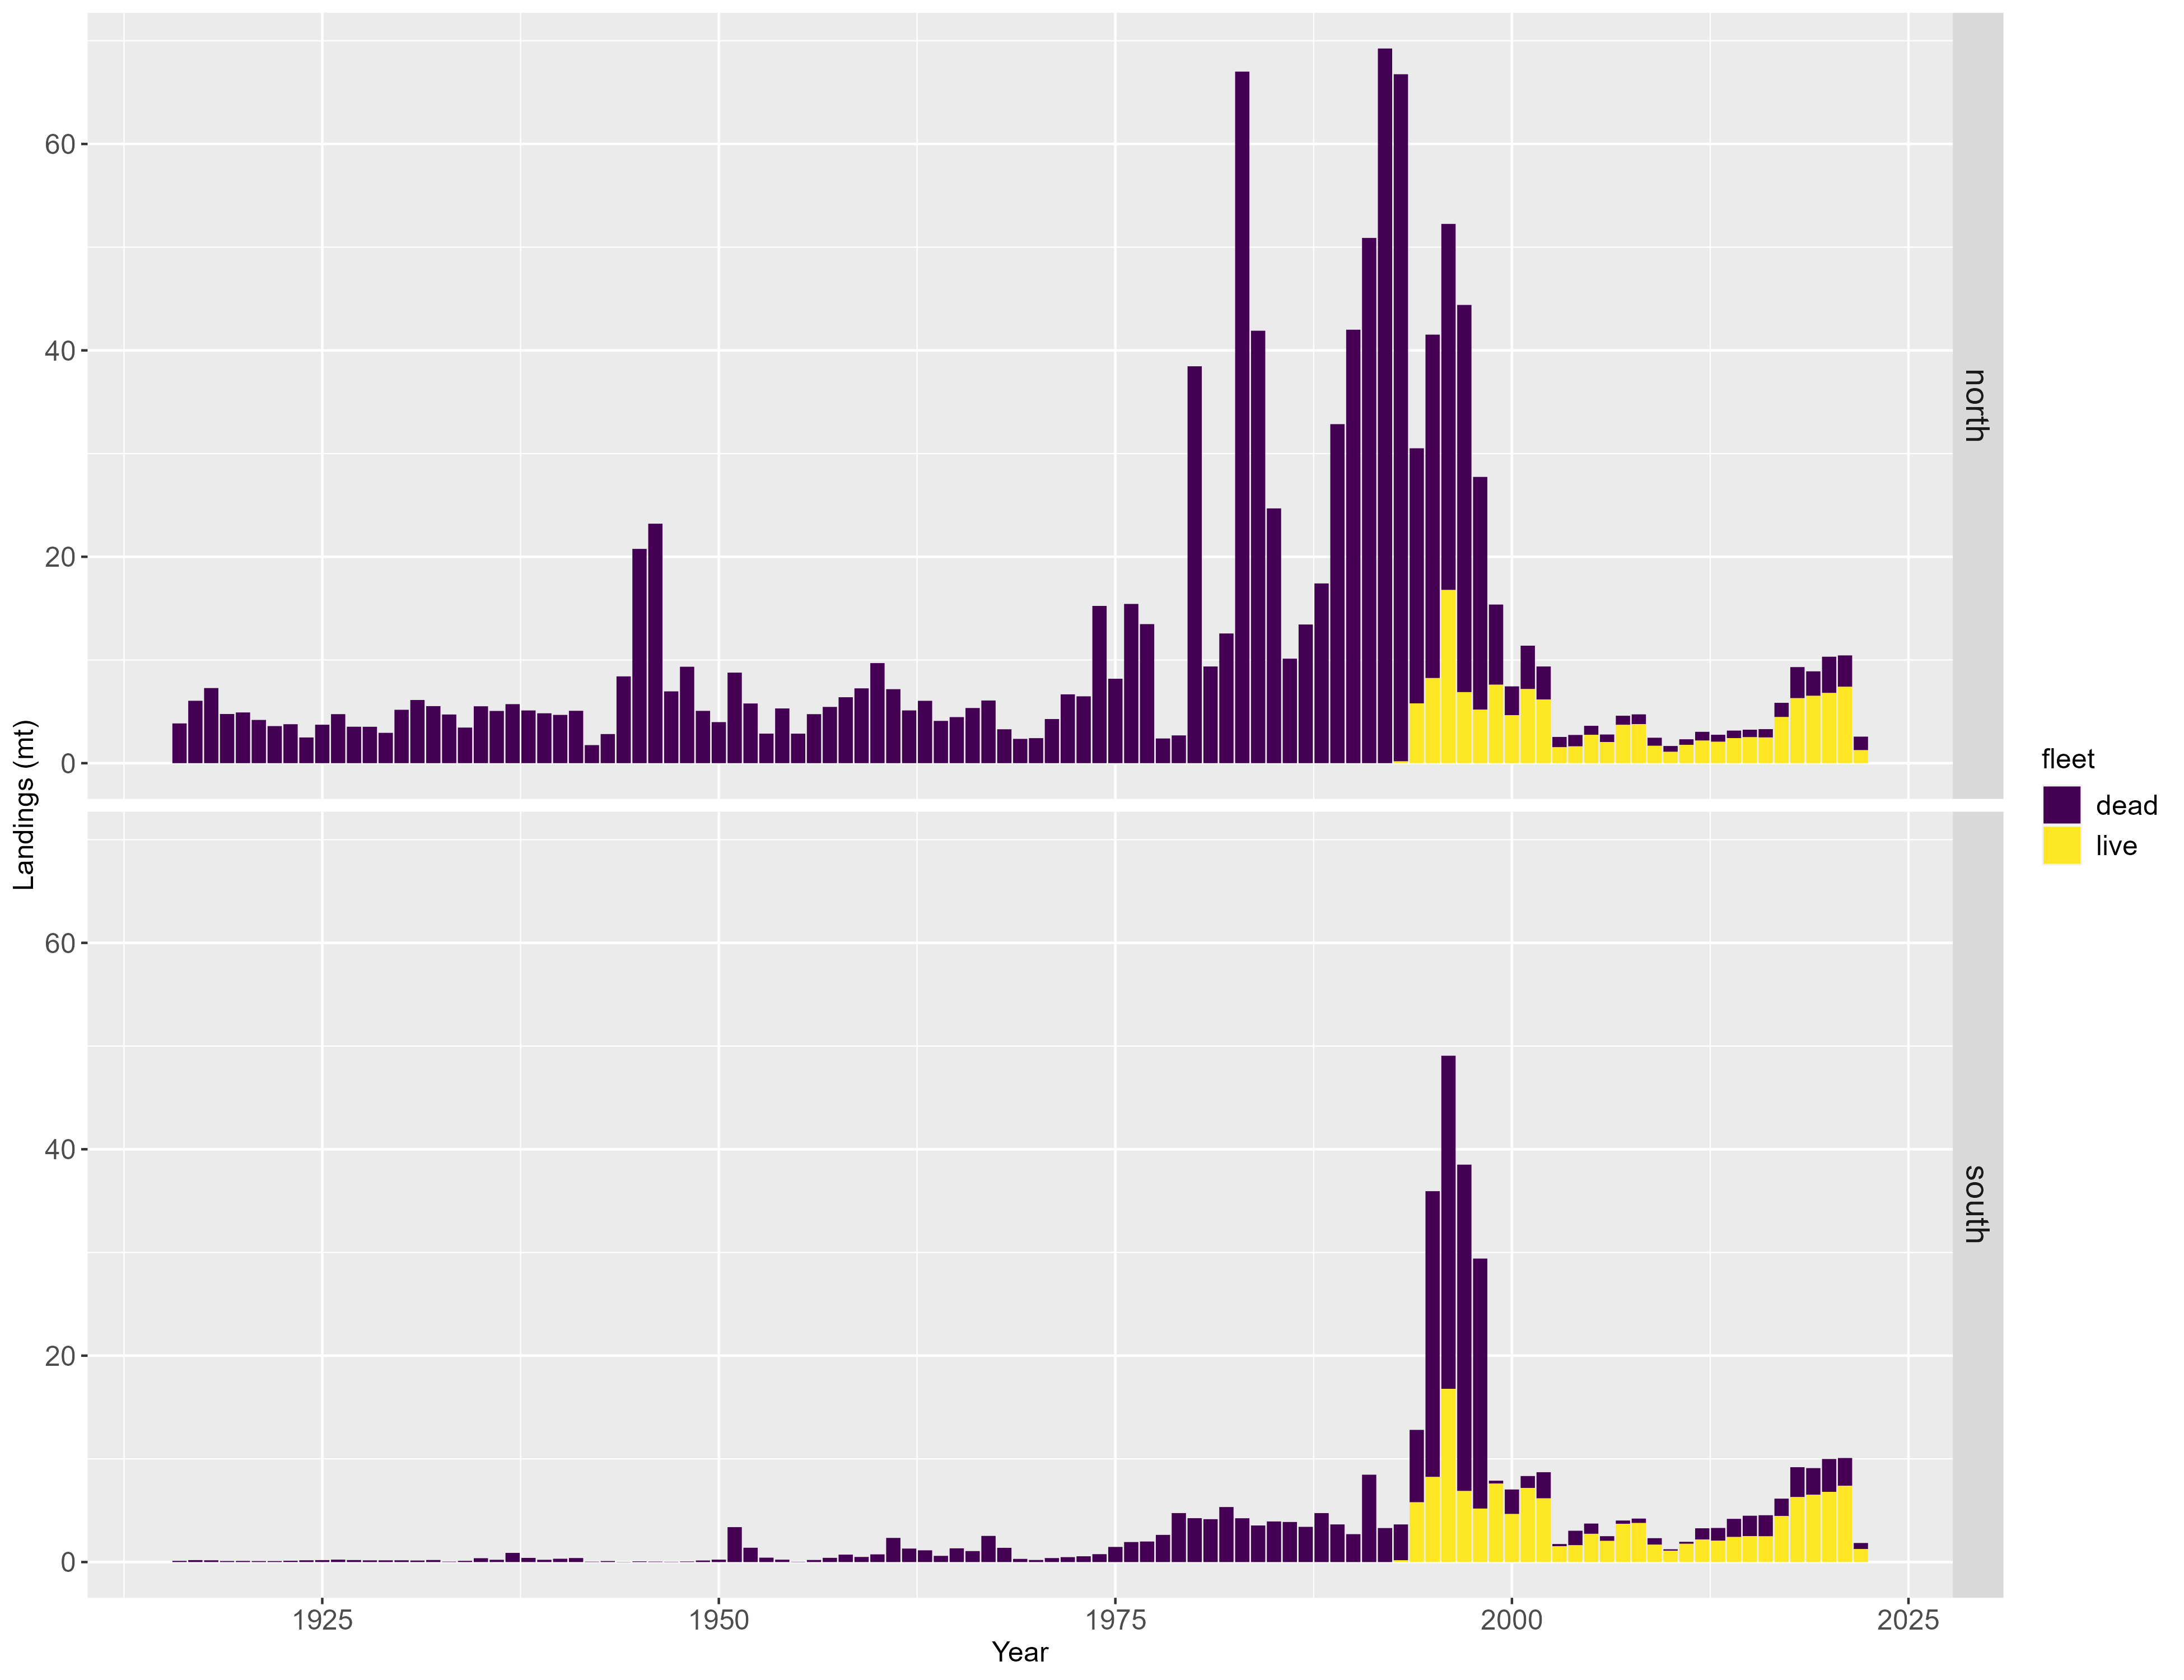
\includegraphics[width=1\textwidth,height=1\textheight]{C:/Assessments/2023/copper_rockfish_2023/docs/data_workshop/plots/landings_by_fleet_area.png}
\caption{Commercial landings north and south of Point Conception. The
landings are separated by fish landed live versus dead. The commercial
landings in the south are relatively low (less than 10 mt per year)
across the majority of years excluding 1995-1998 when landings ranged
from 24 to 32 mt. The commercial landings in the north were higher than
those observed south of Point Conception prior to 1995 with catches
peaking at 69 mt in 1994 (sources: PacFIN and California historical
catch reconstruction).\label{fig:com-landings}}
\end{figure}

\begin{figure}
\centering
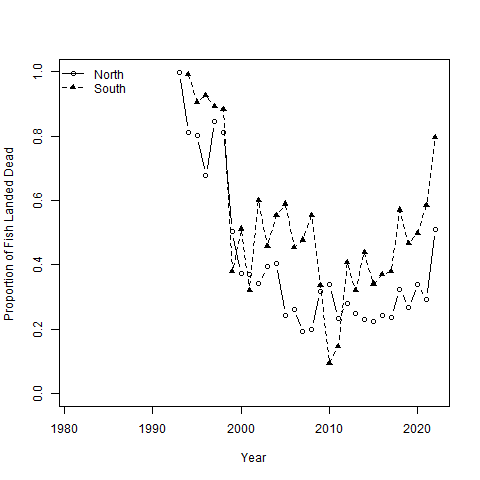
\includegraphics[width=0.75\textwidth,height=0.75\textheight]{C:/Assessments/2023/copper_rockfish_2023/docs/data_workshop/plots/percent_dead_landings.png}
\caption{Proportion of commercial landings from fish landed dead north
and south of Point Conception in recent years. The proportion lf fish
landed dead for the north are shown by a solid line with circles and the
south by a dashed line with triangles. (source:
PacFIN).\label{fig:com-prop-dead}}
\end{figure}

\begin{figure}
\centering
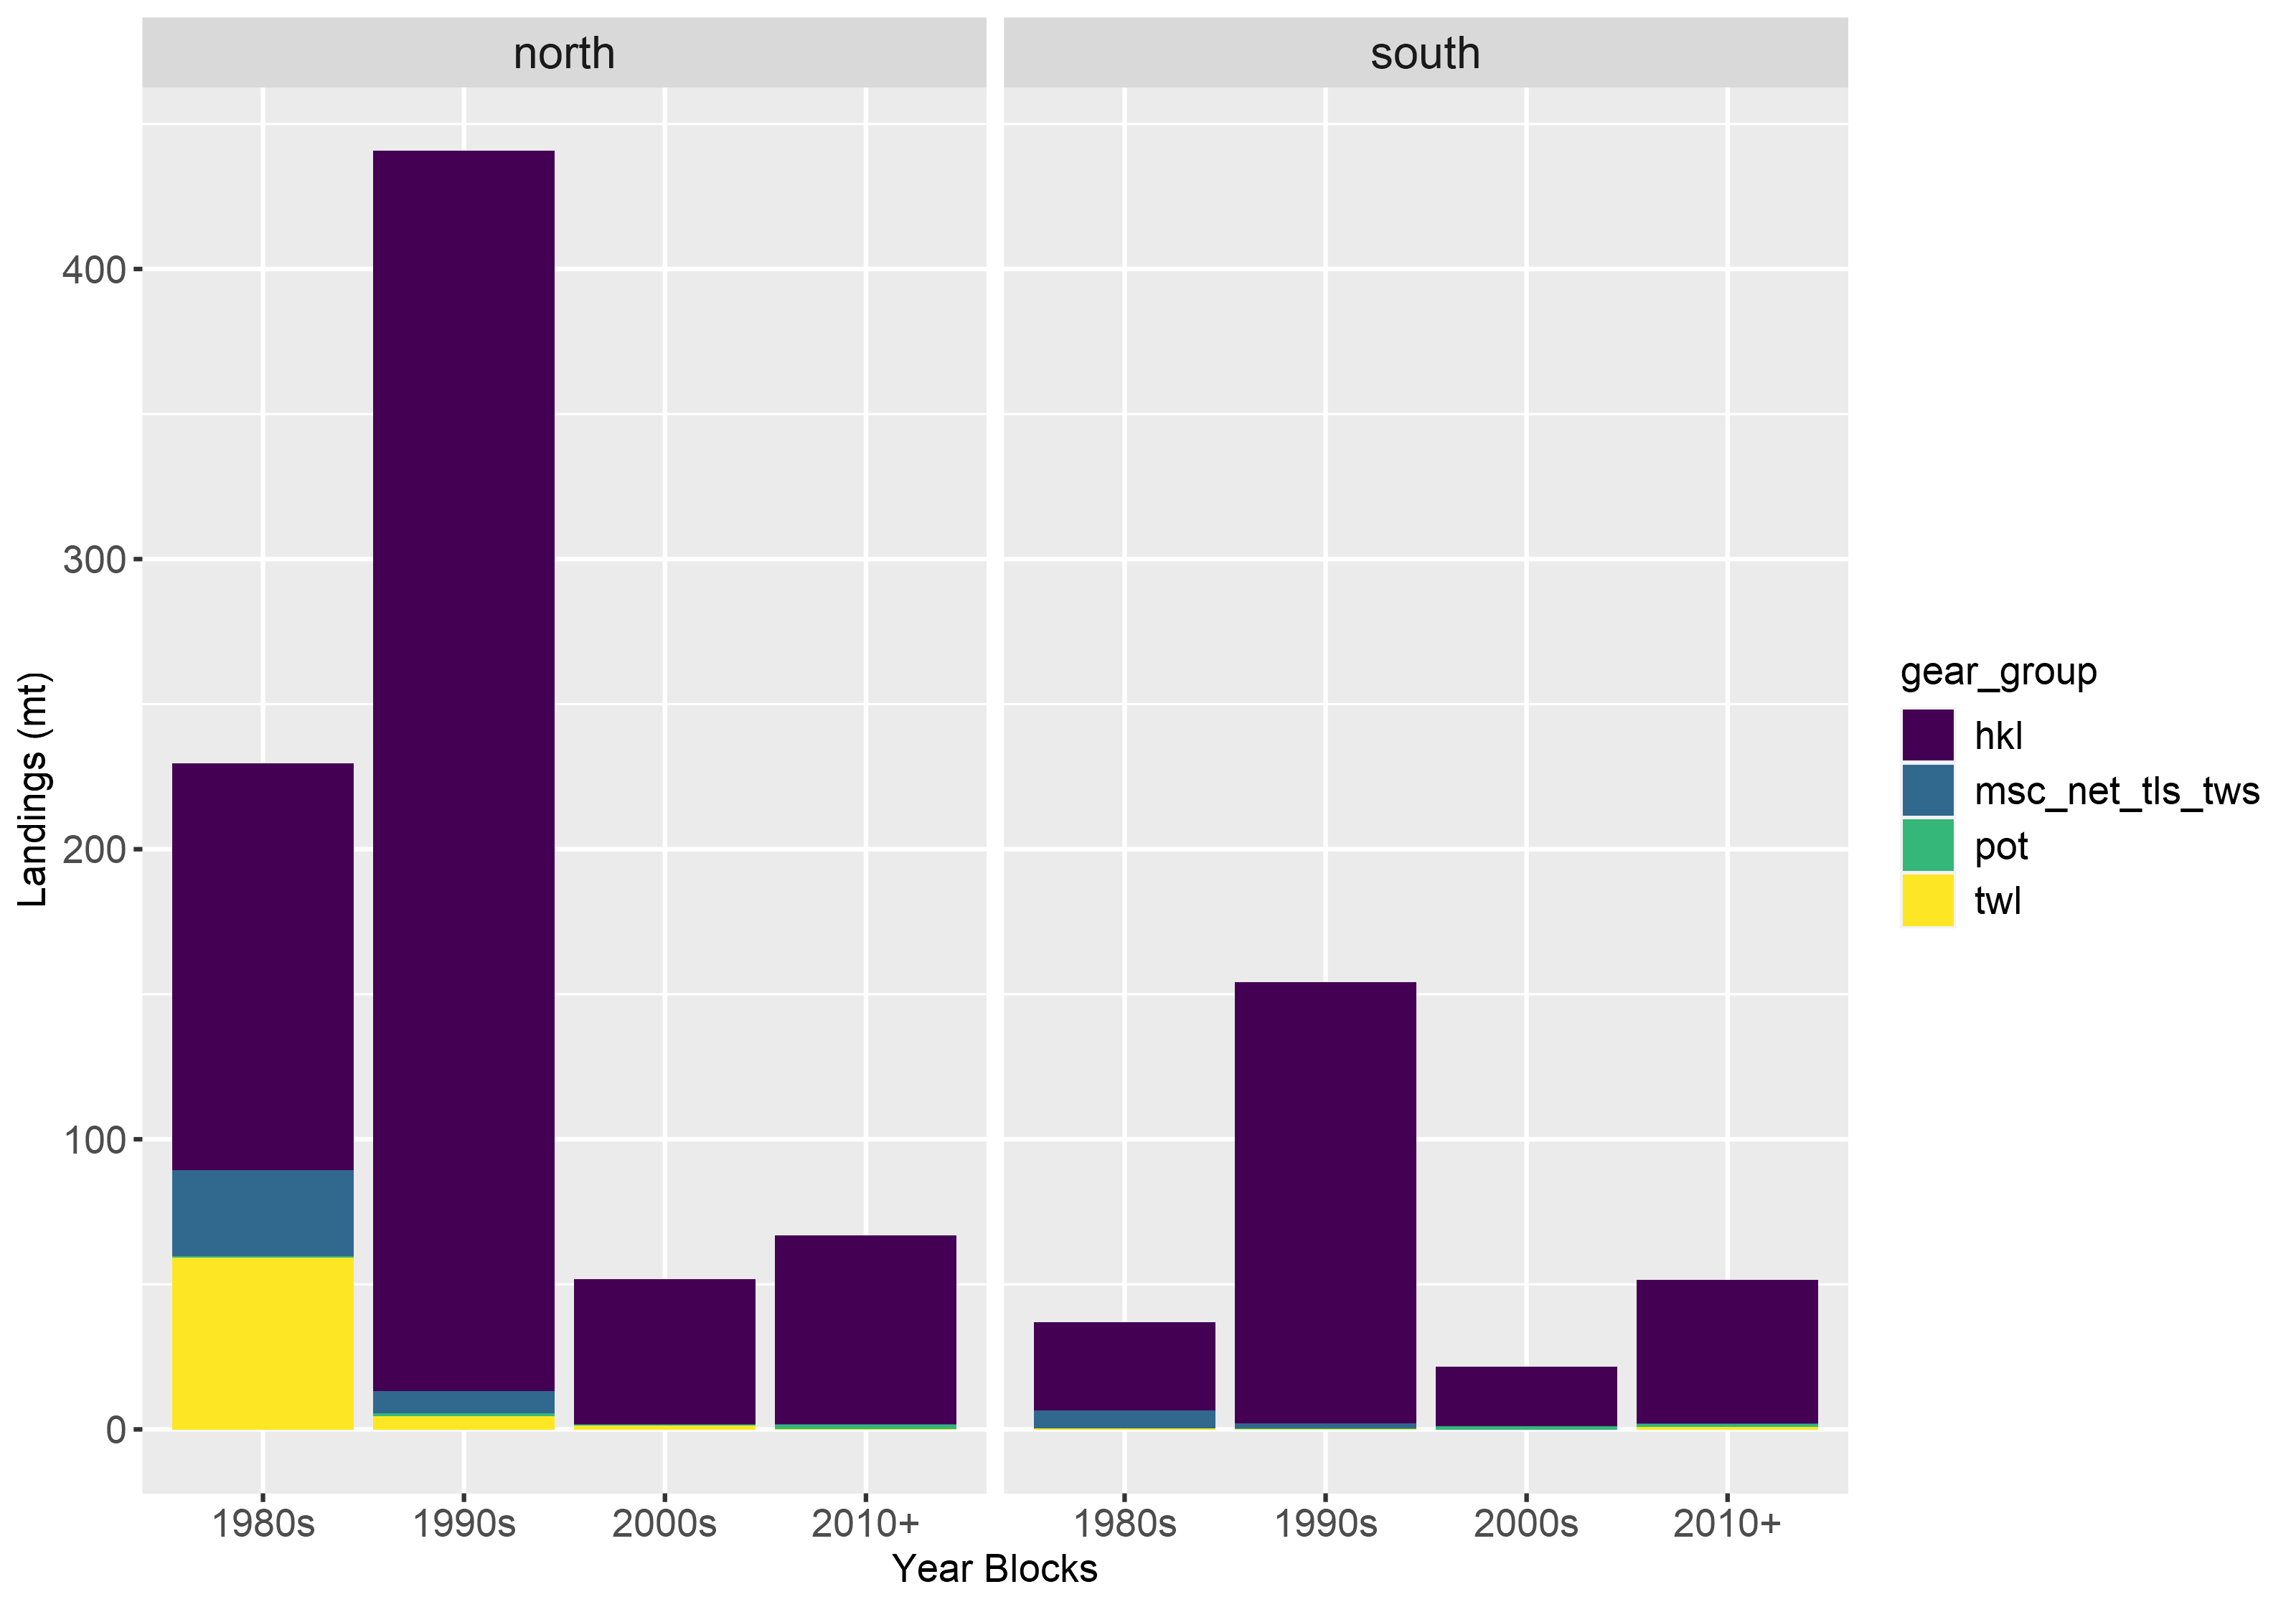
\includegraphics[width=1\textwidth,height=0.5\textheight]{C:/Assessments/2023/copper_rockfish_2023/docs/data_workshop/plots/landings_by_area_year_block_gear_group.png}
\caption{Landings by area, time period (grouped by decade), and gear
grouping: hook and line (hkl), diving gear/net/bottomfish troll/shrimp
trawl combined (msc\_net\_tls\_tws), pot, and trawl (twl) (source:
PacFIN).\label{fig:com-gear-year}}
\end{figure}

\begin{figure}
\centering
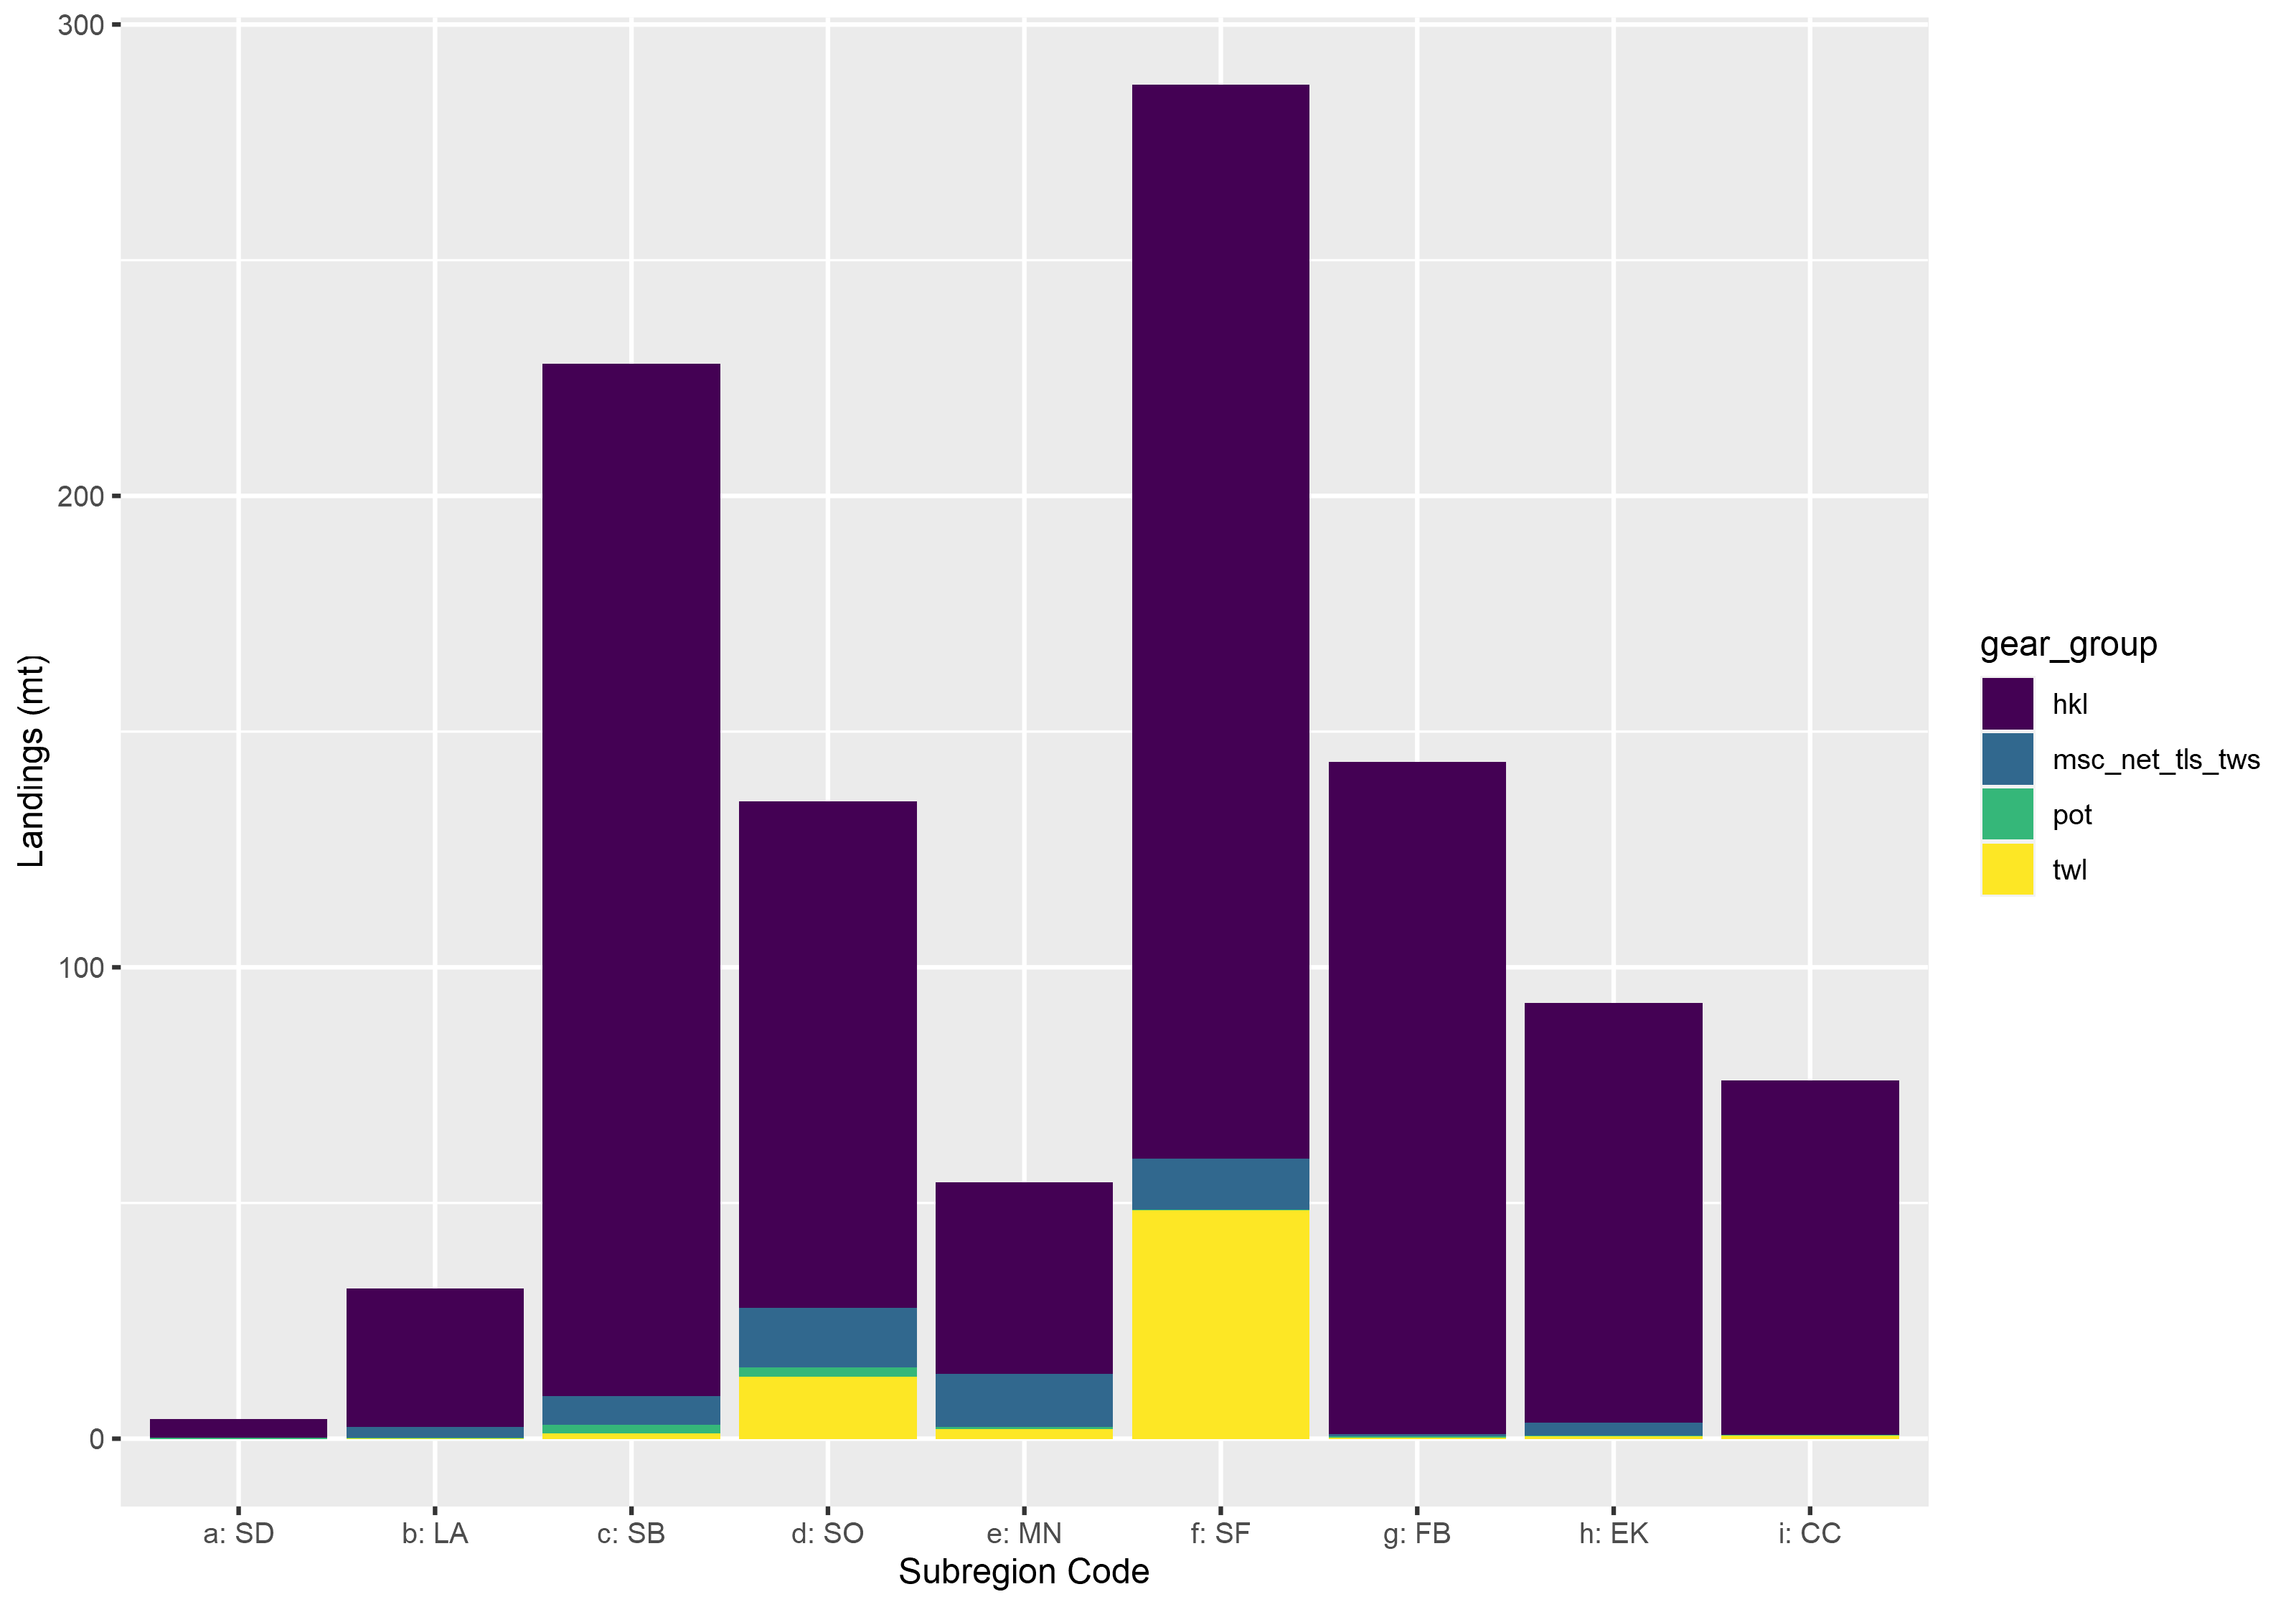
\includegraphics[width=1\textwidth,height=0.5\textheight]{C:/Assessments/2023/copper_rockfish_2023/docs/data_workshop/plots/landings_by_port_ordered_gear_group.png}
\caption{Landings by subregion and gear grouping summed across
1981-2022: hook and line (hkl), diving gear/net/bottomfish troll/shrimp
trawl combined (msc\_net\_tls\_tws), pot, and trawl (twl) (source:
PacFIN).\label{fig:com-port-gear}}
\end{figure}

\hypertarget{additional-items-for-discussion}{%
\subsubsection{Additional Items for
Discussion}\label{additional-items-for-discussion}}

Only the commercial landings are shown for each area. Discard mortality
across time will need to considered to determine catches.

\begin{itemize}
\tightlist
\item
  The 2021 assessments assumed a constant discard mortality rate of
  4.4\% informed by WCGOP data for each area in California.
\item
  The rate of discarding has likely varied across time. Are there
  particular periods of time when discarding likely increased/decreased?
\item
  Different factors impacting discarding practices by area?
\end{itemize}

\hypertarget{recreational-landings-discards}{%
\subsection{Recreational Landings \&
Discards}\label{recreational-landings-discards}}

Copper rockfish is caught by the recreational fishery across California.
Historically, landings of copper rockfish were highest in the areas
north of Point Conception. In recent years, 1993 onward, the scale of
landings of copper rockfish is similar north and south of Point
Conception. The proportion of landings by recreational modes (CPFV,
private, shoreside) across all years for each area are:

\begin{itemize}
\tightlist
\item
  North of Point Conception:

  \begin{itemize}
  \tightlist
  \item
    CPFV 34\%,
  \item
    Private = 66\%, and
  \item
    Shoreside = 0.2\%
  \end{itemize}
\item
  South of Point Conception:

  \begin{itemize}
  \tightlist
  \item
    CPFV 42\%,
  \item
    Private = 58\%, and
  \item
    Shoreside = 0\%
  \end{itemize}
\end{itemize}

However, since 1993 the CPFV fleet has accounted for 72\% of all
recreational landings south of Point Conception (only 40\% north of
Point Conception).

There are some years with missing and incomplete landings that will need
to be determined. The first gap in landings occurs due to a funding
lapse in the MRFSS program between 1990-1992. Two methods that have
commonly used in other assessments to fill in these missing data are by
averaging the landings in 1989 and 1993 and filling in the missing years
with the average or by ramping (either up or down) the landings between
1989 and 1993. Both of these approaches result in similar total landings
(the sum) for these missing years. The landings for each area prior to
and after the missing data years are:

\begin{itemize}
\tightlist
\item
  North of Point Conception

  \begin{itemize}
  \tightlist
  \item
    1989: 87 mt
  \item
    1993: 71.6 mt
  \item
    Average: 79.1 mt
  \end{itemize}
\item
  South of Point Conception

  \begin{itemize}
  \tightlist
  \item
    1989: 46.2 mt
  \item
    1993: 16.4 mt
  \item
    Average: 31.3 mt
  \end{itemize}
\end{itemize}

The landings for these missing years will be allocated by fleet based on
the proportion of landings by mode from the surrounding years.

The 2004 landings, the first years of the CRFS program, are currently
not available on RecFIN. These data were available on RecFIN in 2021 for
the previous assessments (north = 15.6 mt, south = 13.7 mt). Inquiries
have been made about the removal of these data and when the issue is
resolved the appropriate landings will be used in the 2023 assessments.

Finally, the landings from 2020 - 2021 are potentially incomplete due to
the absence of dockside sampling due to the COVID-19 pandemic. Estimates
of landings for these years have been requested from CDFW.

\begin{figure}
\centering
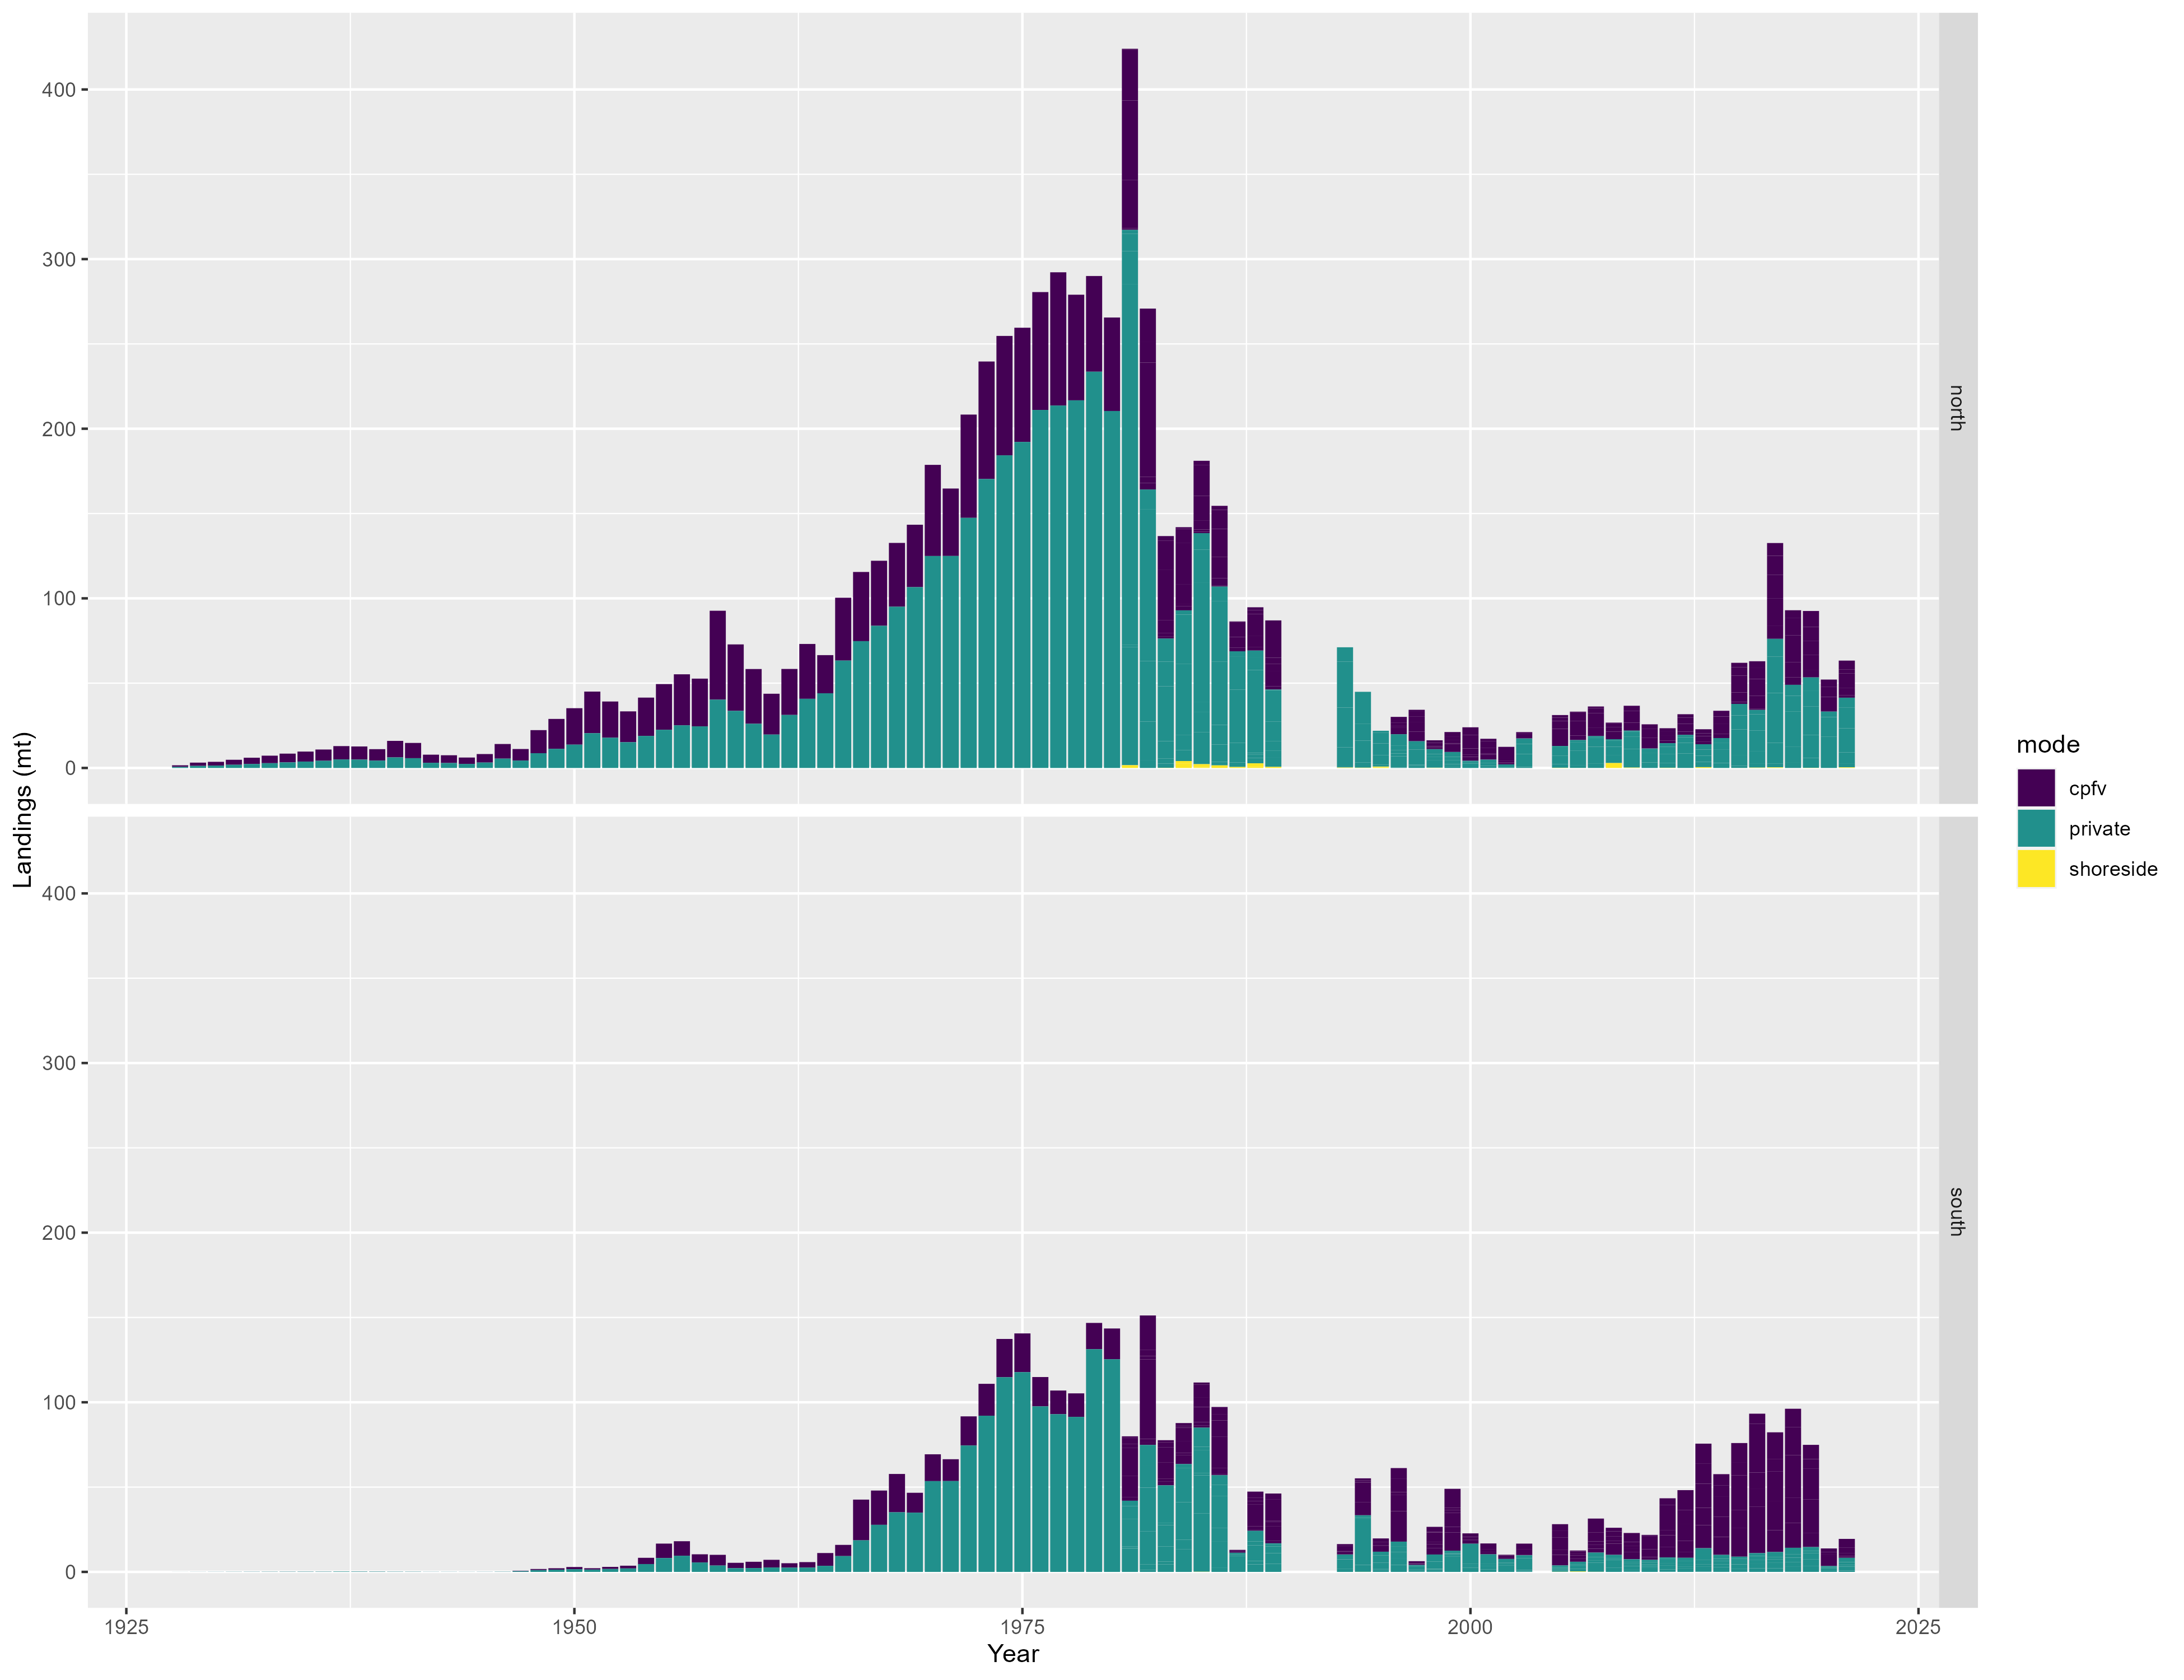
\includegraphics[width=1\textwidth,height=1\textheight]{C:/Assessments/2023/copper_rockfish_2023/docs/data_workshop/plots/all_rec_landings_mt_mode_2x1.png}
\caption{Recreational landings north and south of Point Conception
through 2021. The landings are separated by private/rental, CPFV, and
shoreside (beach and bank) modes. The landings from the CPFV fleet
predominate the recreational landings in the south since 2004. In
contrast, the majority of the removals north of Point Conception arise
from the private fleet. Landings between 1990-1992 are missing due to a
loss in fundting to MRFSS for this period. Landings from 2004 from CRFS
were not available on RecFIN. Landings in 2020 and 2021 may be
incomplete due to limited sampling during the COVID-19 pandemic and the
2022 landings were not available at the time the data were pulled.
Landings for these years will need to be determined and added (sources:
RecFIN and California historical catch
reconstruction).\label{fig:com-landings}}
\end{figure}

\begin{figure}
\centering
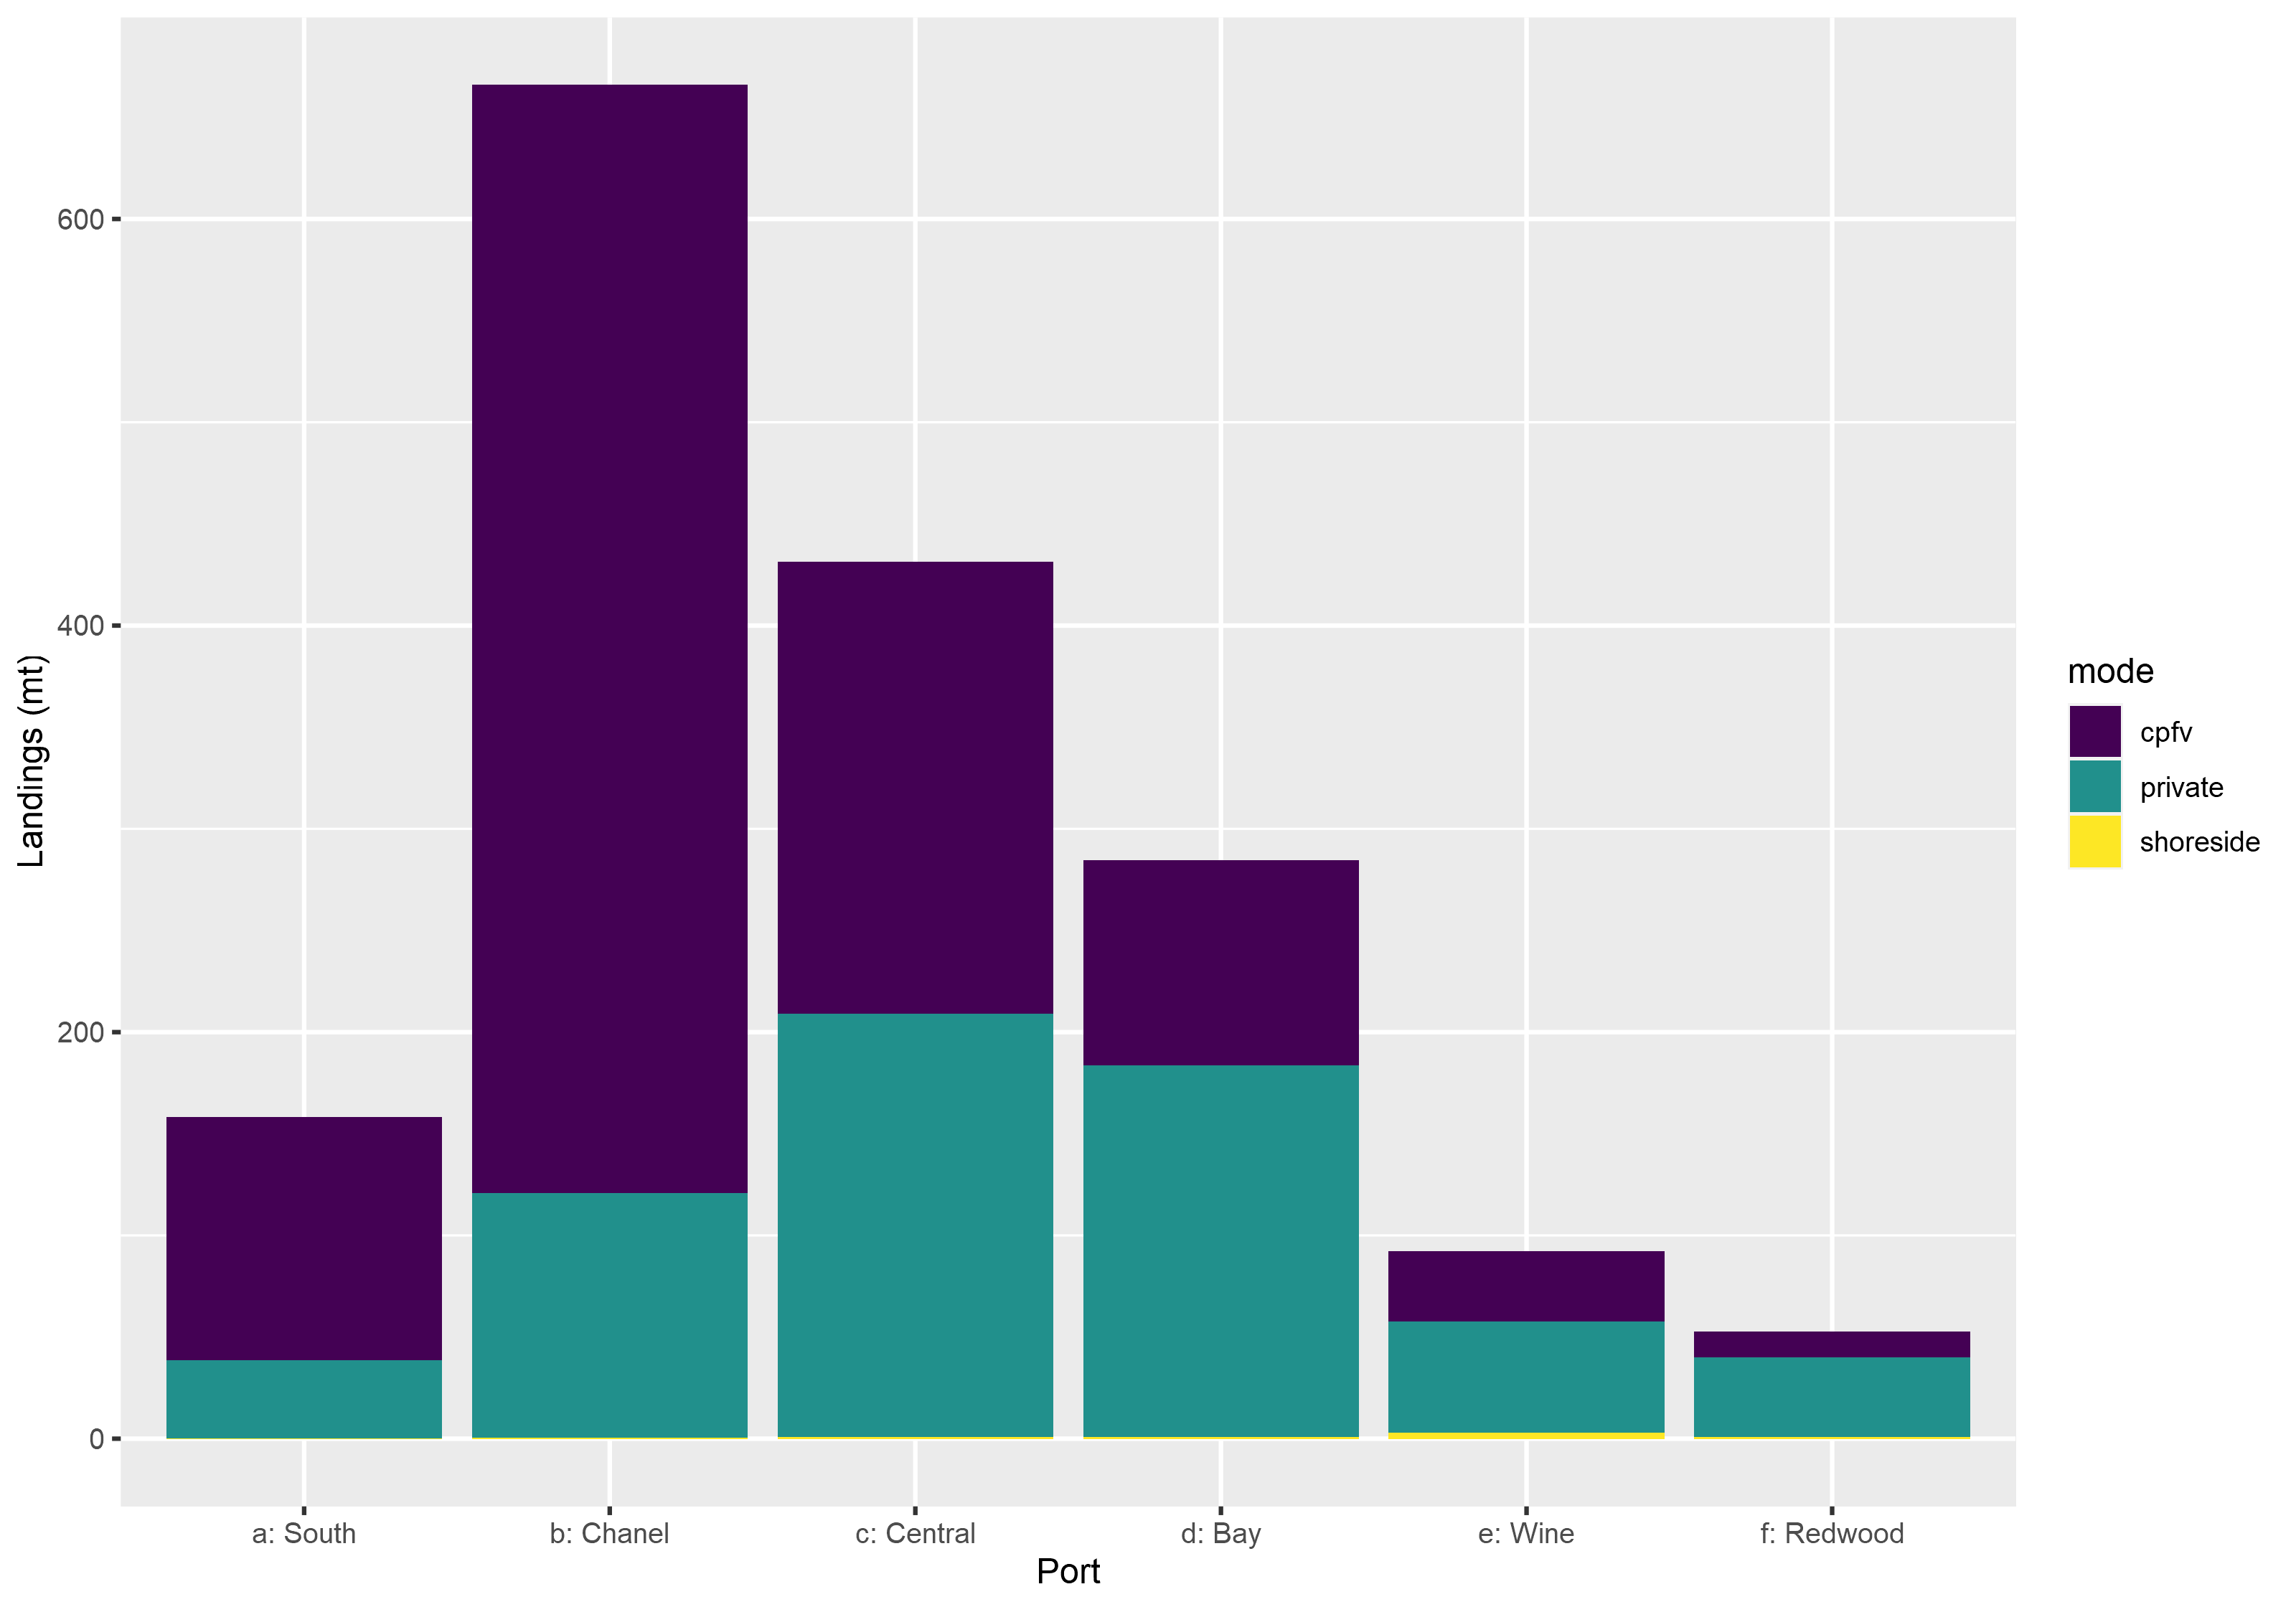
\includegraphics[width=1\textwidth,height=1\textheight]{C:/Assessments/2023/copper_rockfish_2023/docs/data_workshop/plots/crfs_landings_by_port.png}
\caption{Recreational landings in CRFS by port area and mode between
2005-2021. The landings from 2004 are currently not available in RecFIN
and the landings in 2020 and 2021 may be incomplete due to limited
sampling during the COVID-19 pandemic. Landings for these years will
need to be determined and added (source:
CRFS).\label{fig:rec-port-mode}}
\end{figure}

\hypertarget{additional-items-for-discussion-1}{%
\subsubsection{Additional Items for
Discussion}\label{additional-items-for-discussion-1}}

Only the recreational landings are shown for each area. Discard
mortality across time will need to considered to determine catches.

\begin{itemize}
\tightlist
\item
  The 2021 assessments assumed only limited discarding prior to 1981
  (0.3\% discard rate).
\item
  The rate of discarding has likely varied across time. Are there
  particular periods of time when discarding likely increased/decreased?
\item
  Different factors impacting discarding practices by area?
\end{itemize}

\hypertarget{indices-of-abundance}{%
\section{Indices of Abundance}\label{indices-of-abundance}}

\hypertarget{fishery-independent}{%
\subsection{Fishery-Independent}\label{fishery-independent}}

\hypertarget{california-cooperative-fisheries-research-program}{%
\subsubsection{California Cooperative Fisheries Research
Program}\label{california-cooperative-fisheries-research-program}}

California Collaborative Fisheries Research Program (CCFRP) is a survey
that monitors groundfish populations in California's network of Marine
Protected Areas (MPAs) and adjacent reference areas. The CCFRP survey
began in 2007 sampling select areas in northern California. In 2017,
CCFRP expanded sampling across California. A detailed summary of the
program and available sampling data for copper rockfish can be found
\href{https://www.pcouncil.org/documents/2022/05/f-3-attachment-5-california-collaborative-fisheries-research-program-data-availability-for-stock-assessments.pdf/}{online}.

Copper rockfish have been observed at every monitored MPA along the
California Coast at least once. Copper rockfish are most common at the
Carrington Point MPA in southern California, followed by the Point Lobos
and Piedras Blancas MPAs in central California.

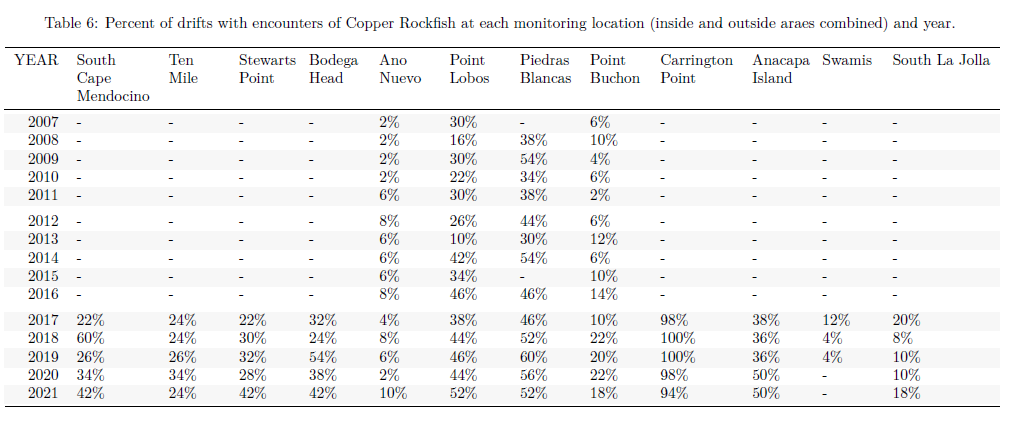
\includegraphics[width=1\textwidth,height=1\textheight]{C:/Assessments/2023/copper_rockfish_2023/docs/data_workshop/plots/ccfrp_copper_table.png}\\

\hypertarget{nwfsc-hook-and-line-survey}{%
\subsubsection{NWFSC Hook and Line
Survey}\label{nwfsc-hook-and-line-survey}}

The NWFSC Hook and Line survey begun sampling shelf rockfish over rocky
reef habitat within the Southern California Bight in 2004 using rod and
reel gear. Since, 2005, sampling has been conducted in late-September
through early-October. The minimum and maximum sampling depths are set
at 20 fathoms (37 meters) to 141 fathoms (257 meters). Starting in 2014,
the survey added sampling sites with the Cowcod Conservation Area (CCA).
The depth of sites sampled within the CCA range between 25 - 128 fathoms
and the depth of sites sampled outside the CCA range between 20 -141
fathoms.

Between 2004-2021 the NWFSC Hook and Line survey has caught a total of
1,151 copper rockfish. The majority of these observations have occurred
outside the CCA (outside CCA = 1,057 and inside CCA = 94). The NWFSC
Hook and Line data from 2022 is not yet available and not included in
these data summaries.

\begin{figure}
\centering
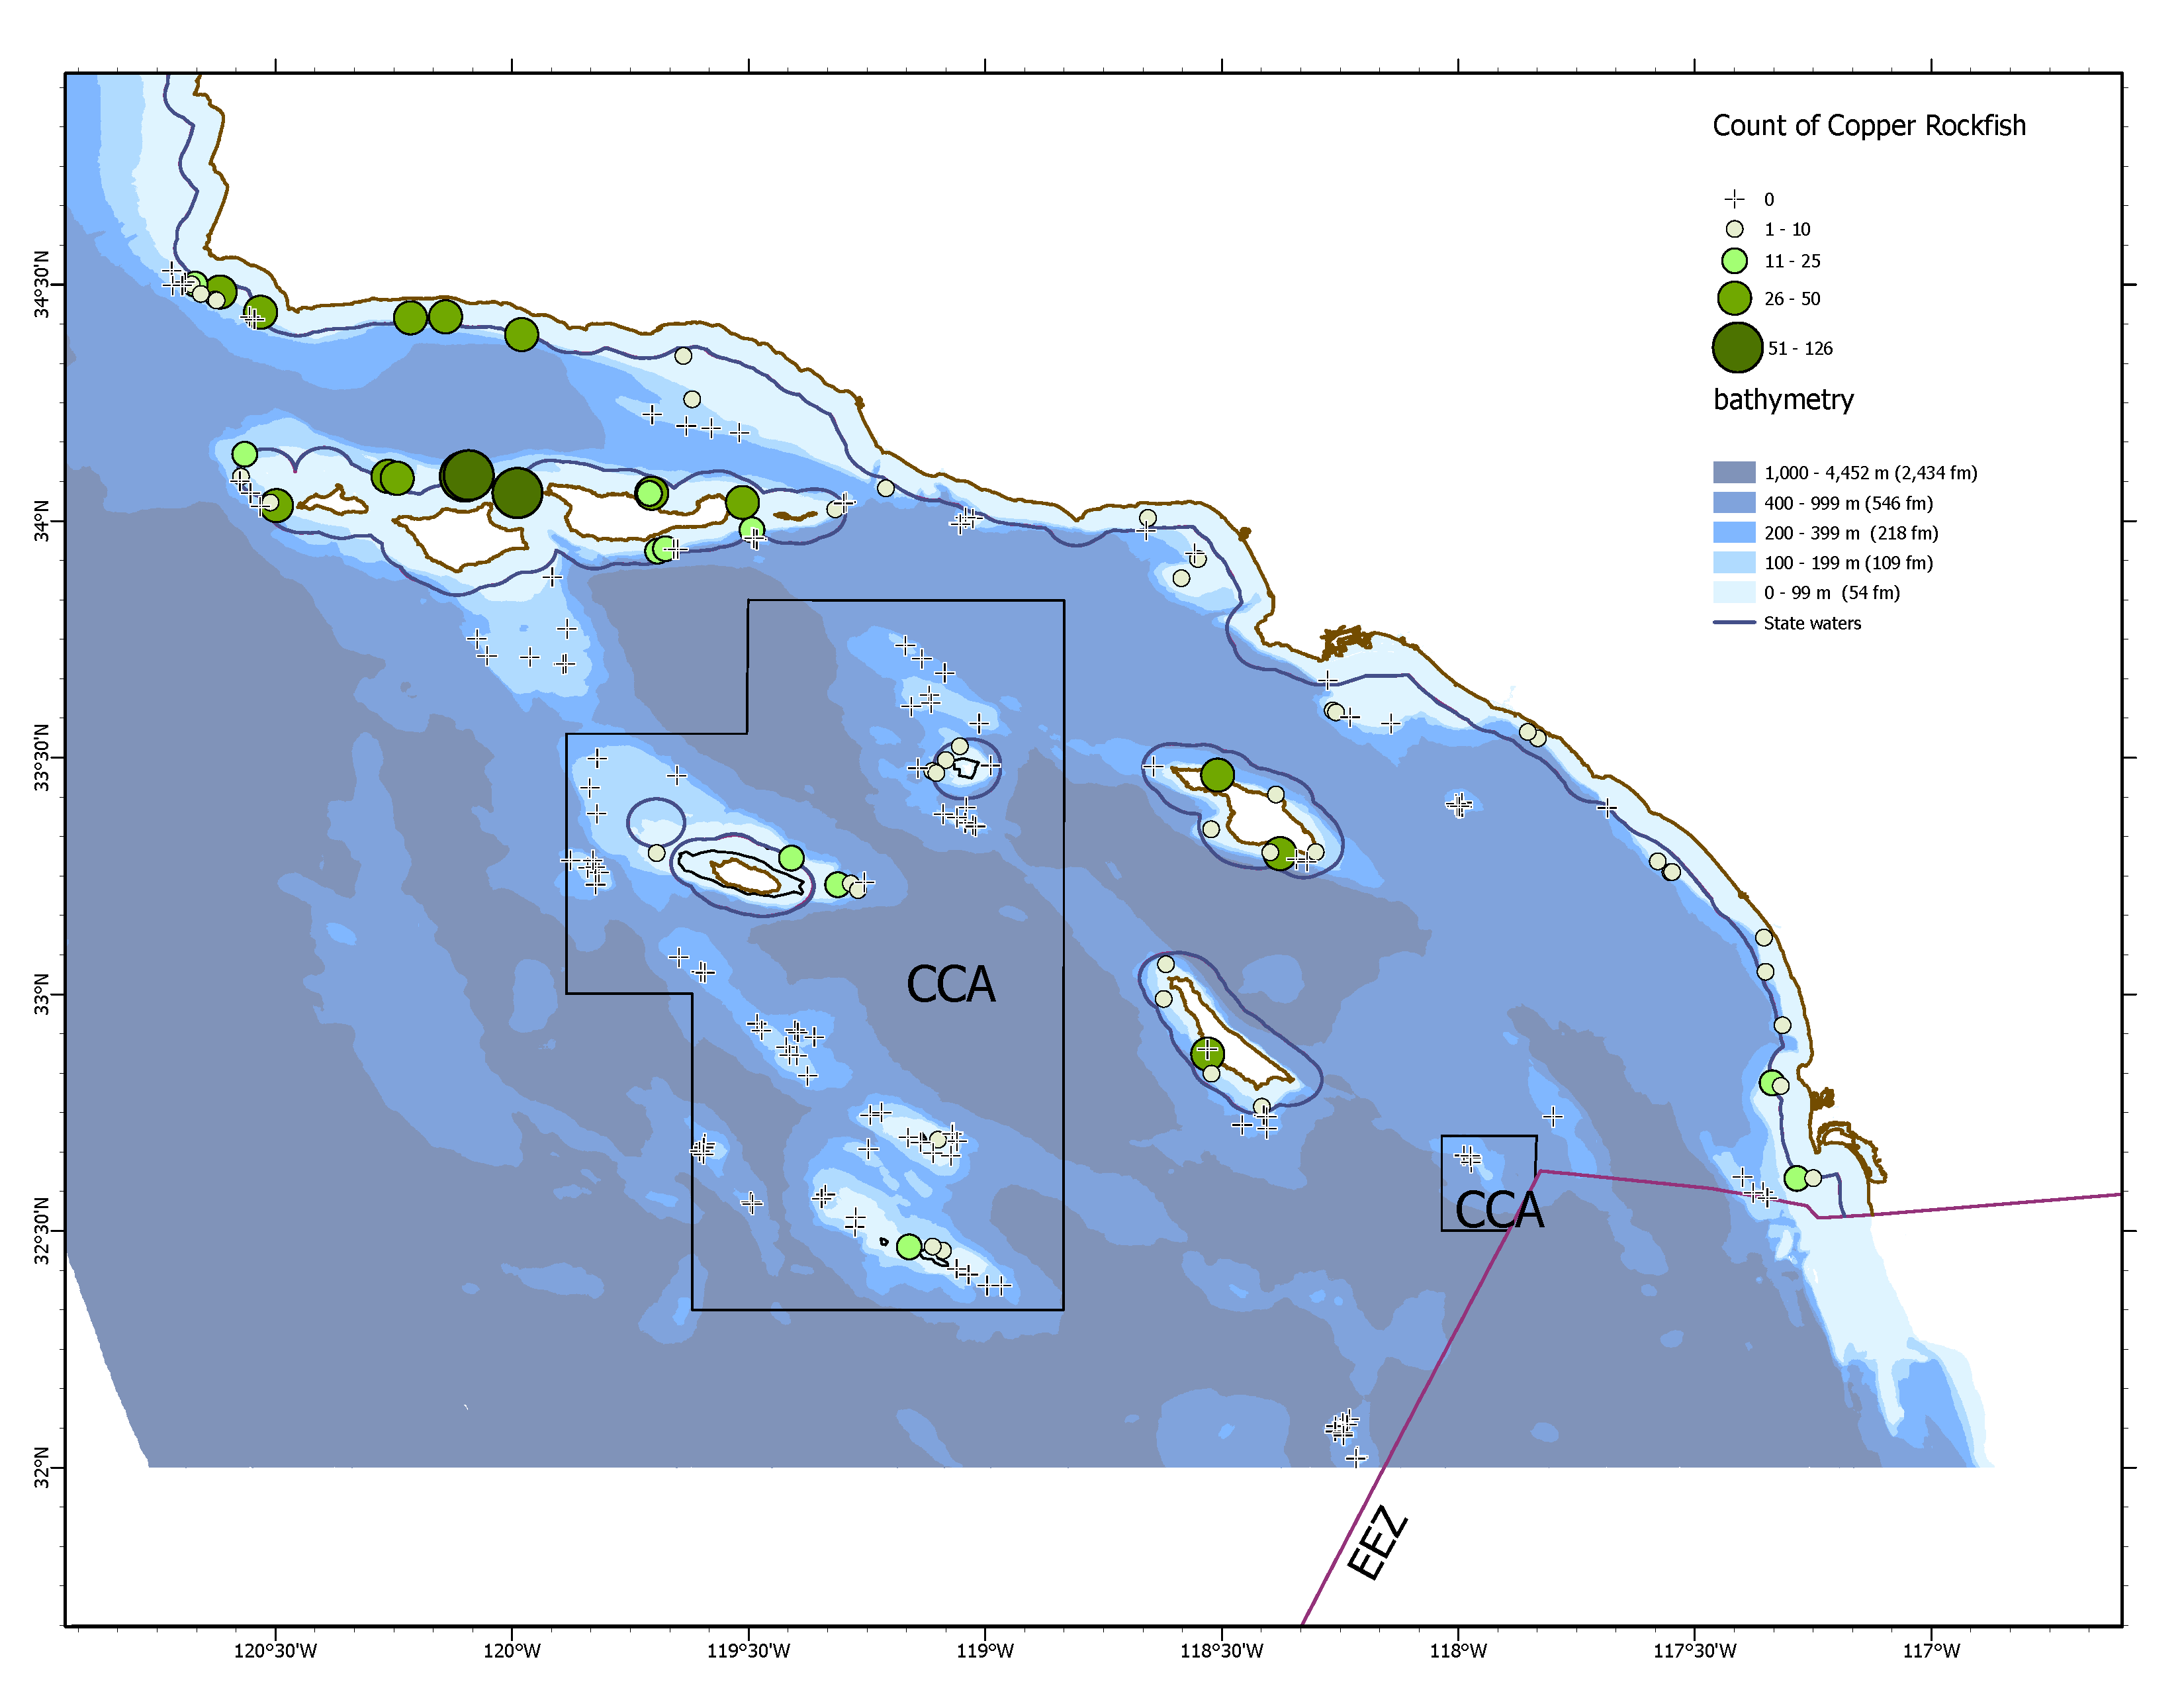
\includegraphics[width=1\textwidth,height=1\textheight]{C:/Assessments/2023/copper_rockfish_2023/docs/data_workshop/plots/hkl_copper_by_site_count.png}
\caption{Total number of observation of copper rockfish between
2004-2021 by sampling site inside and outside of Cowcod Conservation
Areas (CCA) from the NWFSC Hook and Line survey (source: NWFSC Hook and
Line survey).\label{fig:hkl-sites}}
\end{figure}

\begin{figure}
\centering
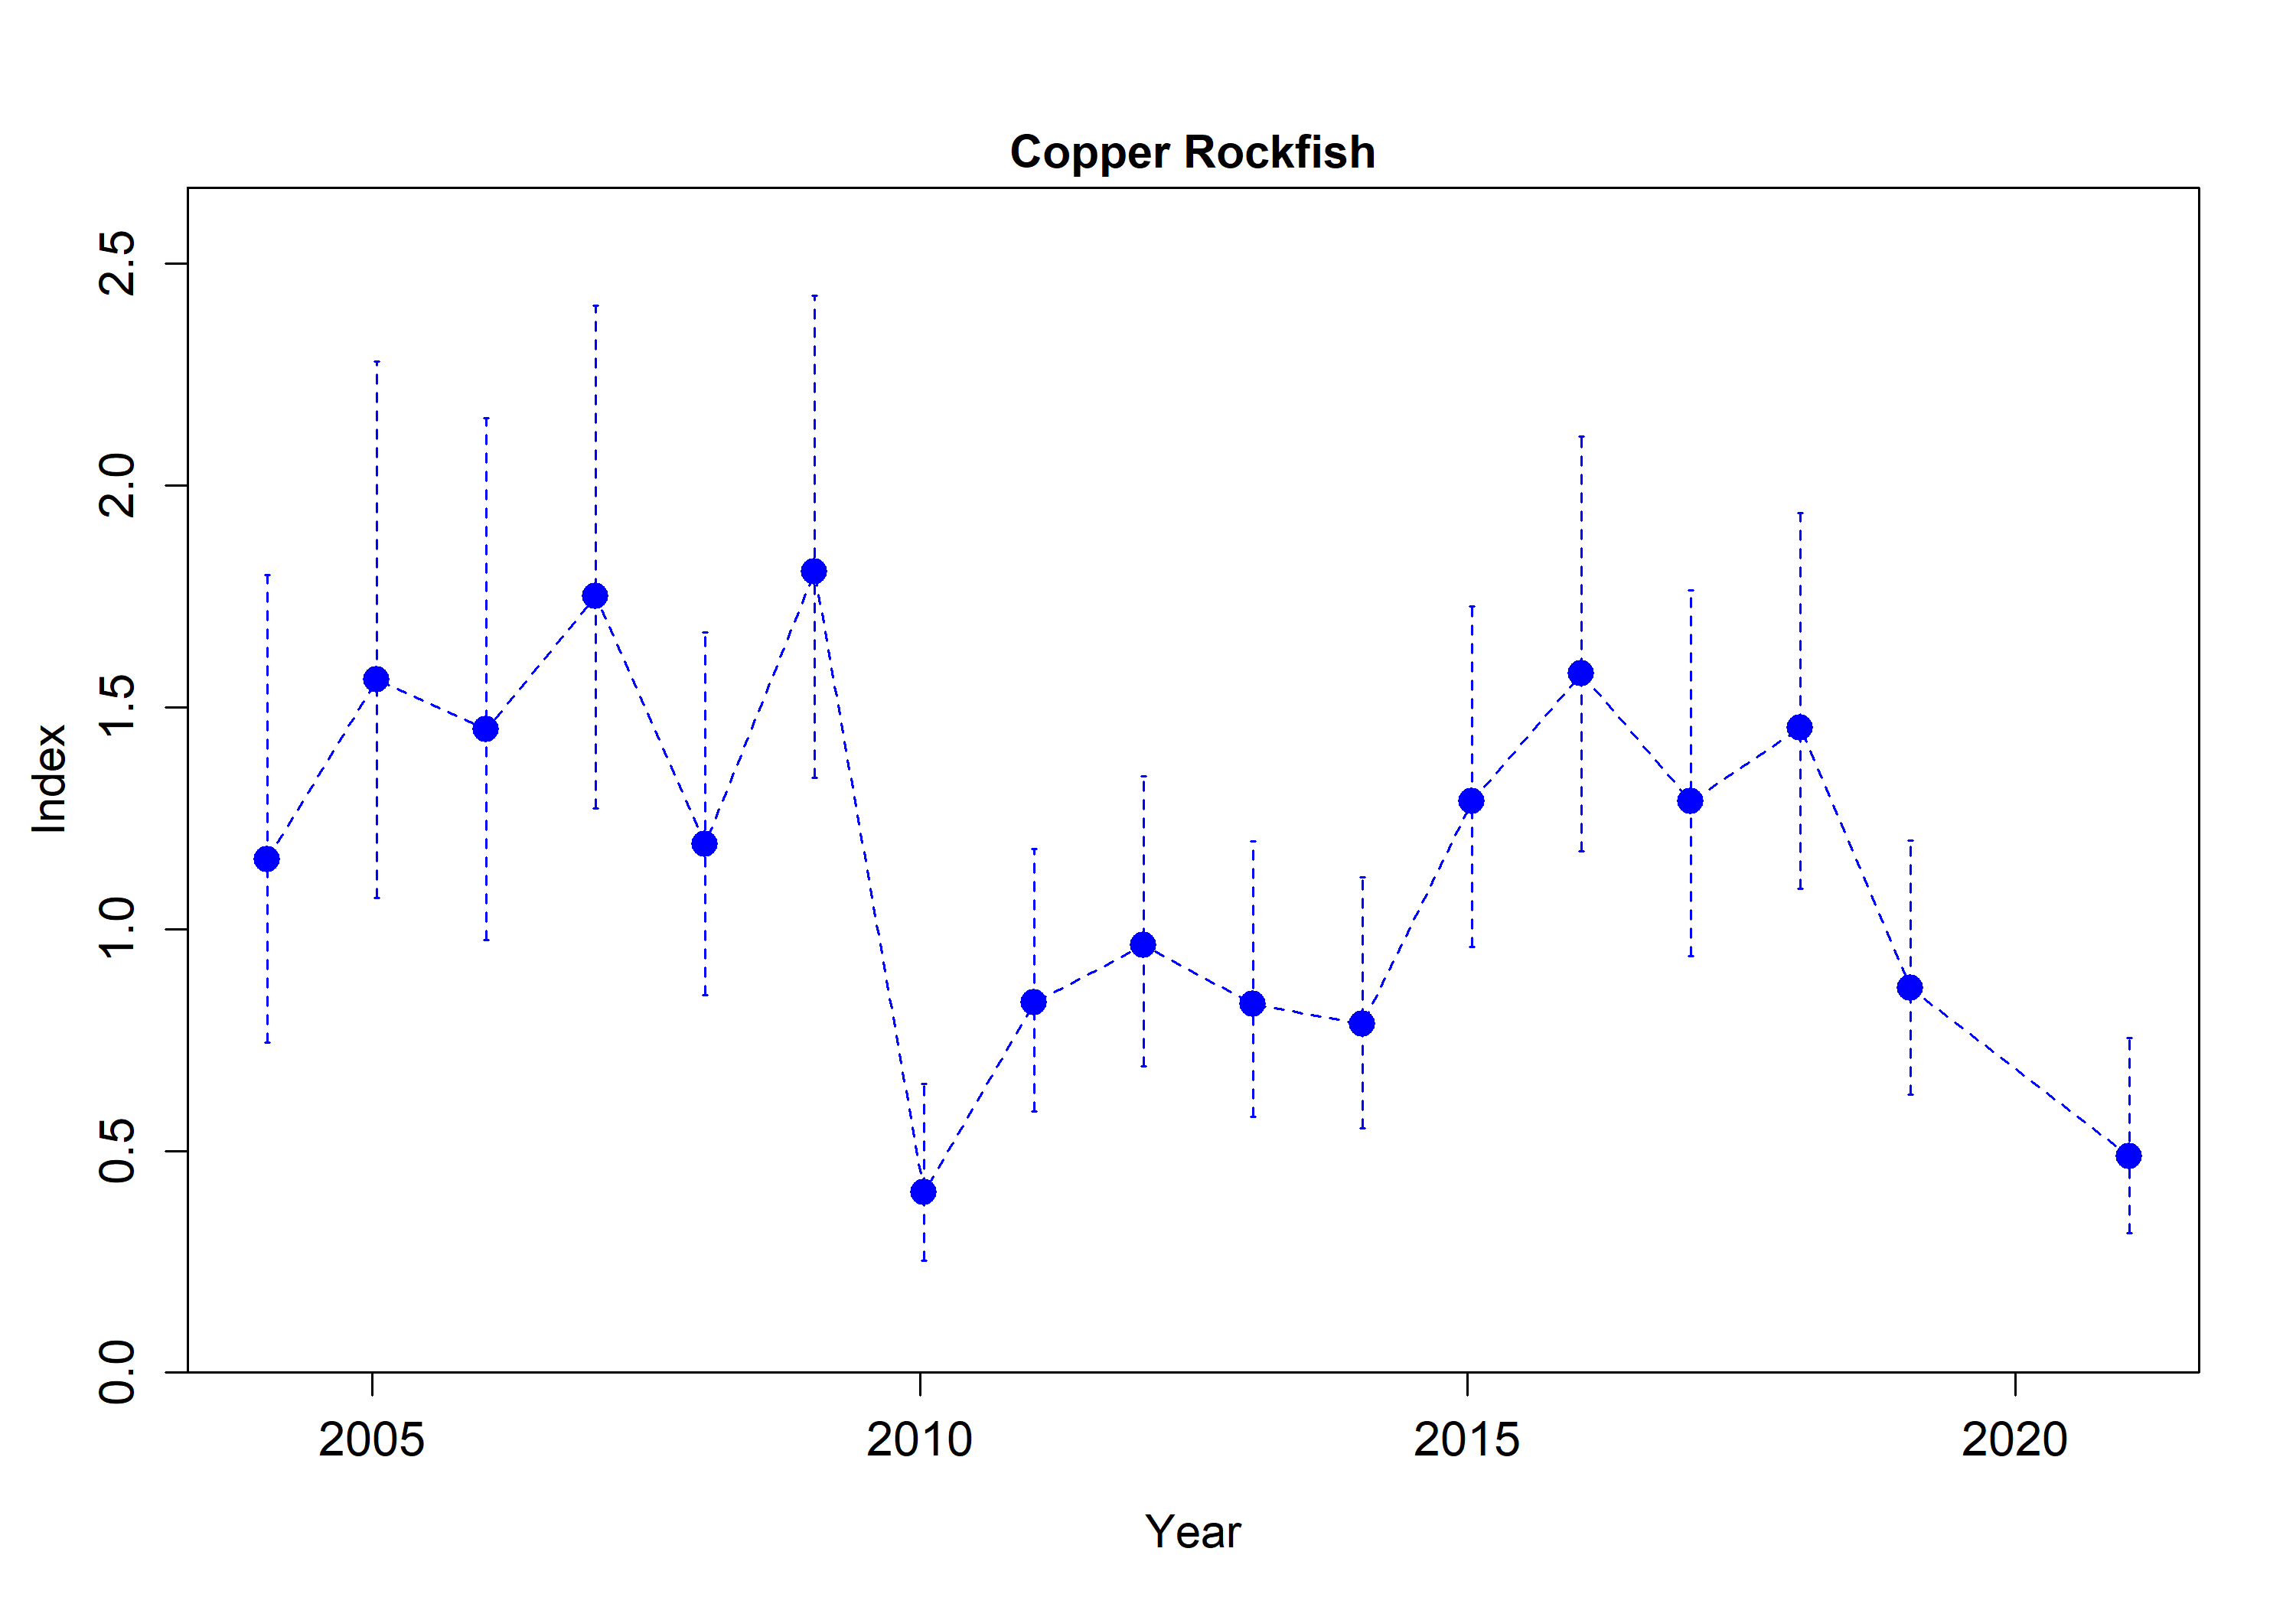
\includegraphics[width=1\textwidth,height=1\textheight]{C:/Assessments/2023/copper_rockfish_2023/docs/data_workshop/plots/nwfsc_hkl_glm_negbin_main_year_site_hook_drop_and_re_Index.png}
\caption{A preliminary relative index of abundance calculated using
available data between 2004-2021 estimated using a generalized linear
mixed model including fixed effects for year, site, hook, and drop and
angler random effects. Once data from 2022 are available estimation of
the index of abundance across additional model structures will be
explored (source: NWFSC Hook and Line survey).\label{fig:hkl-index}}
\end{figure}

\hypertarget{nwfsc-west-coast-groundfish-bottom-trawl-survey}{%
\subsubsection{NWFSC West Coast Groundfish Bottom Trawl
Survey}\label{nwfsc-west-coast-groundfish-bottom-trawl-survey}}

The NWFSC West Coast Groundfish Bottom Trawl (WCGBT) survey has been
conducted across the West Coast annually since 2003 (there was no
sampling conducted in 2020 due to the COVID-19 pandemic). The number of
observations of copper rockfish by the NWFSC WCGBT survey are limited
due to the sample gear (bottom trawl) which is deployed on soft bottom
substrate. A summary of the observations by this survey between
2003-2021 can be found
\href{https://www.pcouncil.org/documents/2022/05/f-3-attachment-4-detailed-summary-of-available-data-to-support-west-coast-groundfish-stock-assessments-in-2023-electronic-only.pdf\#page=111}{online}.
The majority of observations of copper rockfish by the NWFSC WCGBT
survey occur south of Point Conception. The limited number of tows by
year will likely prevent the calculation of an index of abundance for
this survey. Additionally, observations using bottom trawl gear may not
be informative of population trends for rocky-habitat and or hard-bottom
associated species such as copper rockfish. However, the collected
otolith and length data from this survey will be used to help inform
growth (north = 195 samples, south = 584 samples).

\hypertarget{additional-data-sources-being-considered}{%
\subsubsection{Additional Data Sources Being
Considered}\label{additional-data-sources-being-considered}}

Multiple inquiries regarding additional data that could be considered to
generate indices of abundance and/or composition data have been made for
the follow datasets:

\begin{itemize}
\tightlist
\item
  SMURF data
\item
  \href{https://www.piscoweb.org/}{PISCO}
\item
  \href{https://www.reefcheck.org/country/usa-california/}{ReefCheck}
\item
  CDFW ROV data
\end{itemize}

Finally, the southern California Publicly Owned Treatment Works (POTW)
dataset has been evaluated for observations of copper rockfish. However,
the number of copper rockfish observations were determined to be too
limited for the creation of a potential index of abundance.

\hypertarget{fishery-dependent}{%
\subsection{Fishery-Dependent}\label{fishery-dependent}}

Fishery-dependent indices will be explored for both the CPFV (PC) and
Private/Rental (PR) fleets using onboard observer data and dockside
sampling, i.e., angler interviews. The indices of abundance for each
fleet will likely only be developed through 2019 due to the reduction in
trips and sampling in 2020 due to the COVID-19 pandemic and regulation
changes in 2021. Additionally, the recreational fleet actively avoided
copper rockfish in 2023.

\hypertarget{composition-data}{%
\section{Composition Data}\label{composition-data}}

\hypertarget{commerical-length-compositions}{%
\subsection{Commerical length
compositions}\label{commerical-length-compositions}}

\begin{figure}
\centering
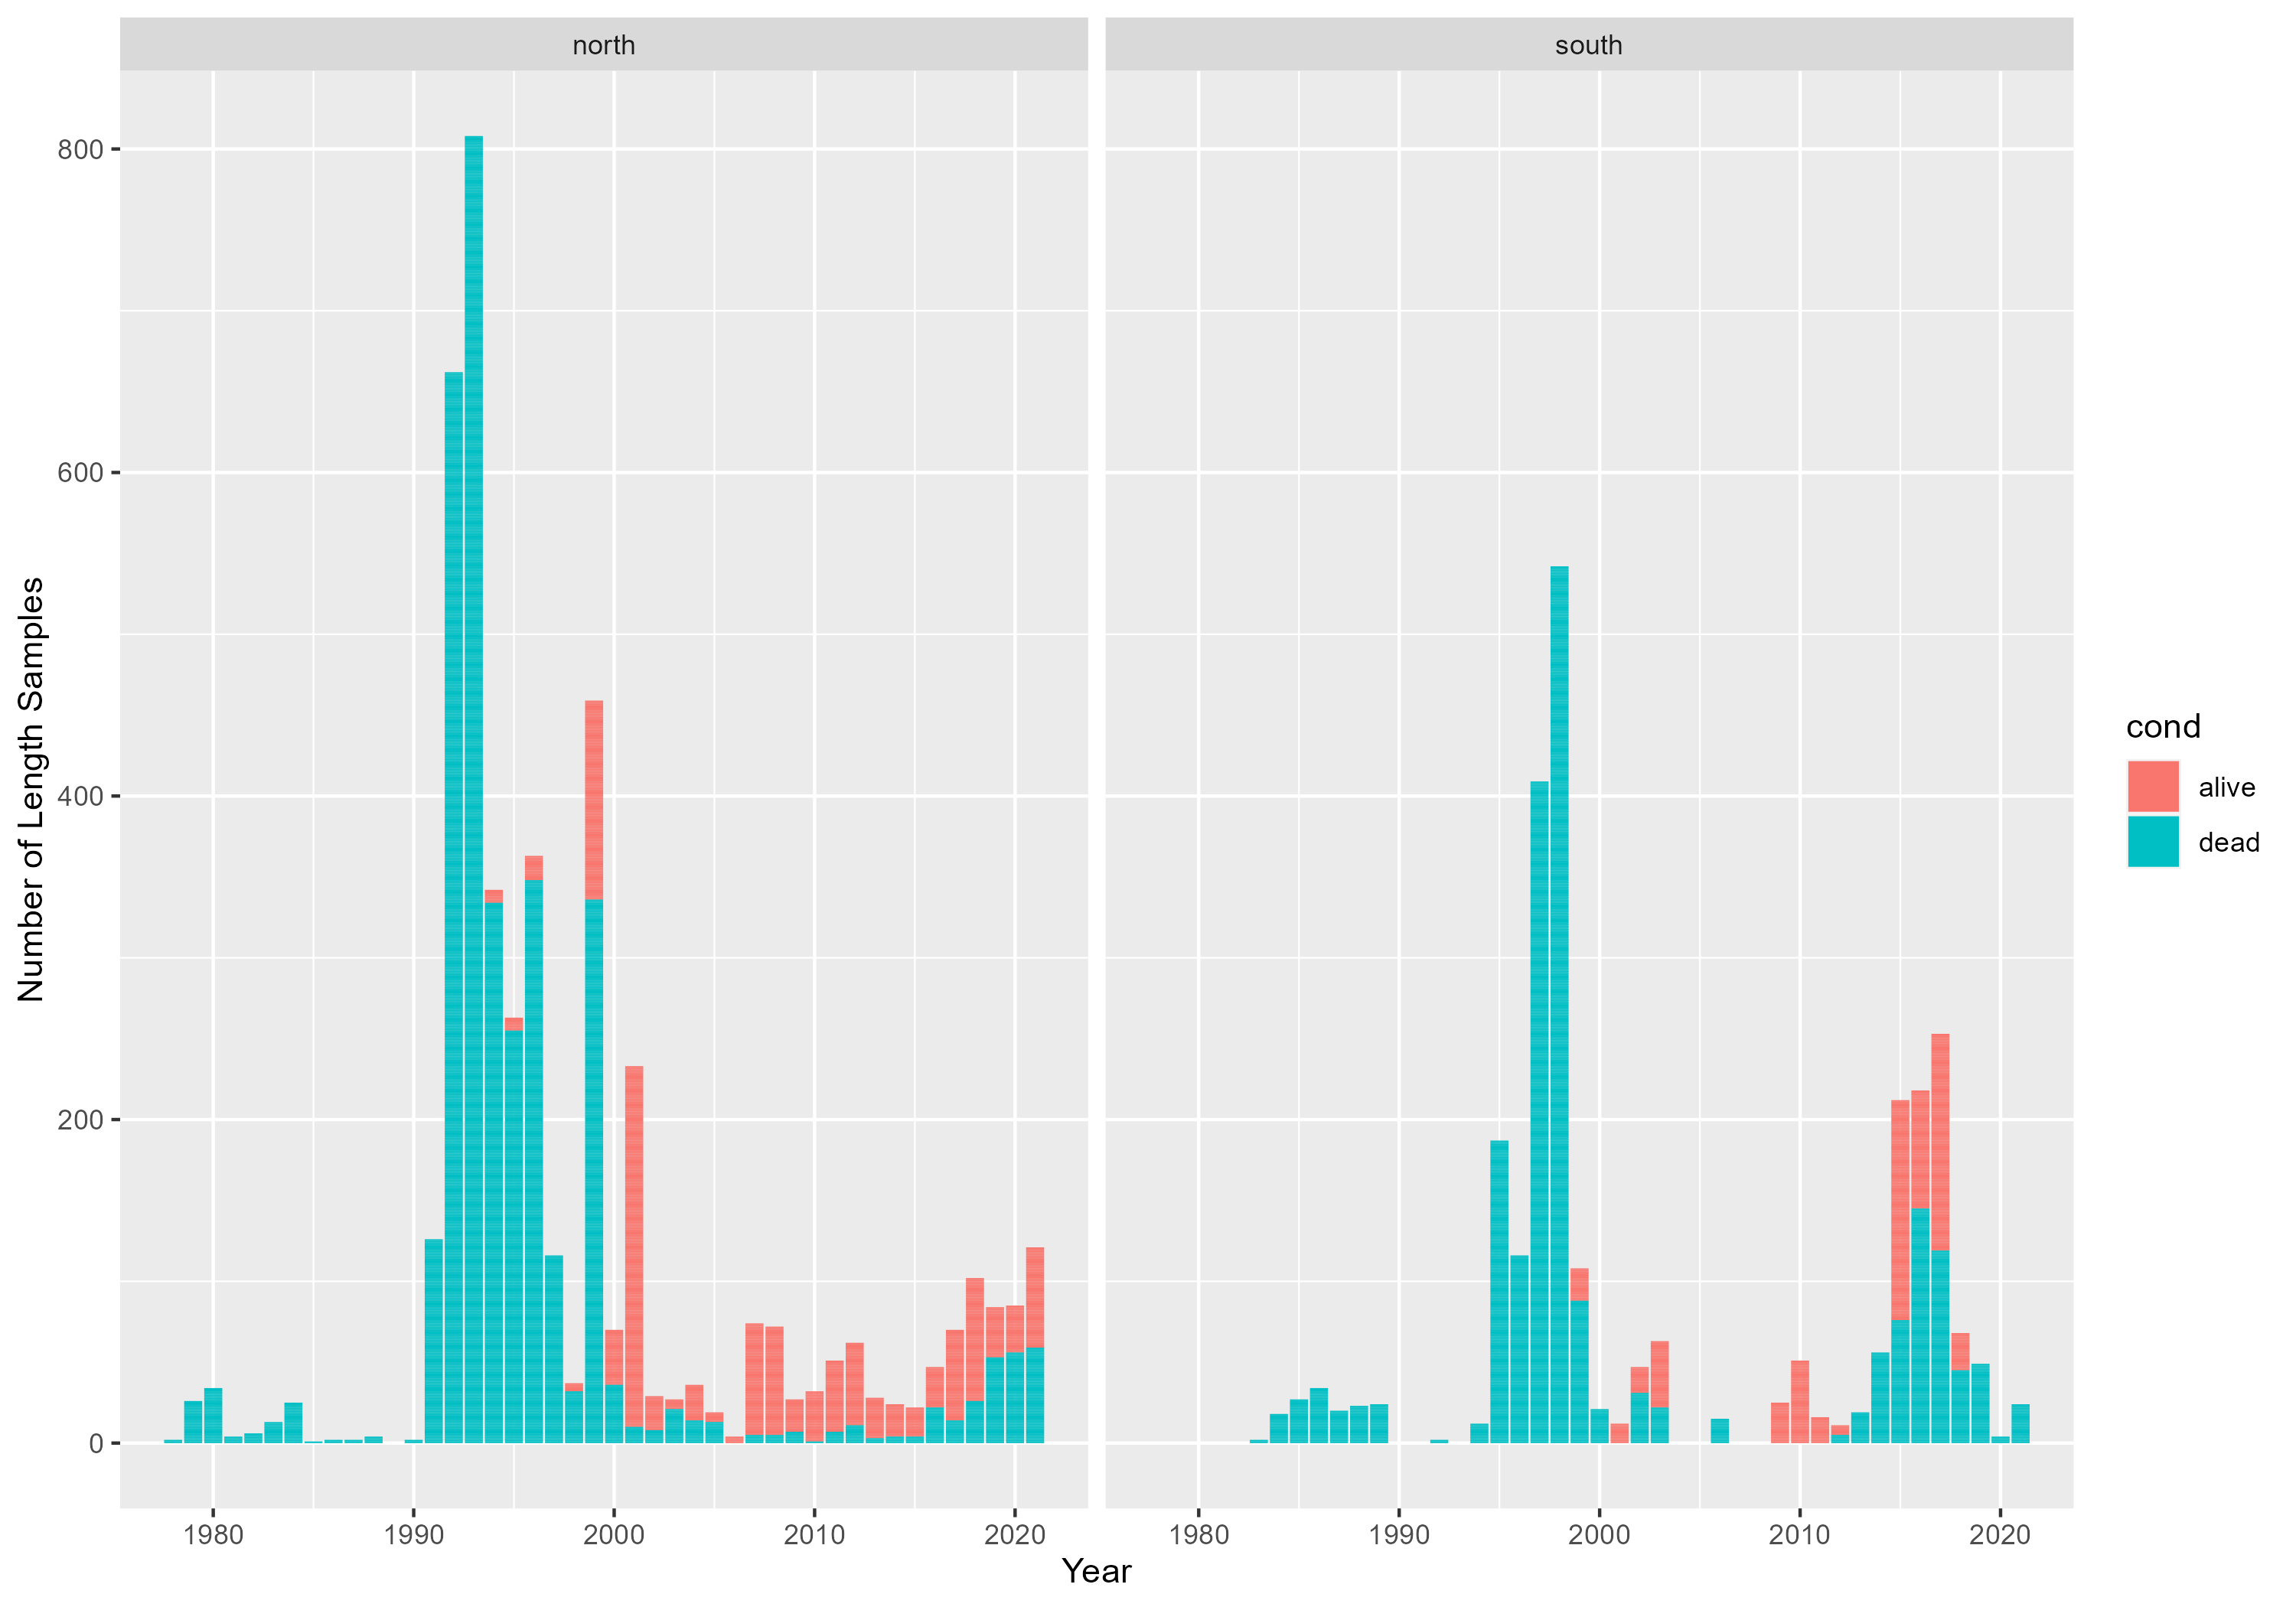
\includegraphics[width=1\textwidth,height=1\textheight]{C:/Assessments/2023/copper_rockfish_2023/docs/data_workshop/plots/com_length_samples_by_cond_area_year.png}
\caption{The number of length samples by year from live and dead copper
rockfish from the area south and north of Point Conception. Since 1981,
there are a total of 3,517 dead and 1,099 live length samples north of
Point Conception and 553 live and 2,135 dead length samples south of
Point Conception (source: PacFIN).\label{fig:com-length-n}}
\end{figure}

The majority of lengths are from hook and line gear for each area:

\begin{itemize}
\tightlist
\item
  North of Point Conception (total lengths = 4,616):

  \begin{itemize}
  \tightlist
  \item
    4,268 from hook and line gear,
  \item
    32 from net gear,
  \item
    139 from pot gear,
  \item
    15 from troll gear, and
  \item
    162 from trawl gear.
  \end{itemize}
\item
  South of Point Conception (total lengths = 2,688):

  \begin{itemize}
  \tightlist
  \item
    2,585 from hook and line gear,
  \item
    24 from net gear,
  \item
    39 from trawl gear, and
  \item
    36 from shrimp trawl gear.
  \end{itemize}
\end{itemize}

\begin{figure}
\centering
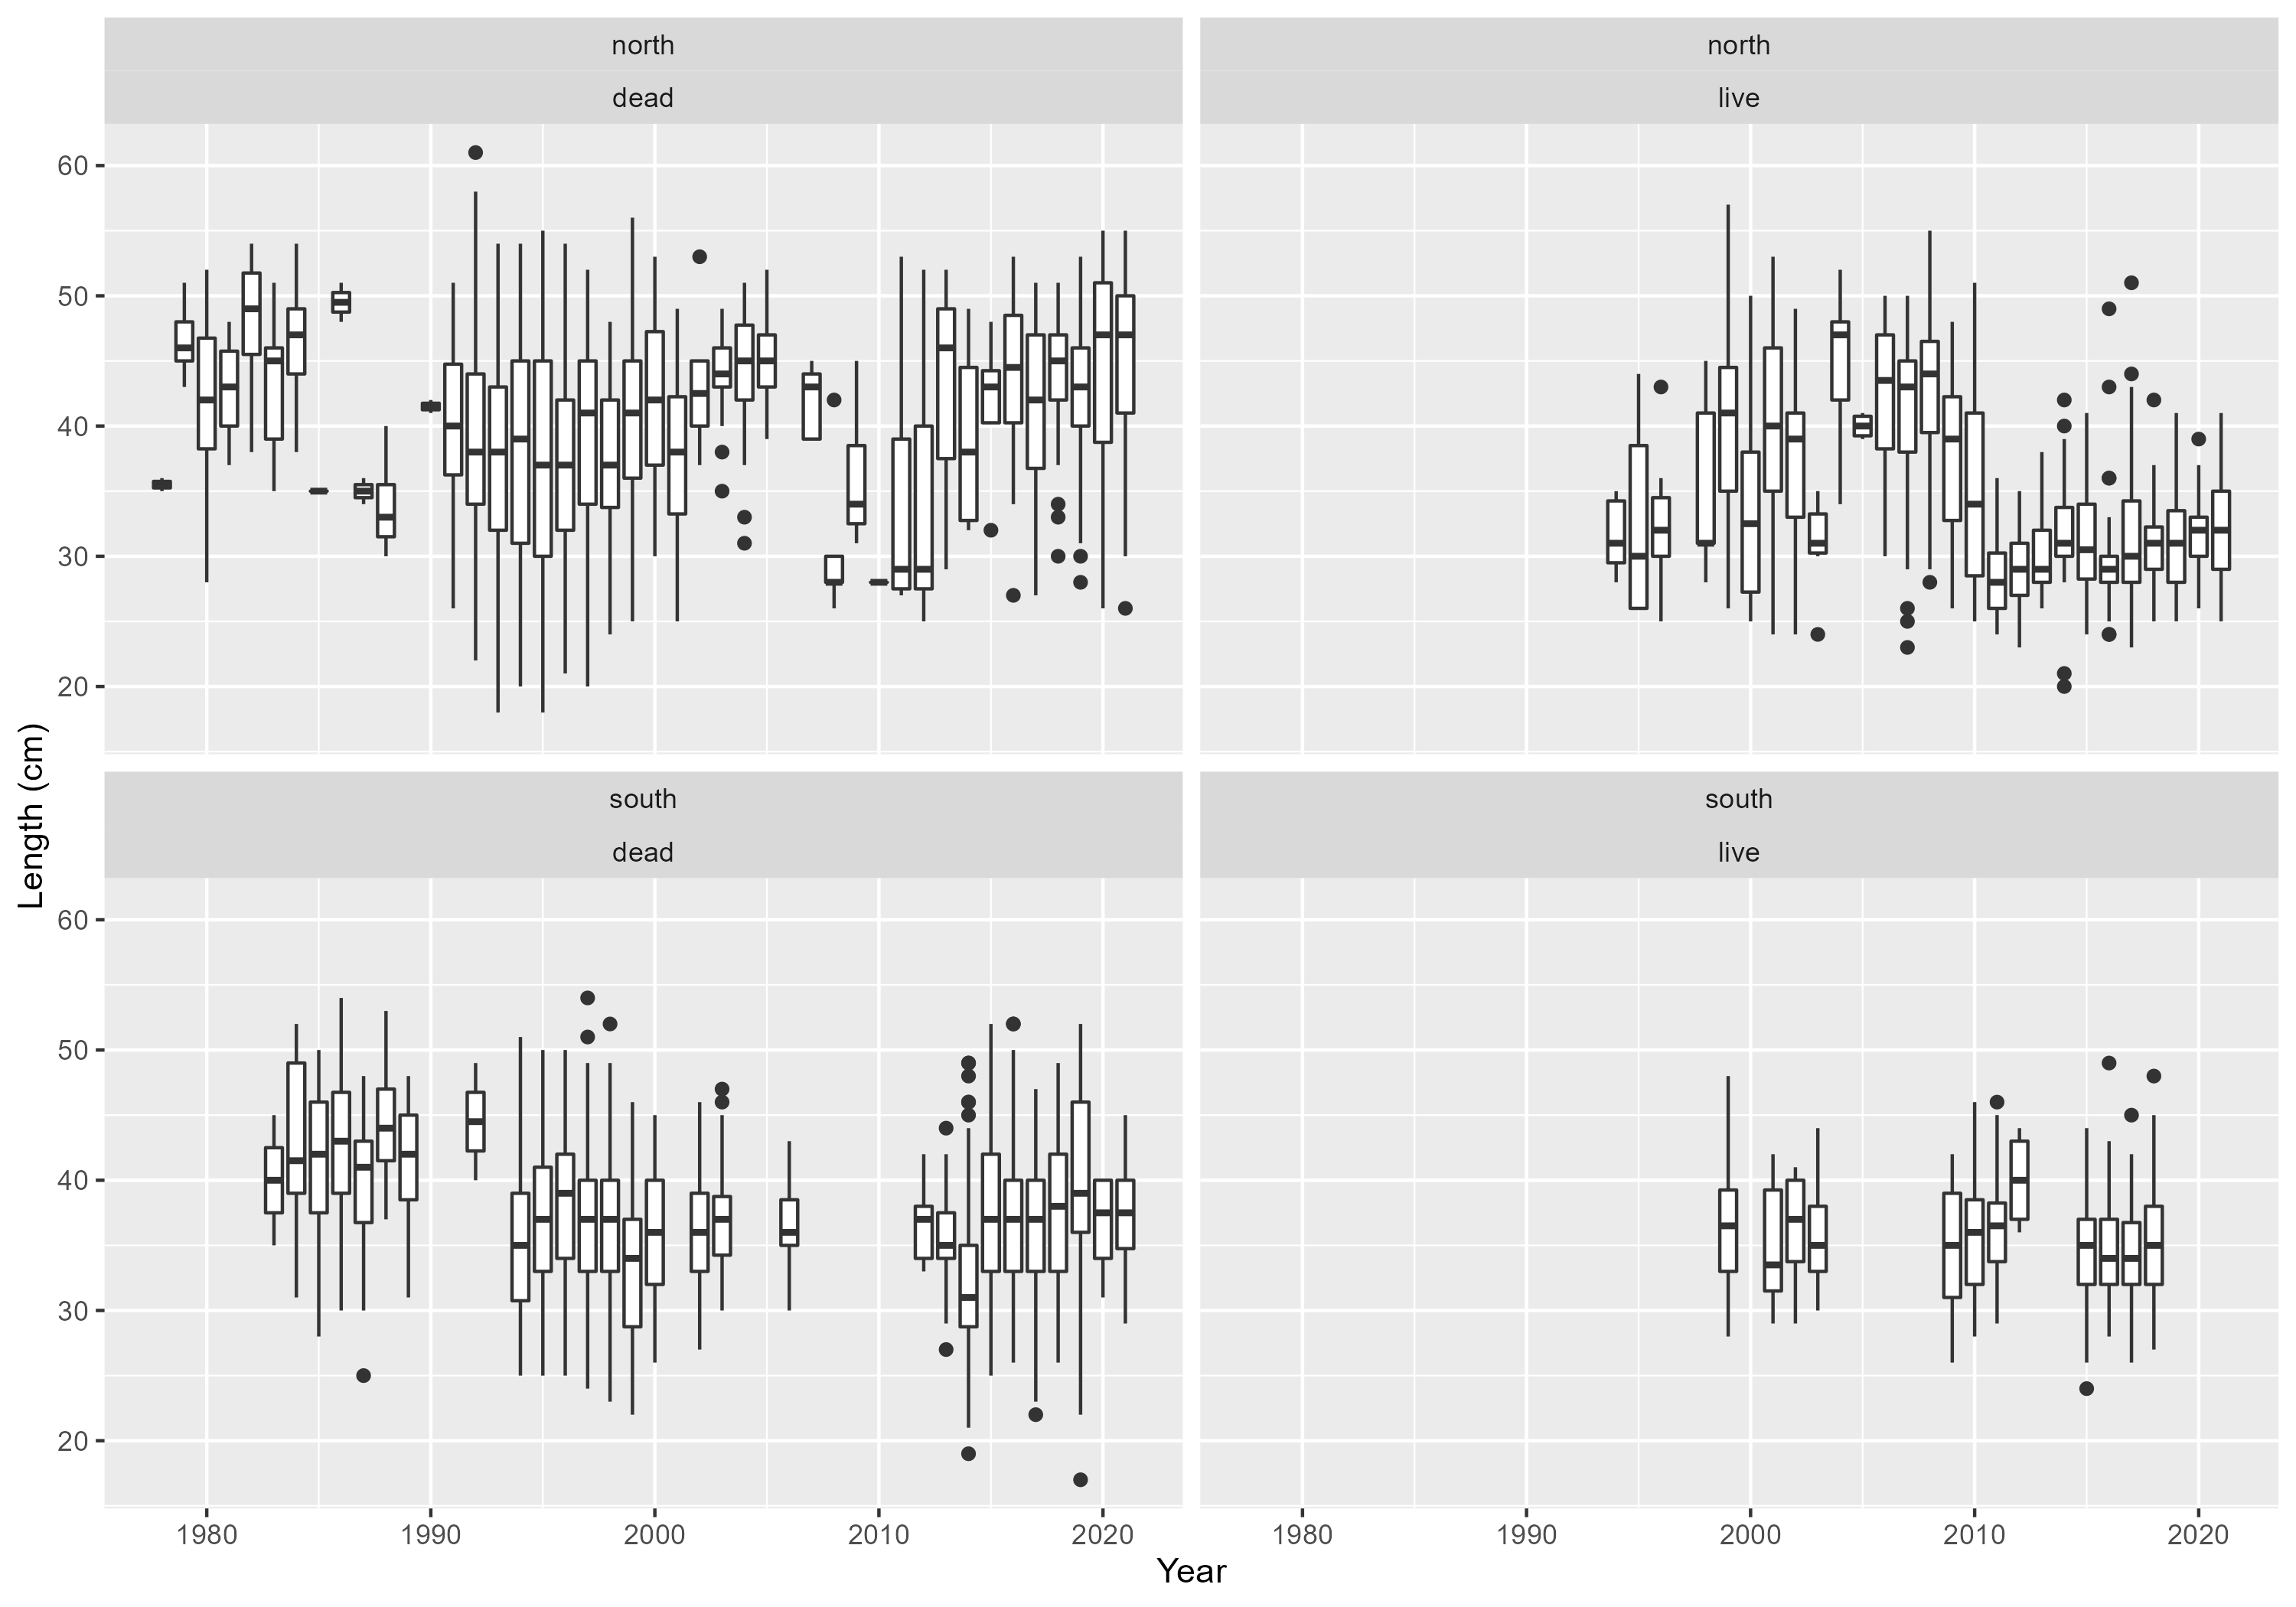
\includegraphics[width=1\textwidth,height=1\textheight]{C:/Assessments/2023/copper_rockfish_2023/docs/data_workshop/plots/length_boxplot_by_cond_area_year.png}
\caption{The distribution of length samples by year from live and dead
copper rockfish from the area south and north of Point Conception. The
black horizontal line within each box indicates the median length
observed that year where the median is defined as an equal number of
observations from that year that are greater than and lesser than that
value. The lower range of each box indicates the 25th percentile where
25 percent of observations that year are less than that length. The
upper range of each box indicates the 75th percentile where 75 percent
of observations that year are less than that length (source:
PacFIN).\label{fig:com-length-dist}}
\end{figure}

\begin{figure}
\centering
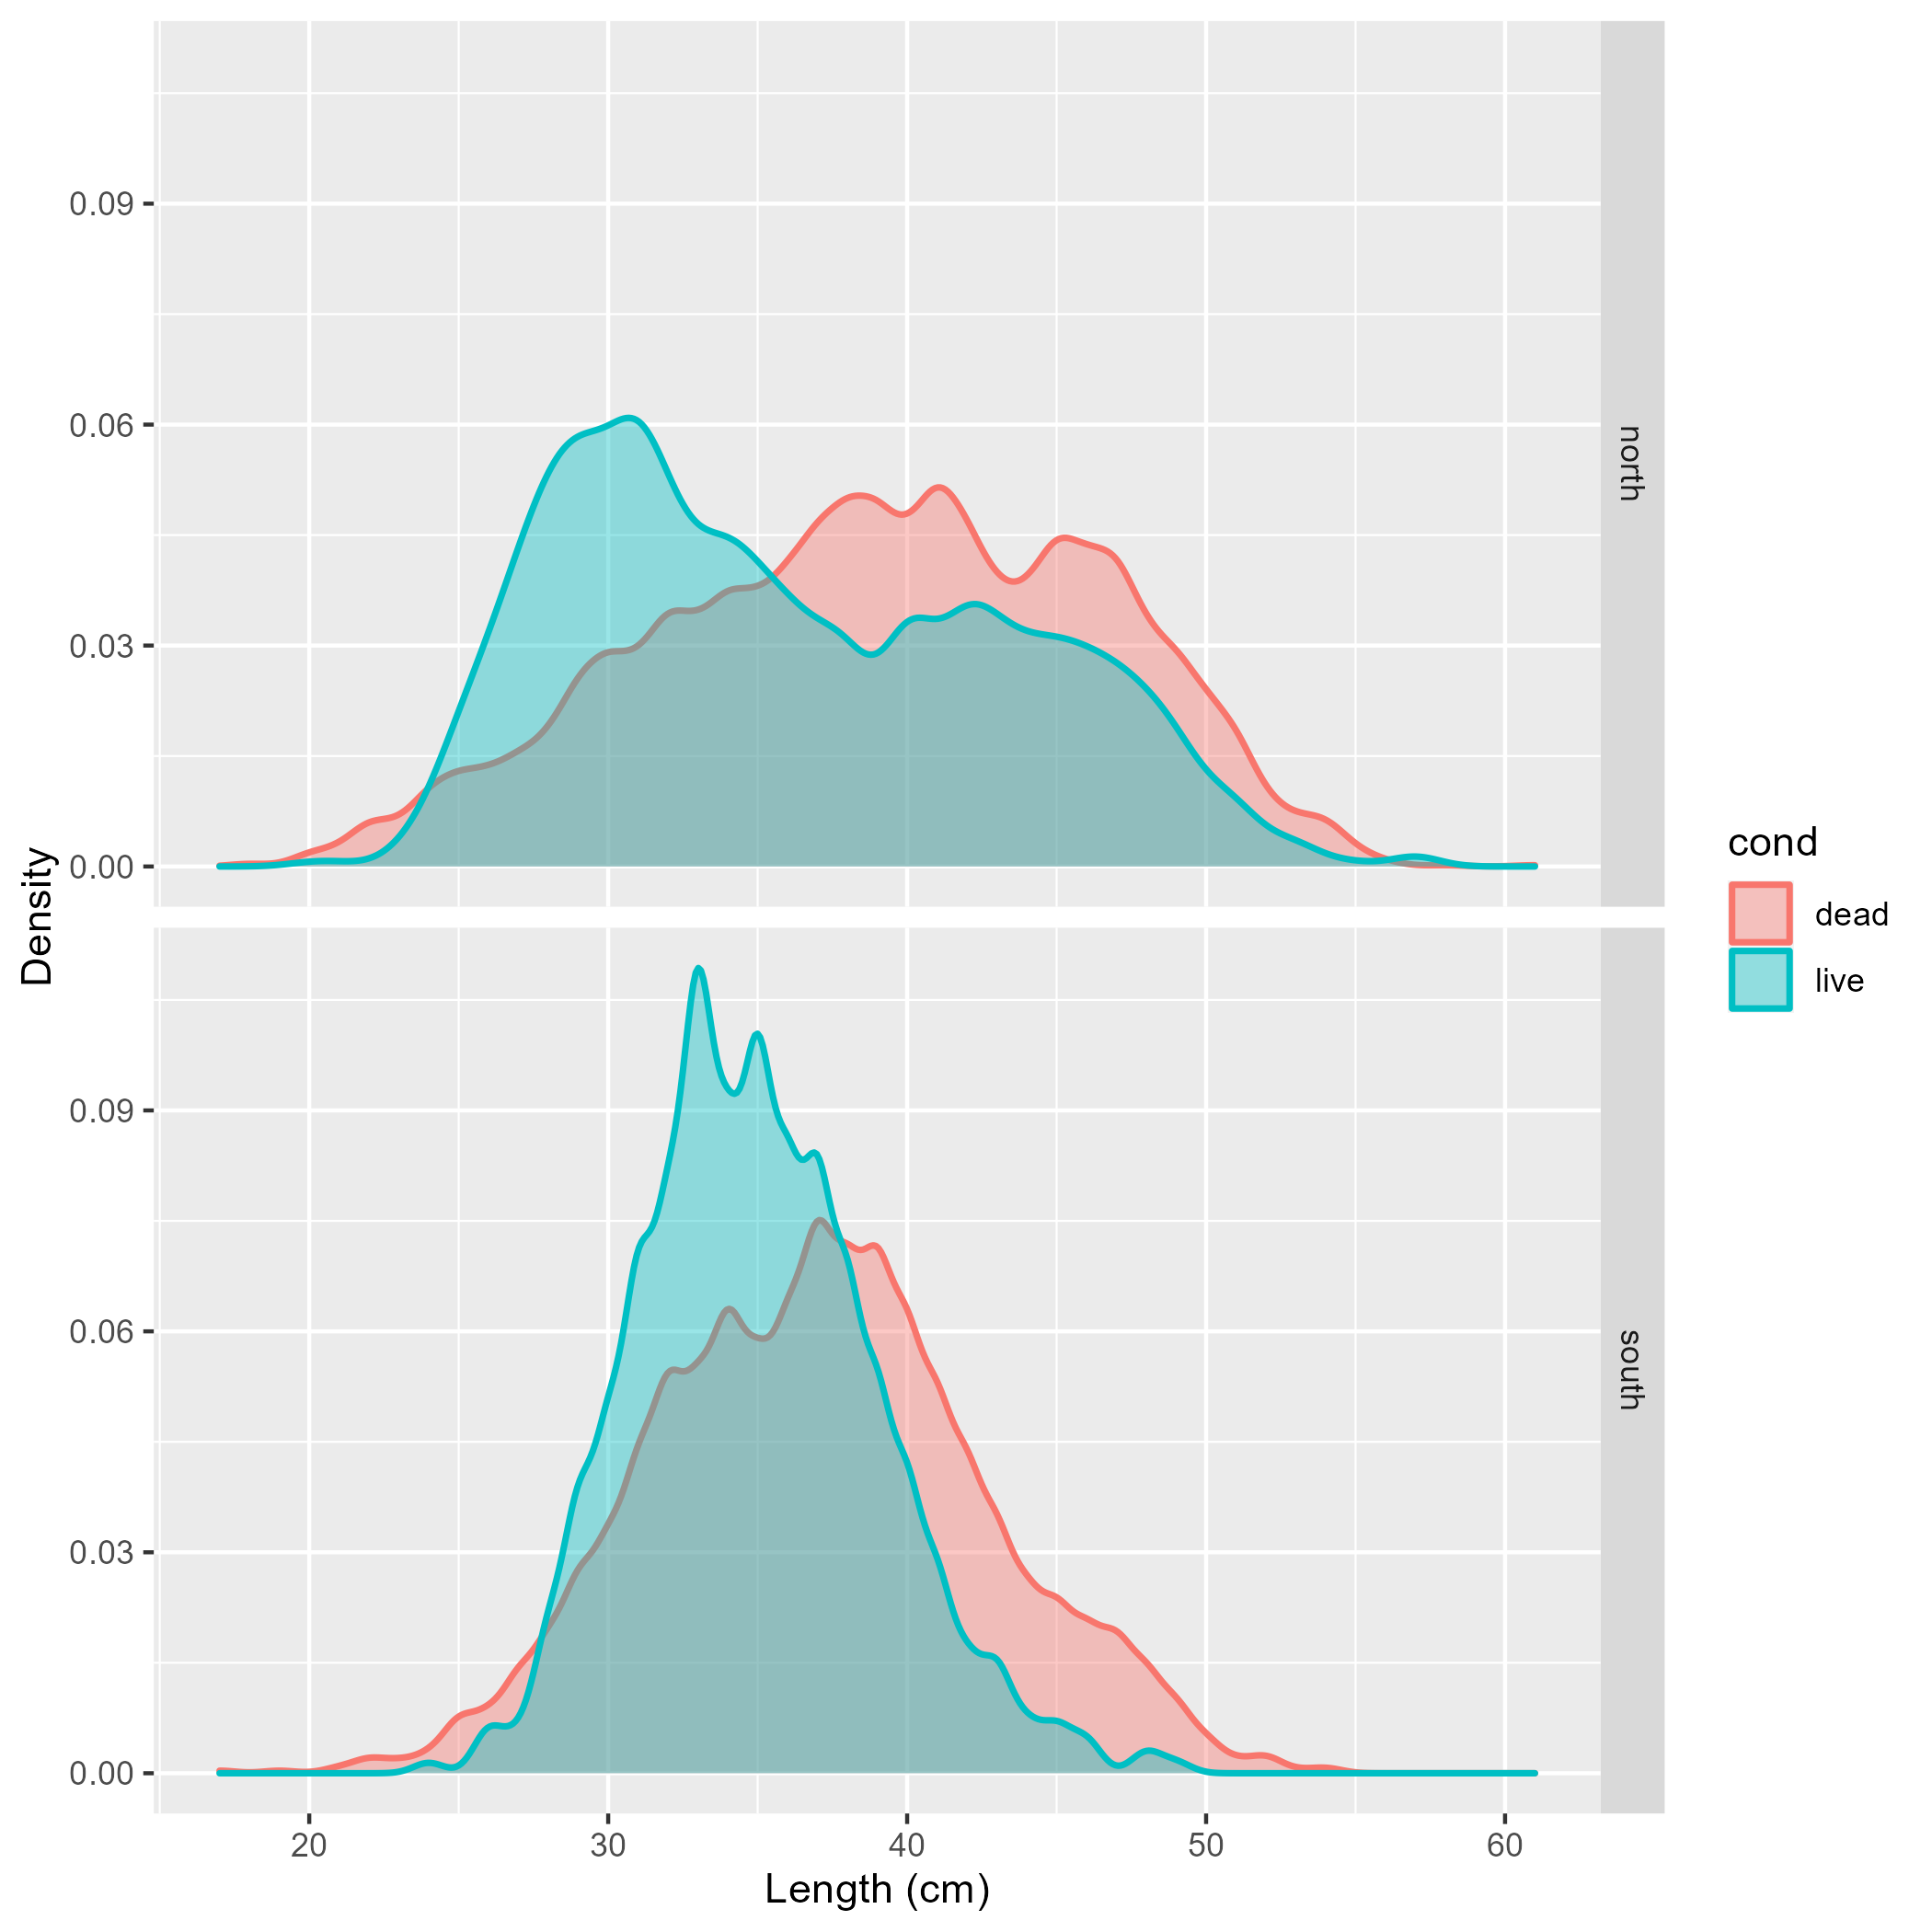
\includegraphics[width=1\textwidth,height=1\textheight]{C:/Assessments/2023/copper_rockfish_2023/docs/data_workshop/plots/length_denstity_by_cond_area.png}
\caption{The density of size selected by landed condition, live or dead,
for each area across all years (source:
PacFIN).\label{fig:com-marginal-length-dist}}
\end{figure}

\begin{figure}
\centering
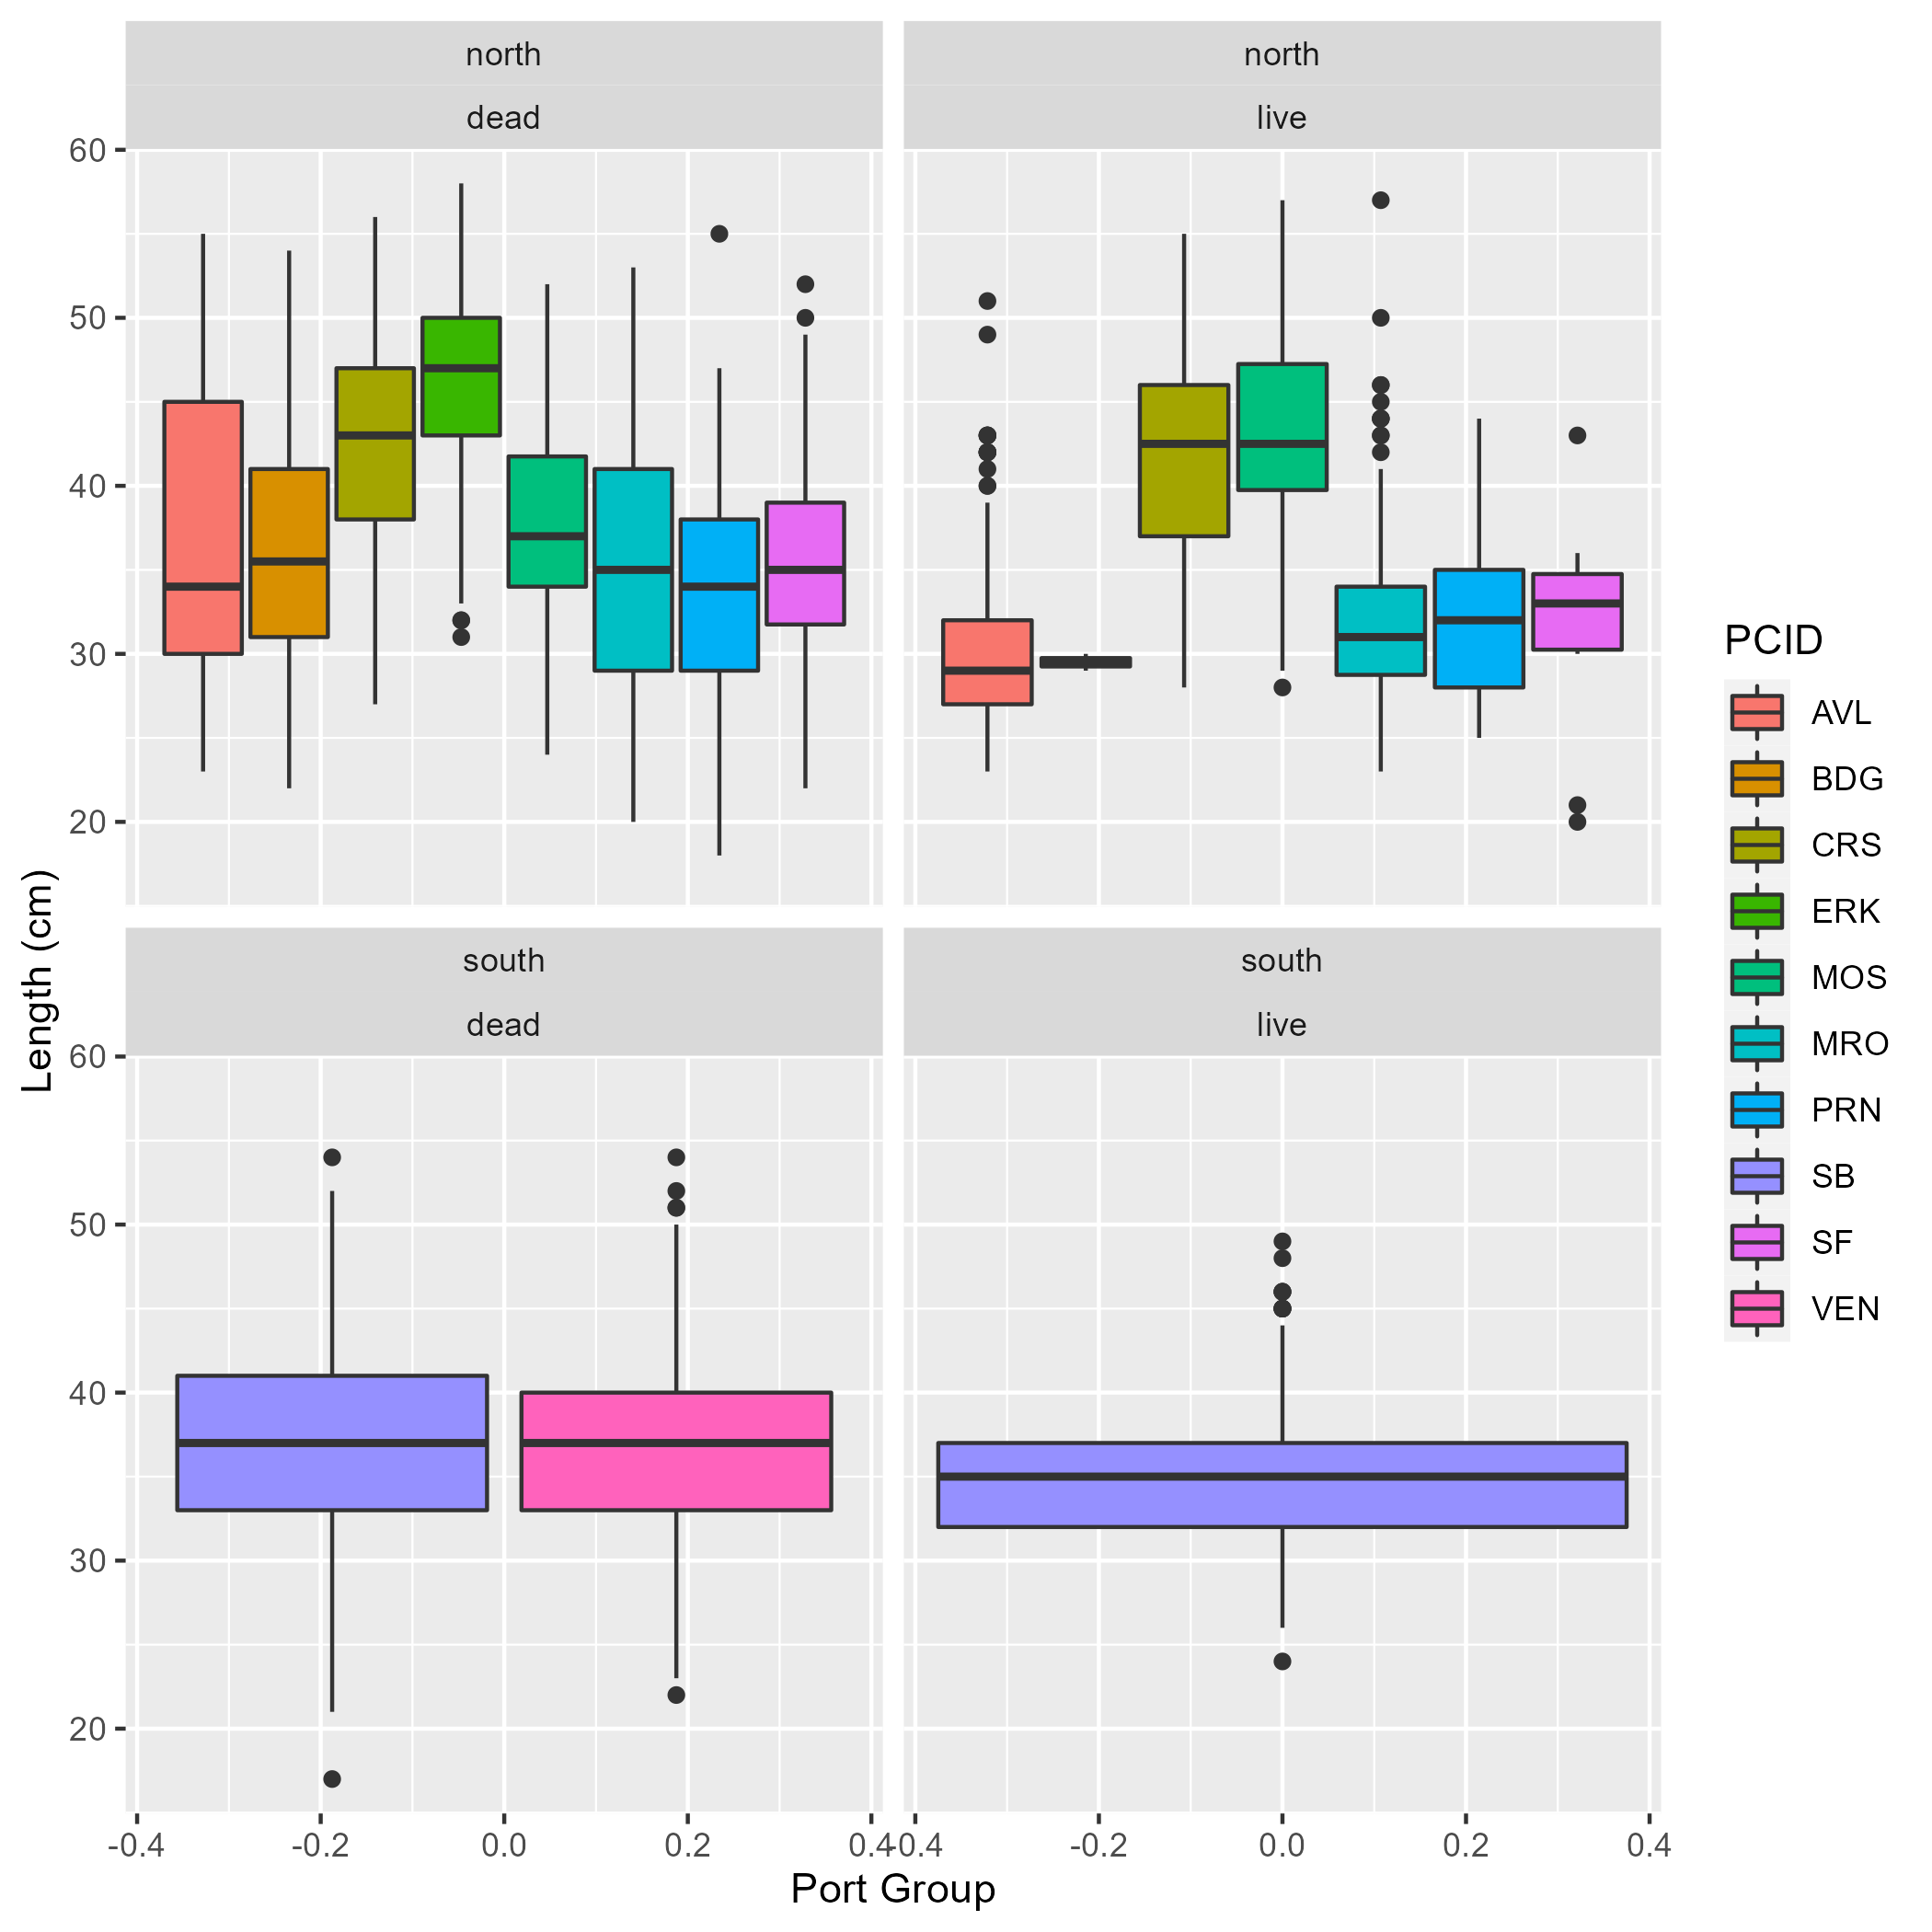
\includegraphics[width=1\textwidth,height=1\textheight]{C:/Assessments/2023/copper_rockfish_2023/docs/data_workshop/plots/boxplot_length_by_port_area_cond_filtered_by_100n.png}
\caption{Boxplot of lengths by landed port, area, and fish condition
(live or dead) across all years. Only ports with greater than 100 length
samples (live + dead \textgreater{} 100 samples) across all years are
shown. The Ventura (VEN) and Santa Barbara (SB) ports are south of Point
Conception. The ports north of Point Conception are Avila (AVL), Morro
Bay (MRO), Moss Landing (MOS), Half Moon Bay (PRN), San Francisco (SF),
Bodega Bay (BDG), Eureka (ERK), Crescent City (CRS) (source:
PacFIN).\label{fig:com-boxplot-length-port}}
\end{figure}

\hypertarget{recreational-length-compositions}{%
\subsection{Recreational length
compositions}\label{recreational-length-compositions}}

The recreational length composition data summarized below represent data
pulled from RecFIN collected by either the MRFSS (1980 - 2003) or CRFS
(2004 - 2022) sampling programs. There are additional data sources that
contain historical length samples from the CPFV fleets (1975-1979 from
Collins and Crooke, 1987-1998 from Deb Wilson-Vandenberg, and 1986-1989
from Alley and Ono) that will be evaluated and used within each
assessment model as appropriate but are not included here.

The total number of length samples within RecFIN across MRFSS and CRFS
are:

\begin{itemize}
\tightlist
\item
  North of Point Conception (total lengths = 38,994):

  \begin{itemize}
  \tightlist
  \item
    11,969 from CPFV, and
  \item
    27,025 from Private/Rental vessels.
  \end{itemize}
\item
  South of Point Conception (total lengths = 31,036):

  \begin{itemize}
  \tightlist
  \item
    23,535 from CPFV, and
  \item
    7,501 from Private/Rental vessels.
  \end{itemize}
\end{itemize}

In RecFIN there are lengths from shoreside modes that were not included
in the analysis presented below (north of Point Conception = 148 and
south = 20). All lengths below represent retained fish. There were
limited length observations of released fish (north = 52 and south =
187).

\begin{figure}
\centering
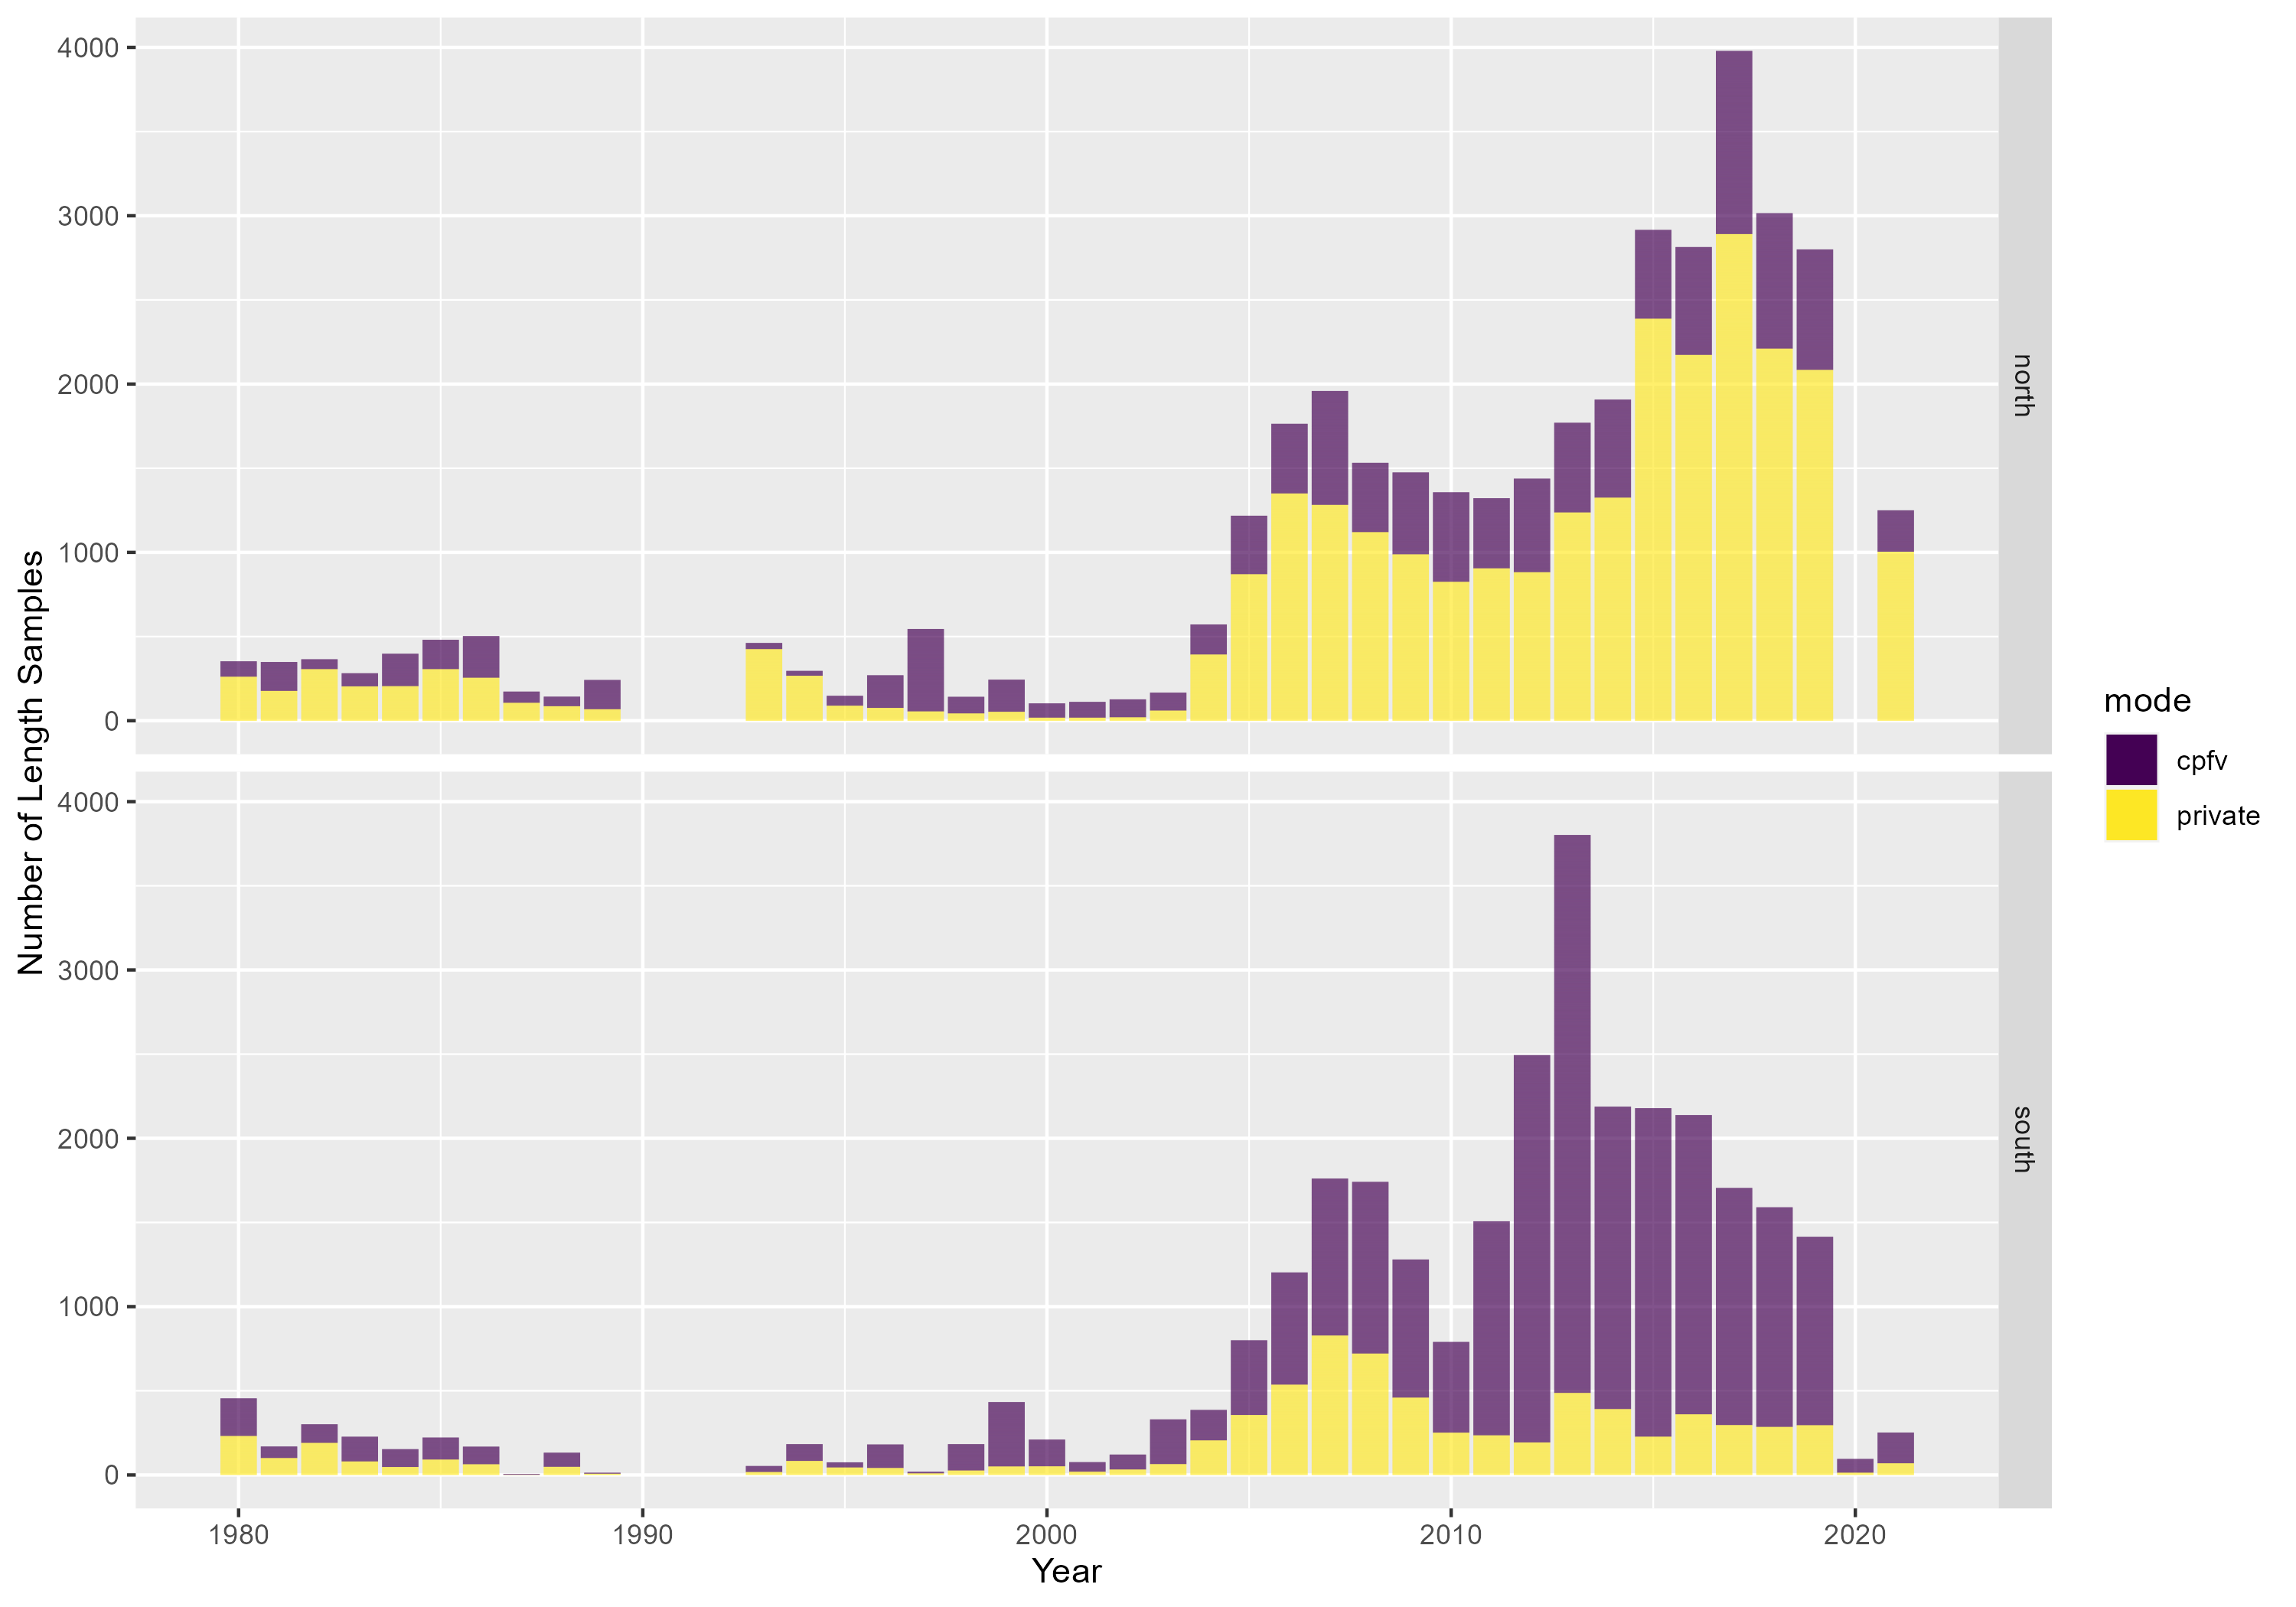
\includegraphics[width=1\textwidth,height=1\textheight]{C:/Assessments/2023/copper_rockfish_2023/docs/data_workshop/plots/rec_length_samples_by_area_year.png}
\caption{The number of length samples by year and mode for copper
rockfish for areas south and north of Point Conception. Since 1980,
there are a total of 11,969 CPFV and 27,025 Private/Rental length
samples north of Point Conception and 23,535 CPFV and 7,501
Private/Rental length samples south of Point Conception (source:
RecFIN).\label{fig:rec-length-samples}}
\end{figure}

\begin{figure}
\centering
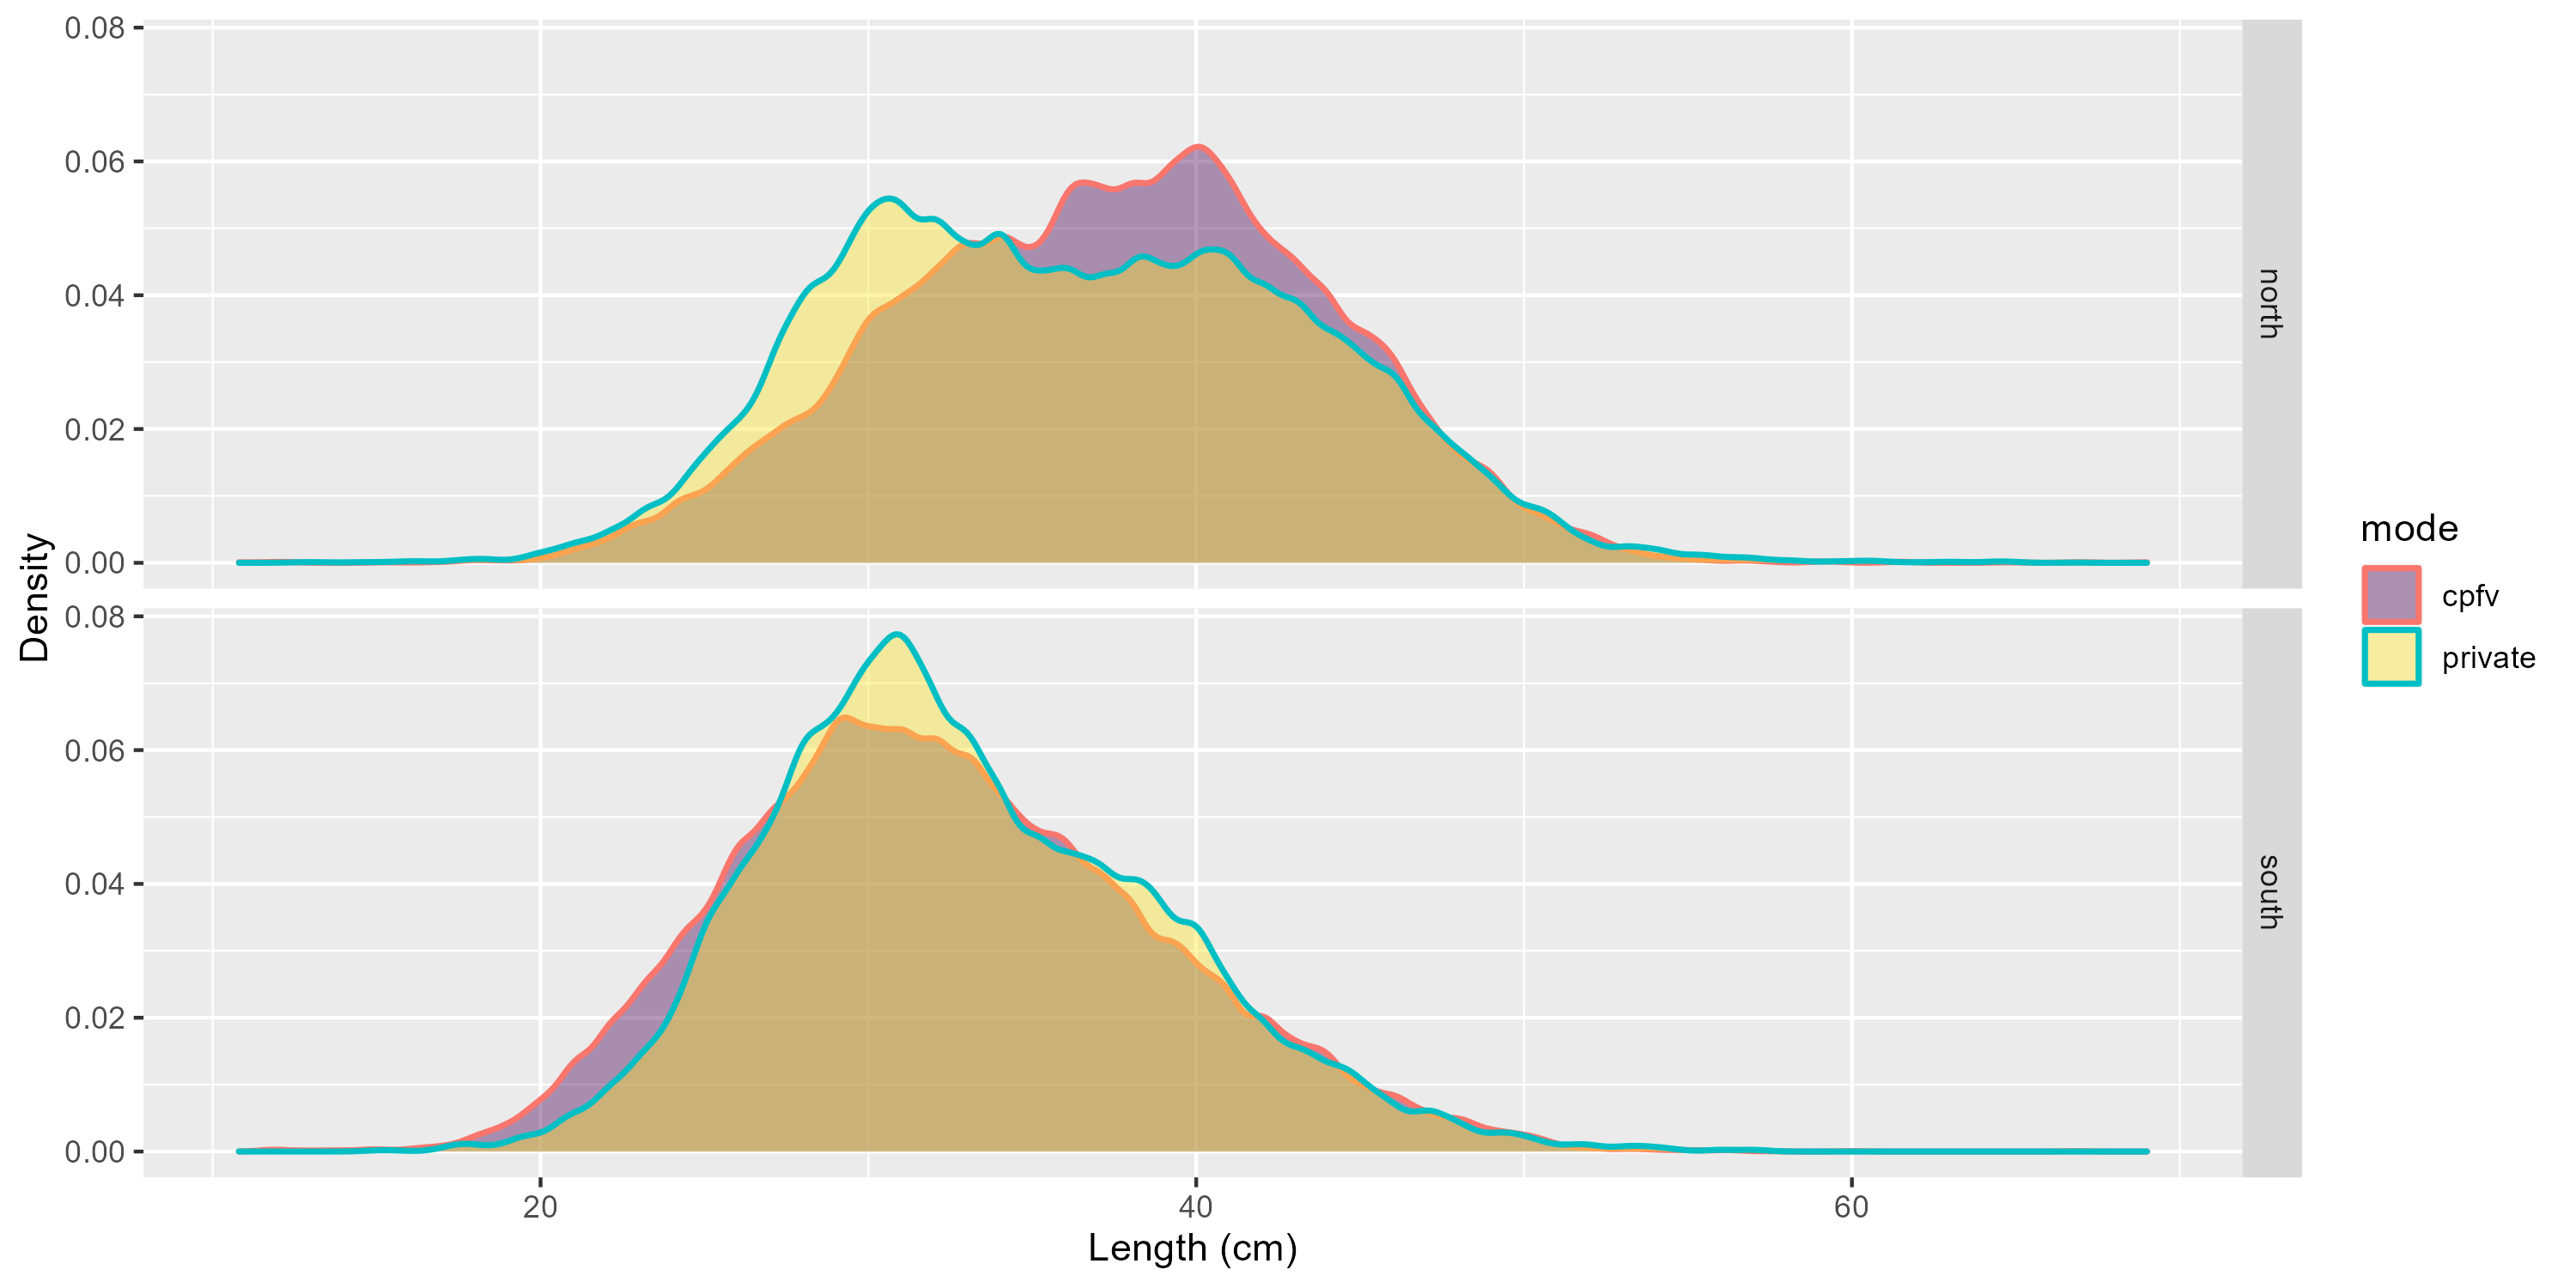
\includegraphics[width=1\textwidth,height=1\textheight]{C:/Assessments/2023/copper_rockfish_2023/docs/data_workshop/plots/all_length_dist_by_mode_area.png}
\caption{The density of size selected by mode, CPFV or Private/Rental,
for each area across all years (source:
RecFIN).\label{fig:rec-length-dist}}
\end{figure}

\hypertarget{potential-bias-in-length-sampling-with-cpfv-trip-duration}{%
\subsubsection{Potential bias in length sampling with CPFV trip
duration}\label{potential-bias-in-length-sampling-with-cpfv-trip-duration}}

The CDFW California Recreational Fisheries Survey (CRFS) collects length
samples from fish caught on CPFVs. These samples are collected by both
staff on board CPFV trips and at the docks when vessels return. On board
CRFS staff are unable to sample overnight trips with as high a frequency
as day trips. In many cases, these overnight trips may reach
destinations that are farther from port and therefore experience lower
fishing rates and contain larger fish.This could result in a bias in
length distributions aggregated across trip duration if sites with
larger fish are under-sampled.

The STAT examined the length distributions of fish sampled on trips of
varying duration by district.Overnight trips only occur in the southern
California sampling districts 1 (San Diego, Orange, and Los Angeles
counties) and 2 (Ventura and Santa Barbara counties).Some separation in
copper rockfish length frequencies is observed in district 1.

\begin{figure}
\centering
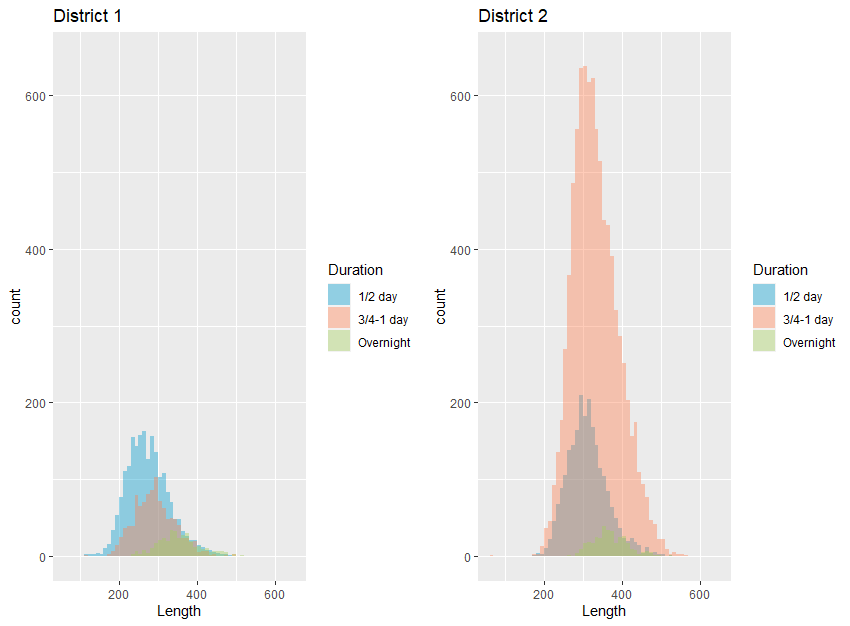
\includegraphics[width=1\textwidth,height=1\textheight]{C:/Assessments/2023/copper_rockfish_2023/docs/data_workshop/plots/CopperDurationDist12.png}
\caption{Copper rockfish length grequency by CPFV trip duration for CRFS
districts 1 \& 2 for 1/2 day, 3/4 day, and overnight fishing trips
(source: CRFS PC Onboard + Dockside
Surveys).\label{fig:cpfv-length-duration}}
\end{figure}

To determine if overnight trips are under-sampled, relative to their
frequency, we need to compare catch rates relative to sampling rates. A
sharp increase in the number of rockfish caught on overnight CPFV trips,
as well as other fish species, was observed in 2014 with catches
remaining relatively high through 2020. No increase was observed in the
single day trips. This was coincident with an increase in the number of
overnight trips being made in 2014. The increase in catch was likely
driven by the arrival of warm water which drove increases in pelagic
species. A large proportion of the trips made in 2014 listed tuna as the
target species. Many trips targeting pelagic species will also visit
sites to target groundfish, and this is the likely cause for the
coincident increase in groundfish catch.

\begin{figure}
\centering
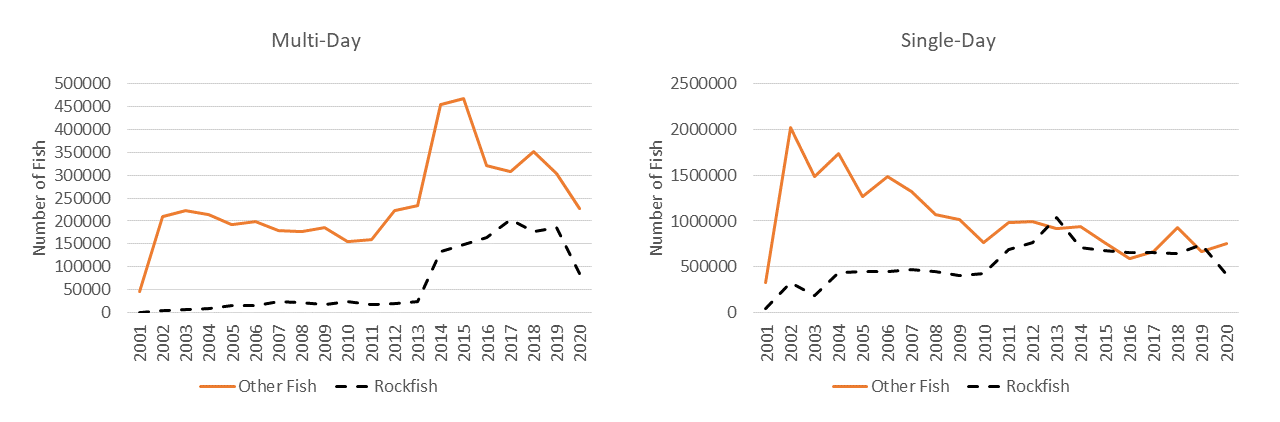
\includegraphics[width=1\textwidth,height=1\textheight]{C:/Assessments/2023/copper_rockfish_2023/docs/data_workshop/plots/cpfv_catch_multi_single.png}
\caption{CPFV catch of rockfish and non-rockfish on multi- and
single-day trips (source: CPFV
Logbooks).\label{fig:cpfv-catch-duration}}
\end{figure}

\begin{figure}
\centering
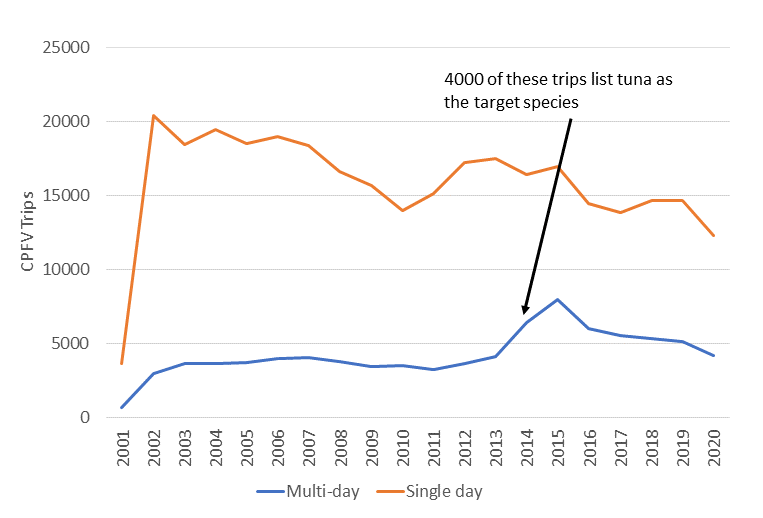
\includegraphics[width=1\textwidth,height=1\textheight]{C:/Assessments/2023/copper_rockfish_2023/docs/data_workshop/plots/cpfv_trips_multi_single.png}
\caption{The number of of multi- and single-day CPFV trips (source: CPFV
Logbooks).\label{fig:cpfv-trips-duration}}
\end{figure}

We calculated the percent of copper rockfish in southern California
caught on overnight trips relative to the total number of CPFV trips. We
compared this to the percent of copper rockfish length samples collected
from CPFVs that were taken from overnight trips. The lower proportion of
sampling relative to catch shows that there is under-sampling of these
trips. Given this, we will consider weighting length samples from CPFVs
according to trip duration to correct for this bias, particularly since
2014.

\begin{figure}
\centering
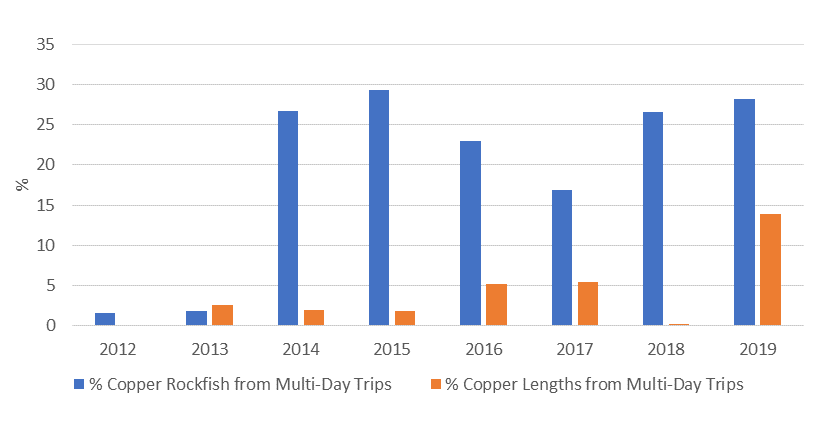
\includegraphics[width=1\textwidth,height=1\textheight]{C:/Assessments/2023/copper_rockfish_2023/docs/data_workshop/plots/cpfv_sampling_multi.png}
\caption{Percentage of copper rockfish caught on multi-day the
percentage of legth samples from mult-day trips (source: CPFV Logbooks
and CRFS PC Onboard and Dockside Surveys).\label{fig:cpfv-sampling}}
\end{figure}

Additionally, in order to understand the potential impact of biased and
unbiased sampling of trips by duration a simulation analysis was
conducted. The simulation analysis examined the average size of fish and
the variability around that average (standard deviation) by trip type:

\begin{itemize}
\tightlist
\item
  Single-day trip: average fish length of 31.9 cm with standard
  deviation of 6.1 cm, and
\item
  Multi-day trip: average fish length of 35.2 cm with standard deviation
  of 5.6 cm.
\end{itemize}

A bias (over-sampling of single-day trips) and an unbiased (sampling
aligns with the proportion of trip type) of a 1,000 total length sample
were randomly generated based on the average length and standard
deviation of observations from each trip type. The bias sampling
approach was based on the observed proportion of samples coming from
single-day trips. The most extreme difference in sampling proportion
observed in the data was used to generate the biased sample where 980
lengths were collected from single-day trips and 20 lengths were
collected from multi-day trips. The unbiased sample was based on the
proportion of single-day and multi-day trips observed between 2014 -
2018 where 81\% of the trips were single-day were 810 samples were from
single-day trips and 190 samples from multi-day trips were randomly
generated.

\begin{figure}
\centering
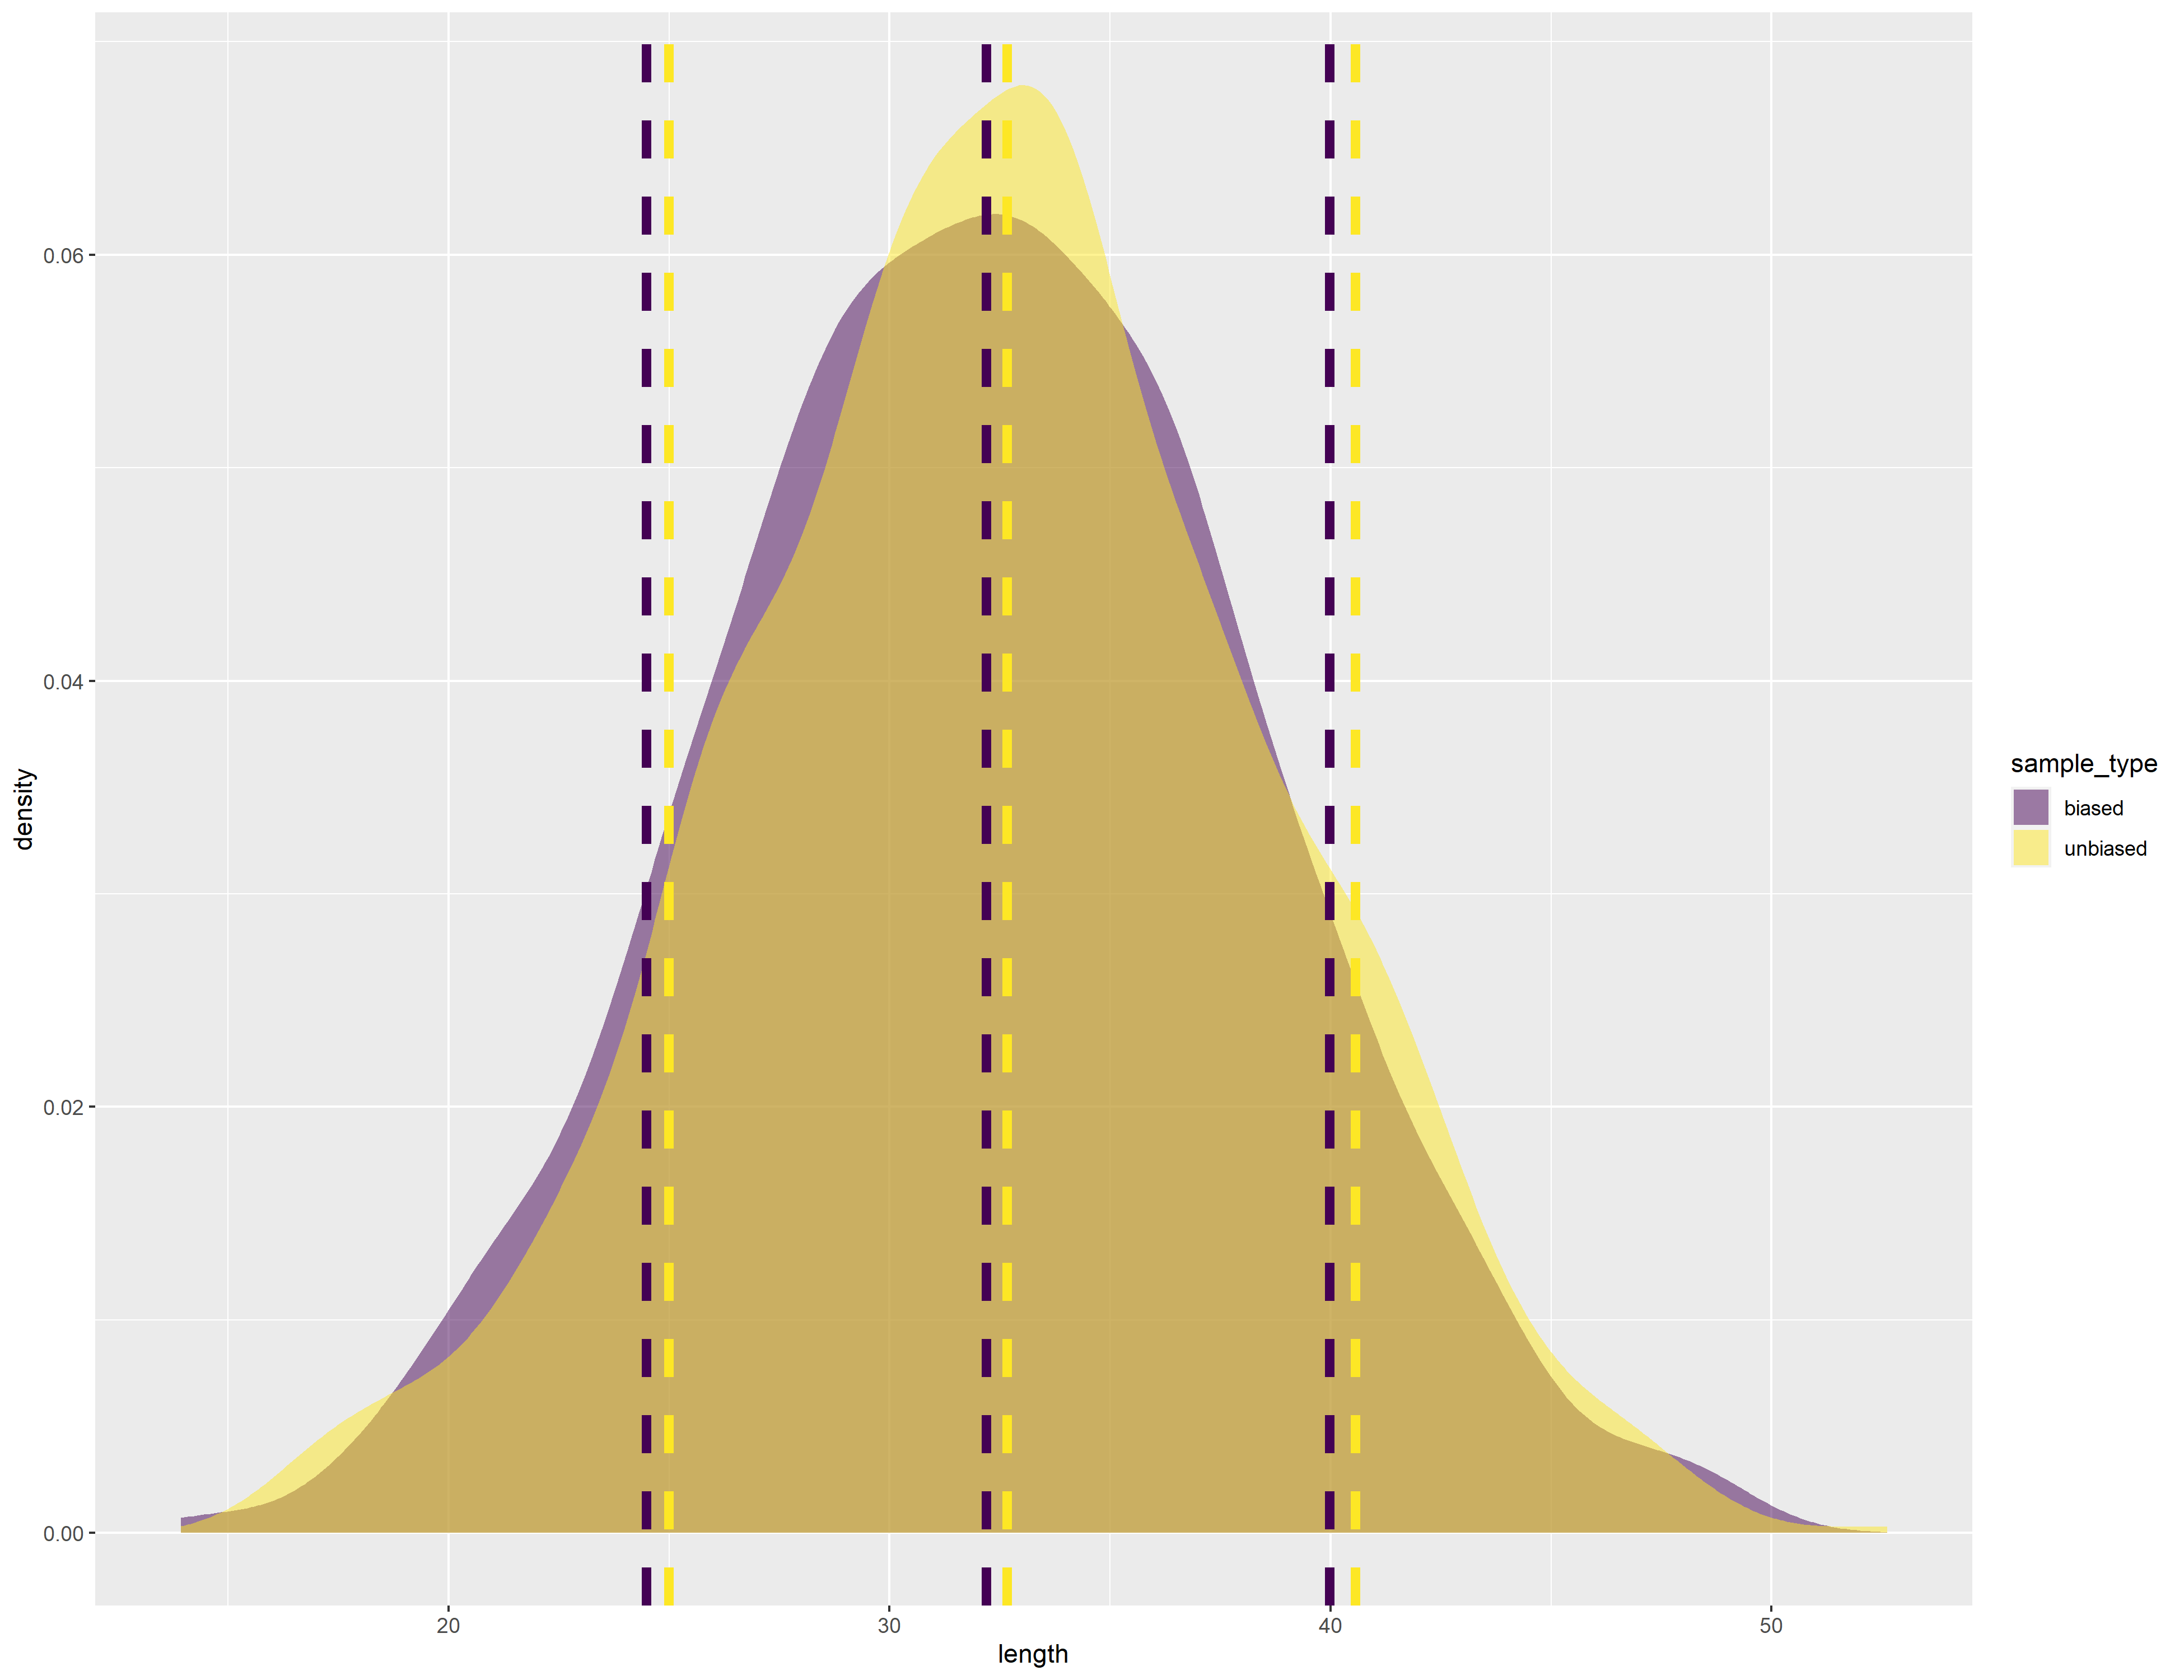
\includegraphics[width=1\textwidth,height=0.6\textheight]{C:/Assessments/2023/copper_rockfish_2023/docs/data_workshop/plots/cpfv_trip_sampling_bias_unbiased.png}
\caption{Simulated length distribution based on biased and unbiased
sampling of trip by duration (single-day or multi-day). The 10\%, 50\%,
and 90\% quartile from each sample type is show by the dashed verticle
lines. The median length (50\% quartile) of the unbiased sample was
approximately 0.5 cm greater than the median length from the biased
sample. While there are small differences in the length distribution
between the biased and unbiased samples, the difference is not great
enough to have a measurable impact the length composition data when
binned using 2 cm bins for use in an assessment model (source: simulated
samples based on CPFV Logbooks and CRFS PC Onboard and Dockside
Surveys).\label{fig:cpfv-sim-sample}}
\end{figure}

While the differences in the simulated length distribution for copper
rockfish, there may be greater impacts for other species and or if the
sampling bias continues (or increases) across years in the future.
Additional efforts should be made to align sampling with the proportion
of trip type.

\hypertarget{survey-length-compositions}{%
\subsection{Survey length
compositions}\label{survey-length-compositions}}

\hypertarget{ccfrp-survey}{%
\subsubsection{CCFRP Survey}\label{ccfrp-survey}}

An initial look at the length distributions also suggests the survey
observes larger fish in the MPAs from San Francisco and south. The CCFRP
data for 2022 are not yet available.

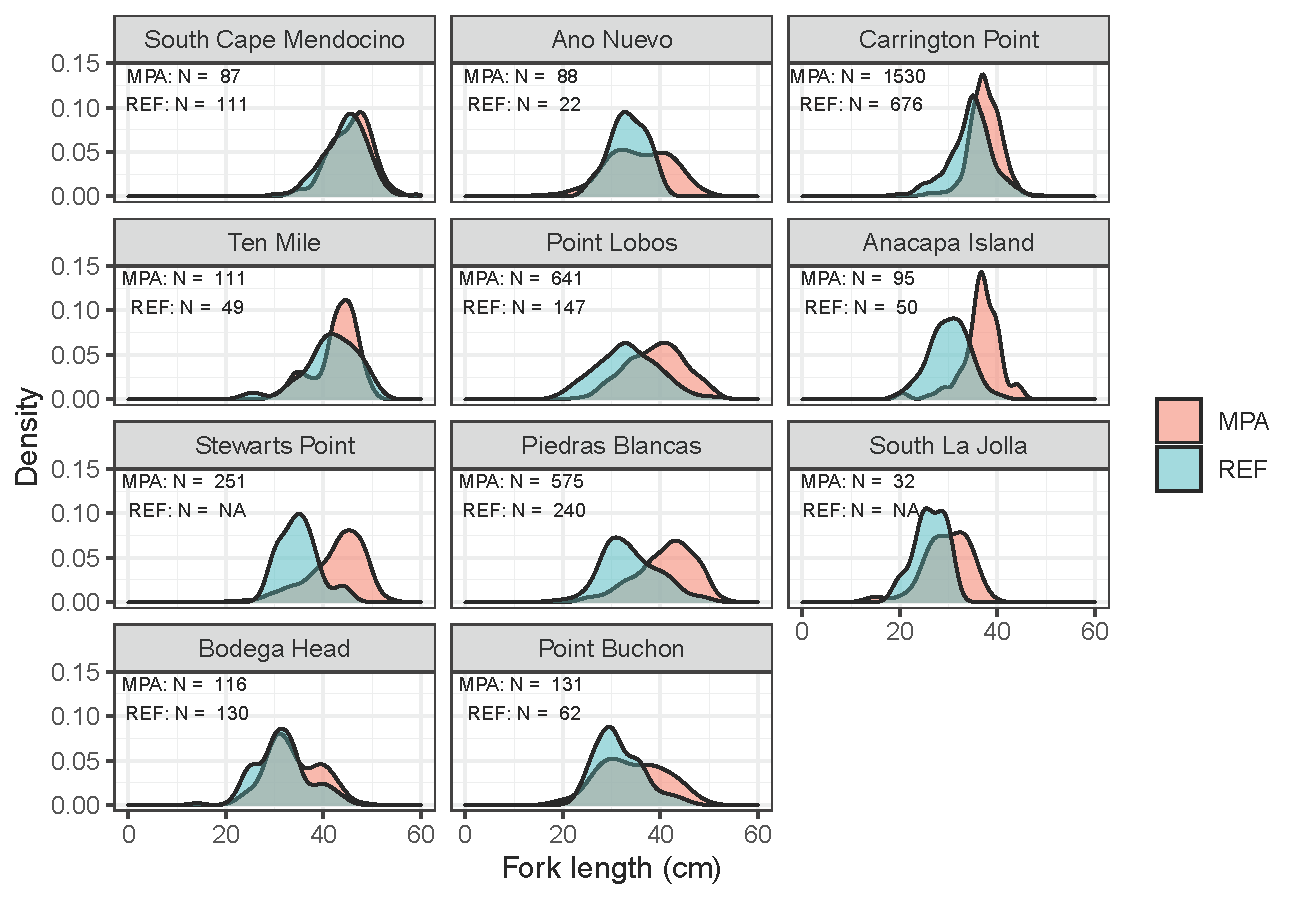
\includegraphics[width=1\textwidth,height=1\textheight]{C:/Assessments/2023/copper_rockfish_2023/docs/data_workshop/plots/ccfrp_copper_lengths.png}\\

\hypertarget{nwfsc-hook-and-line-survey-1}{%
\subsubsection{NWFSC Hook and Line
survey}\label{nwfsc-hook-and-line-survey-1}}

Between 2004-2021 the NWFSC Hook and Line survey has caught a total of
1,151 copper rockfish with otoliths for ageing being collected from each
fish. The majority of these observations have occurred outside the CCA
(outside CCA = 1,057 and inside CCA = 94). Observations of copper
rockfish have occurred across a range of depths between 22 - 66 fathoms
with the median of observations occurring around 44 fathoms. The NWFSC
Hook and Line data from 2022 is not yet available and not included in
these data summaries.

\begin{figure}
\centering
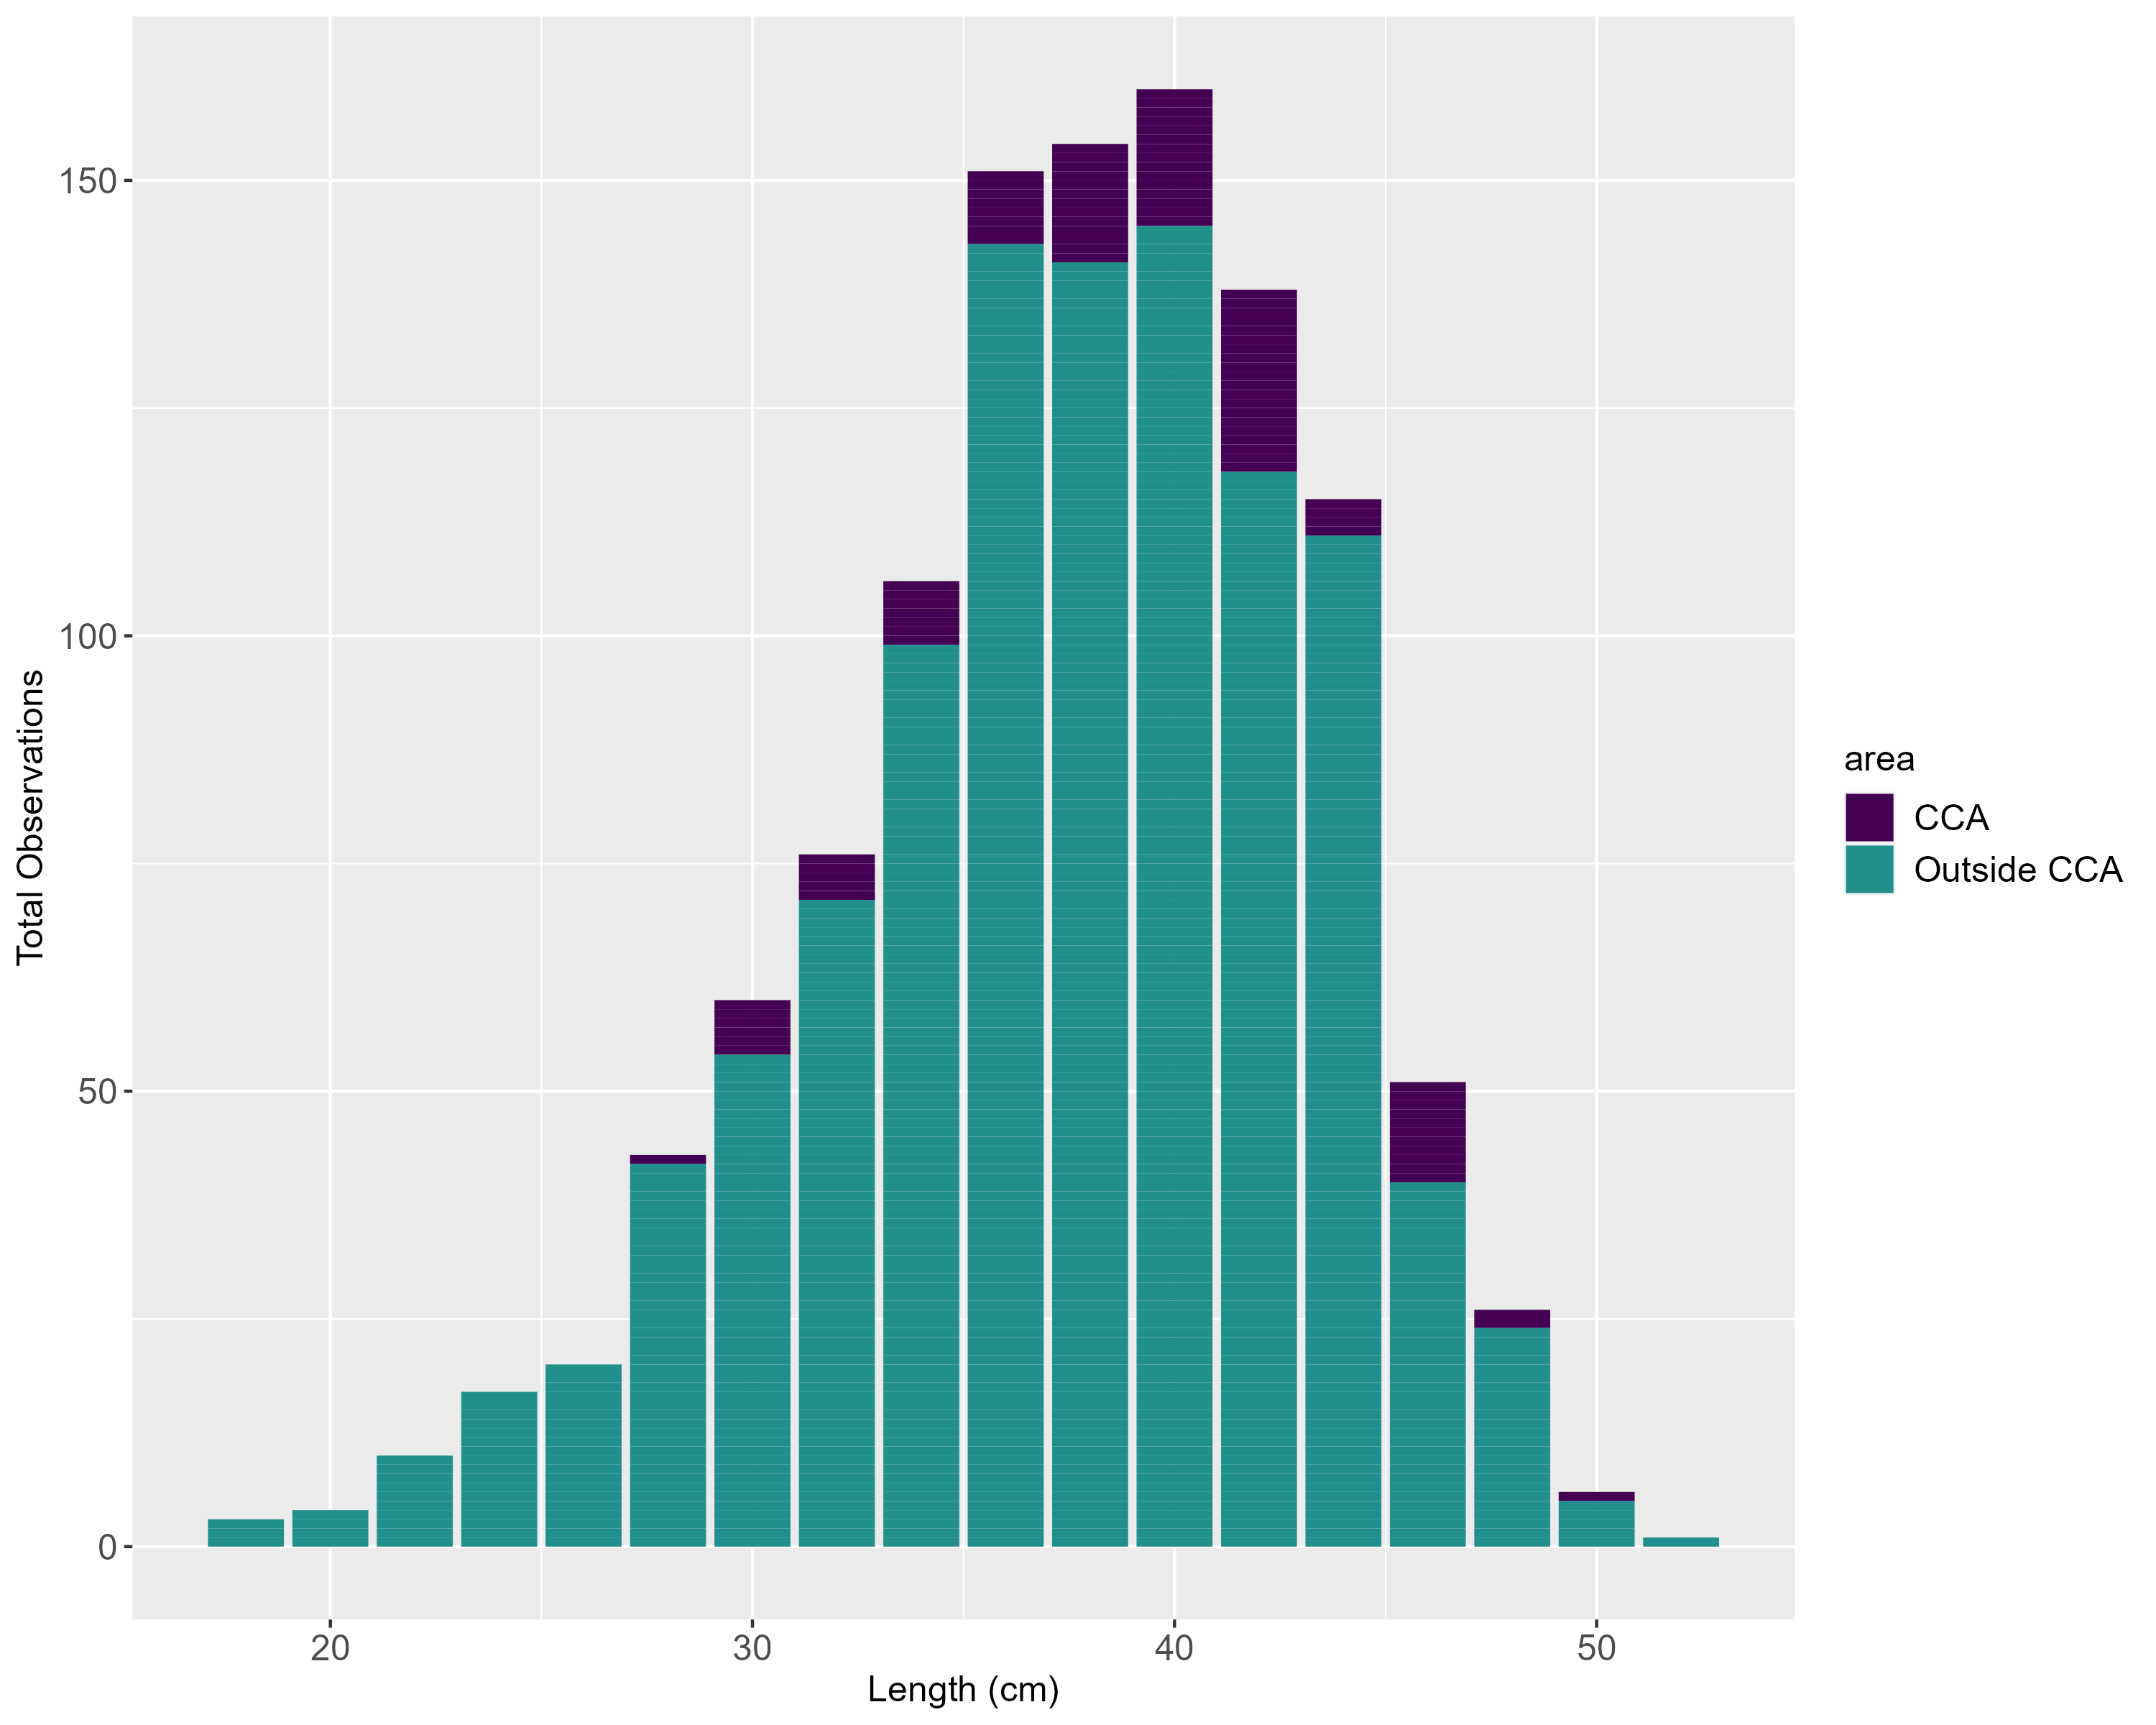
\includegraphics[width=1\textwidth,height=1\textheight]{C:/Assessments/2023/copper_rockfish_2023/docs/data_workshop/plots/hkl_observations_by_length_area.png}
\caption{Total observations by length (cm) of copper rockfish between
2004-2021 inside and outside of Cowcod Conservation Areas from the NWFSC
Hook and Line survey (source: NWFSC Hook and Line
survey).\label{fig:hkl-length-area}}
\end{figure}

\begin{figure}
\centering
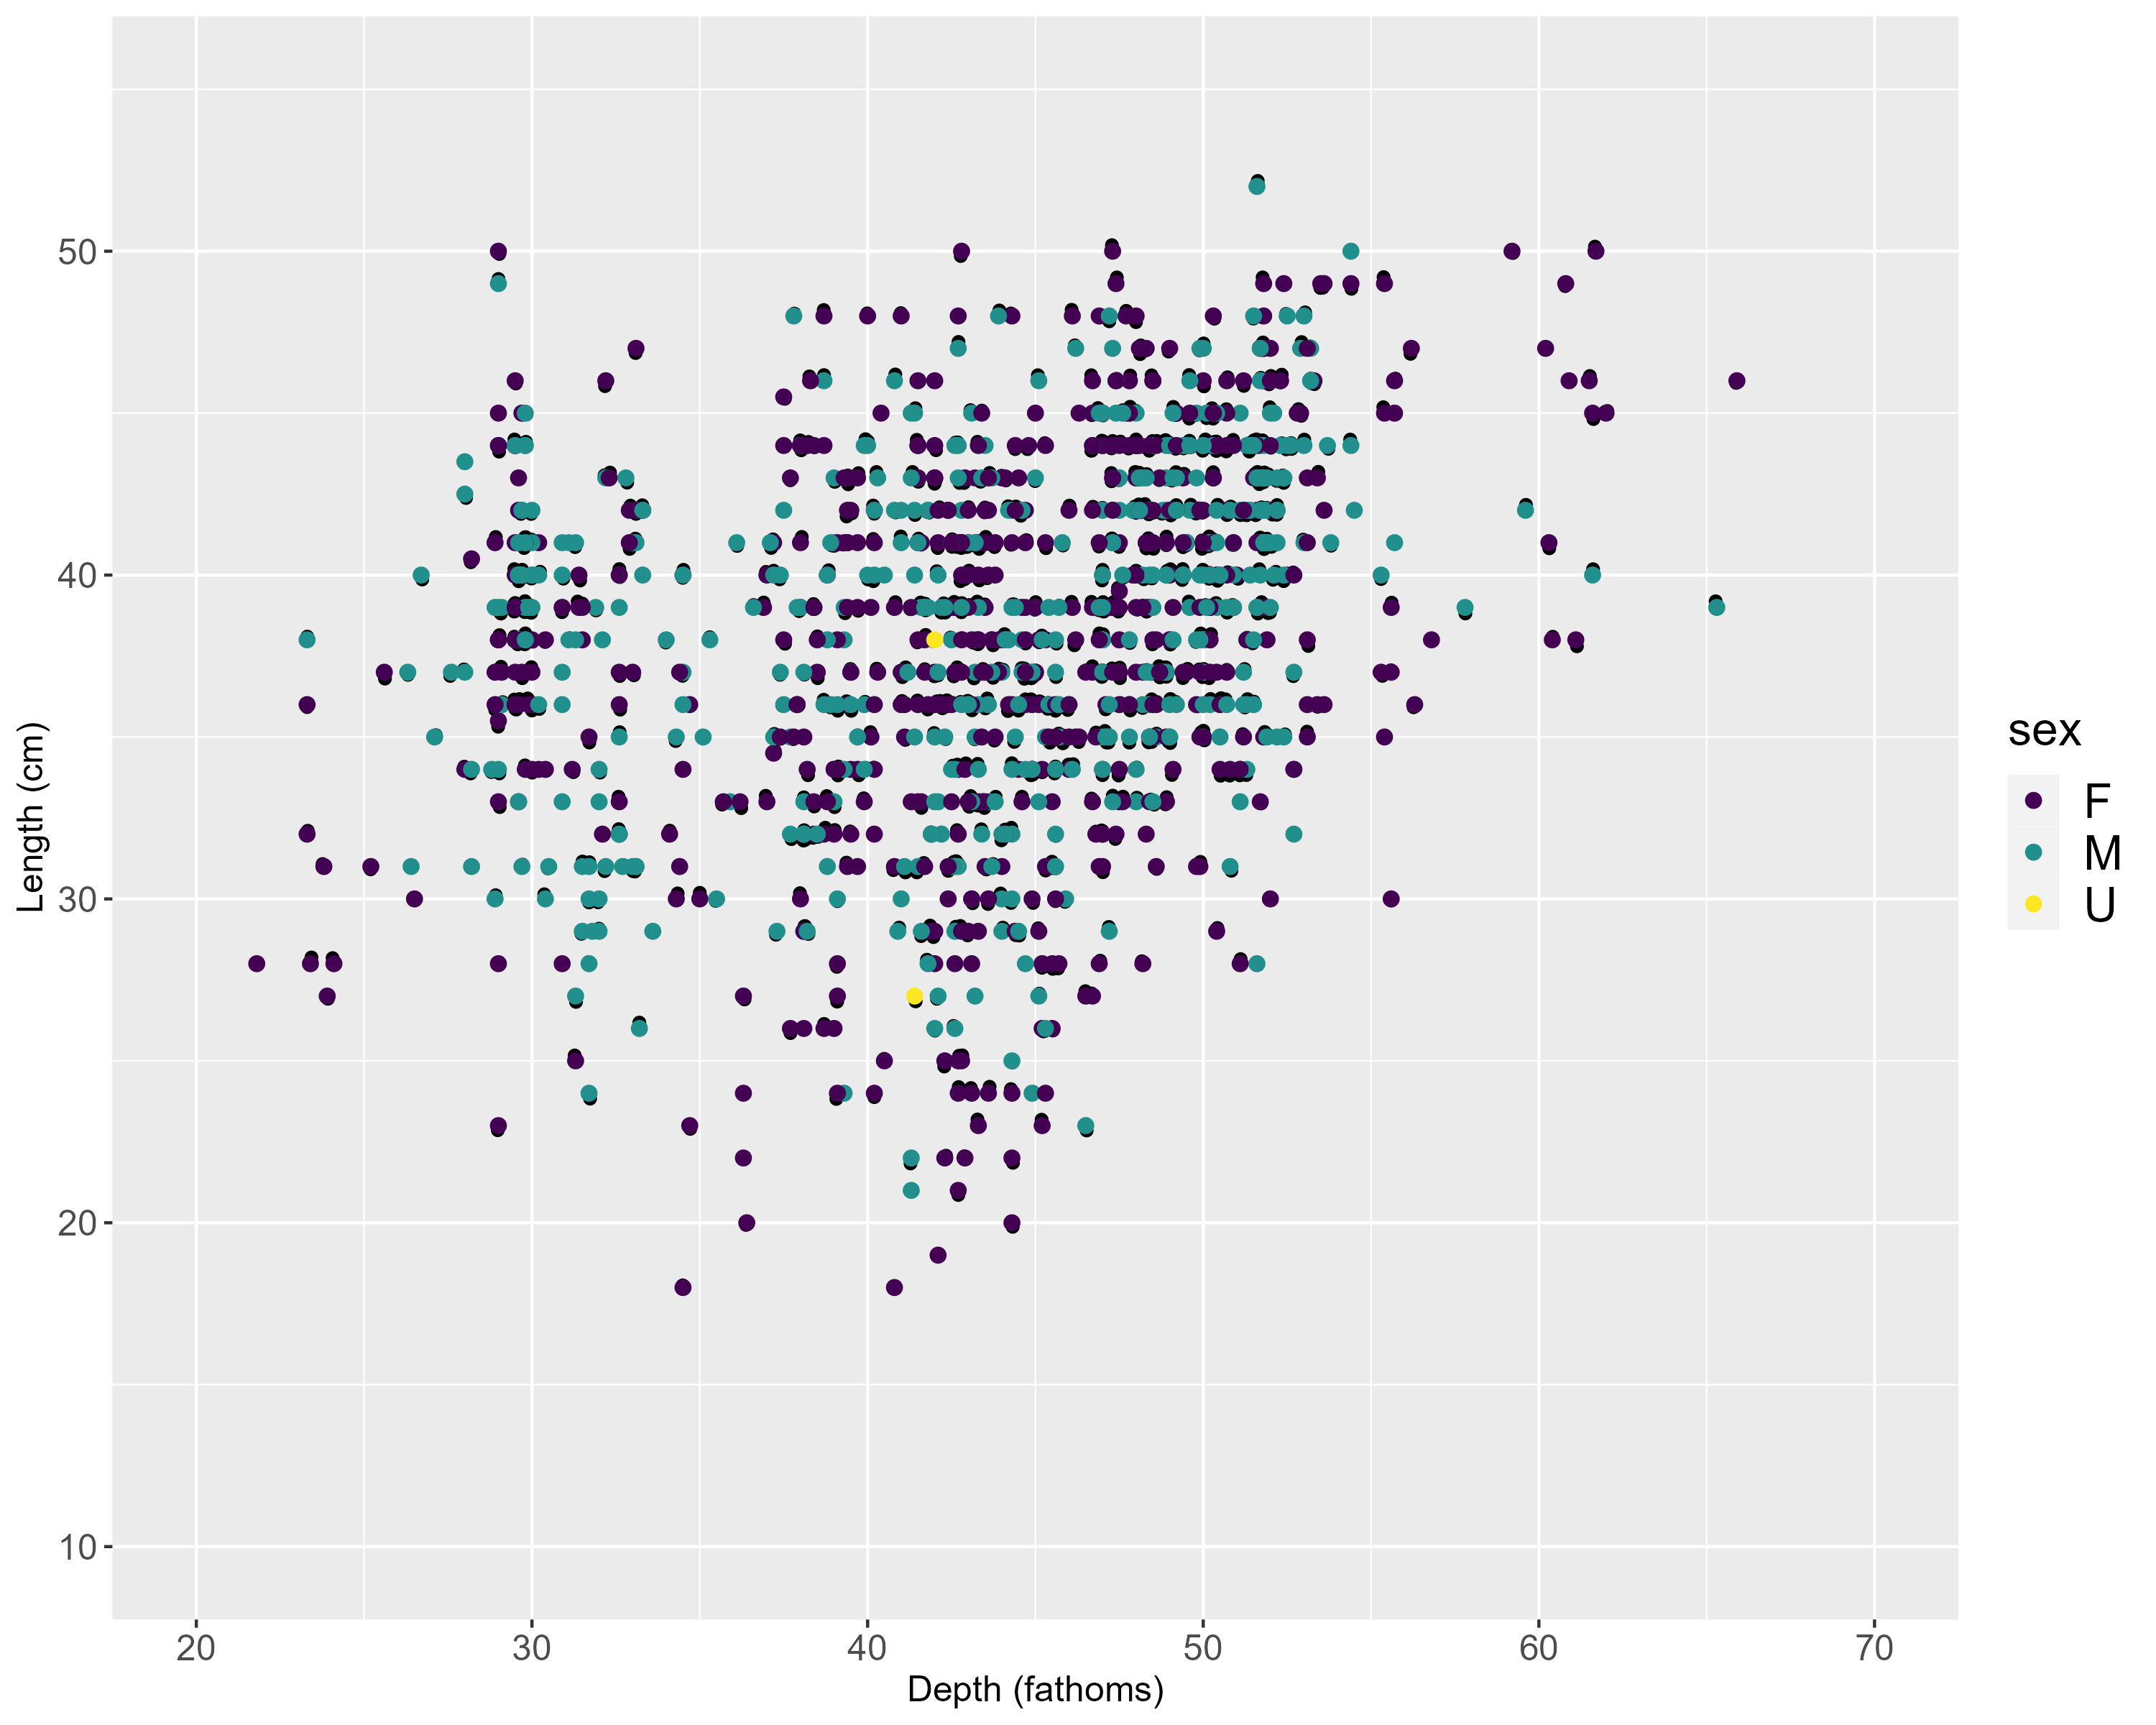
\includegraphics[width=1\textwidth,height=1\textheight]{C:/Assessments/2023/copper_rockfish_2023/docs/data_workshop/plots/hkl_length_sex_depth.png}
\caption{Measured lengths (cm) by depth in fathoms of copper rockfish
between 2004-2021 from the NWFSC Hook and Line survey (source: NWFSC
Hook and Line survey).\label{fig:hkl-length-depth}}
\end{figure}

\hypertarget{nwfsc-wcgbt-survey}{%
\subsubsection{NWFSC WCGBT survey}\label{nwfsc-wcgbt-survey}}

\begin{figure}
\centering
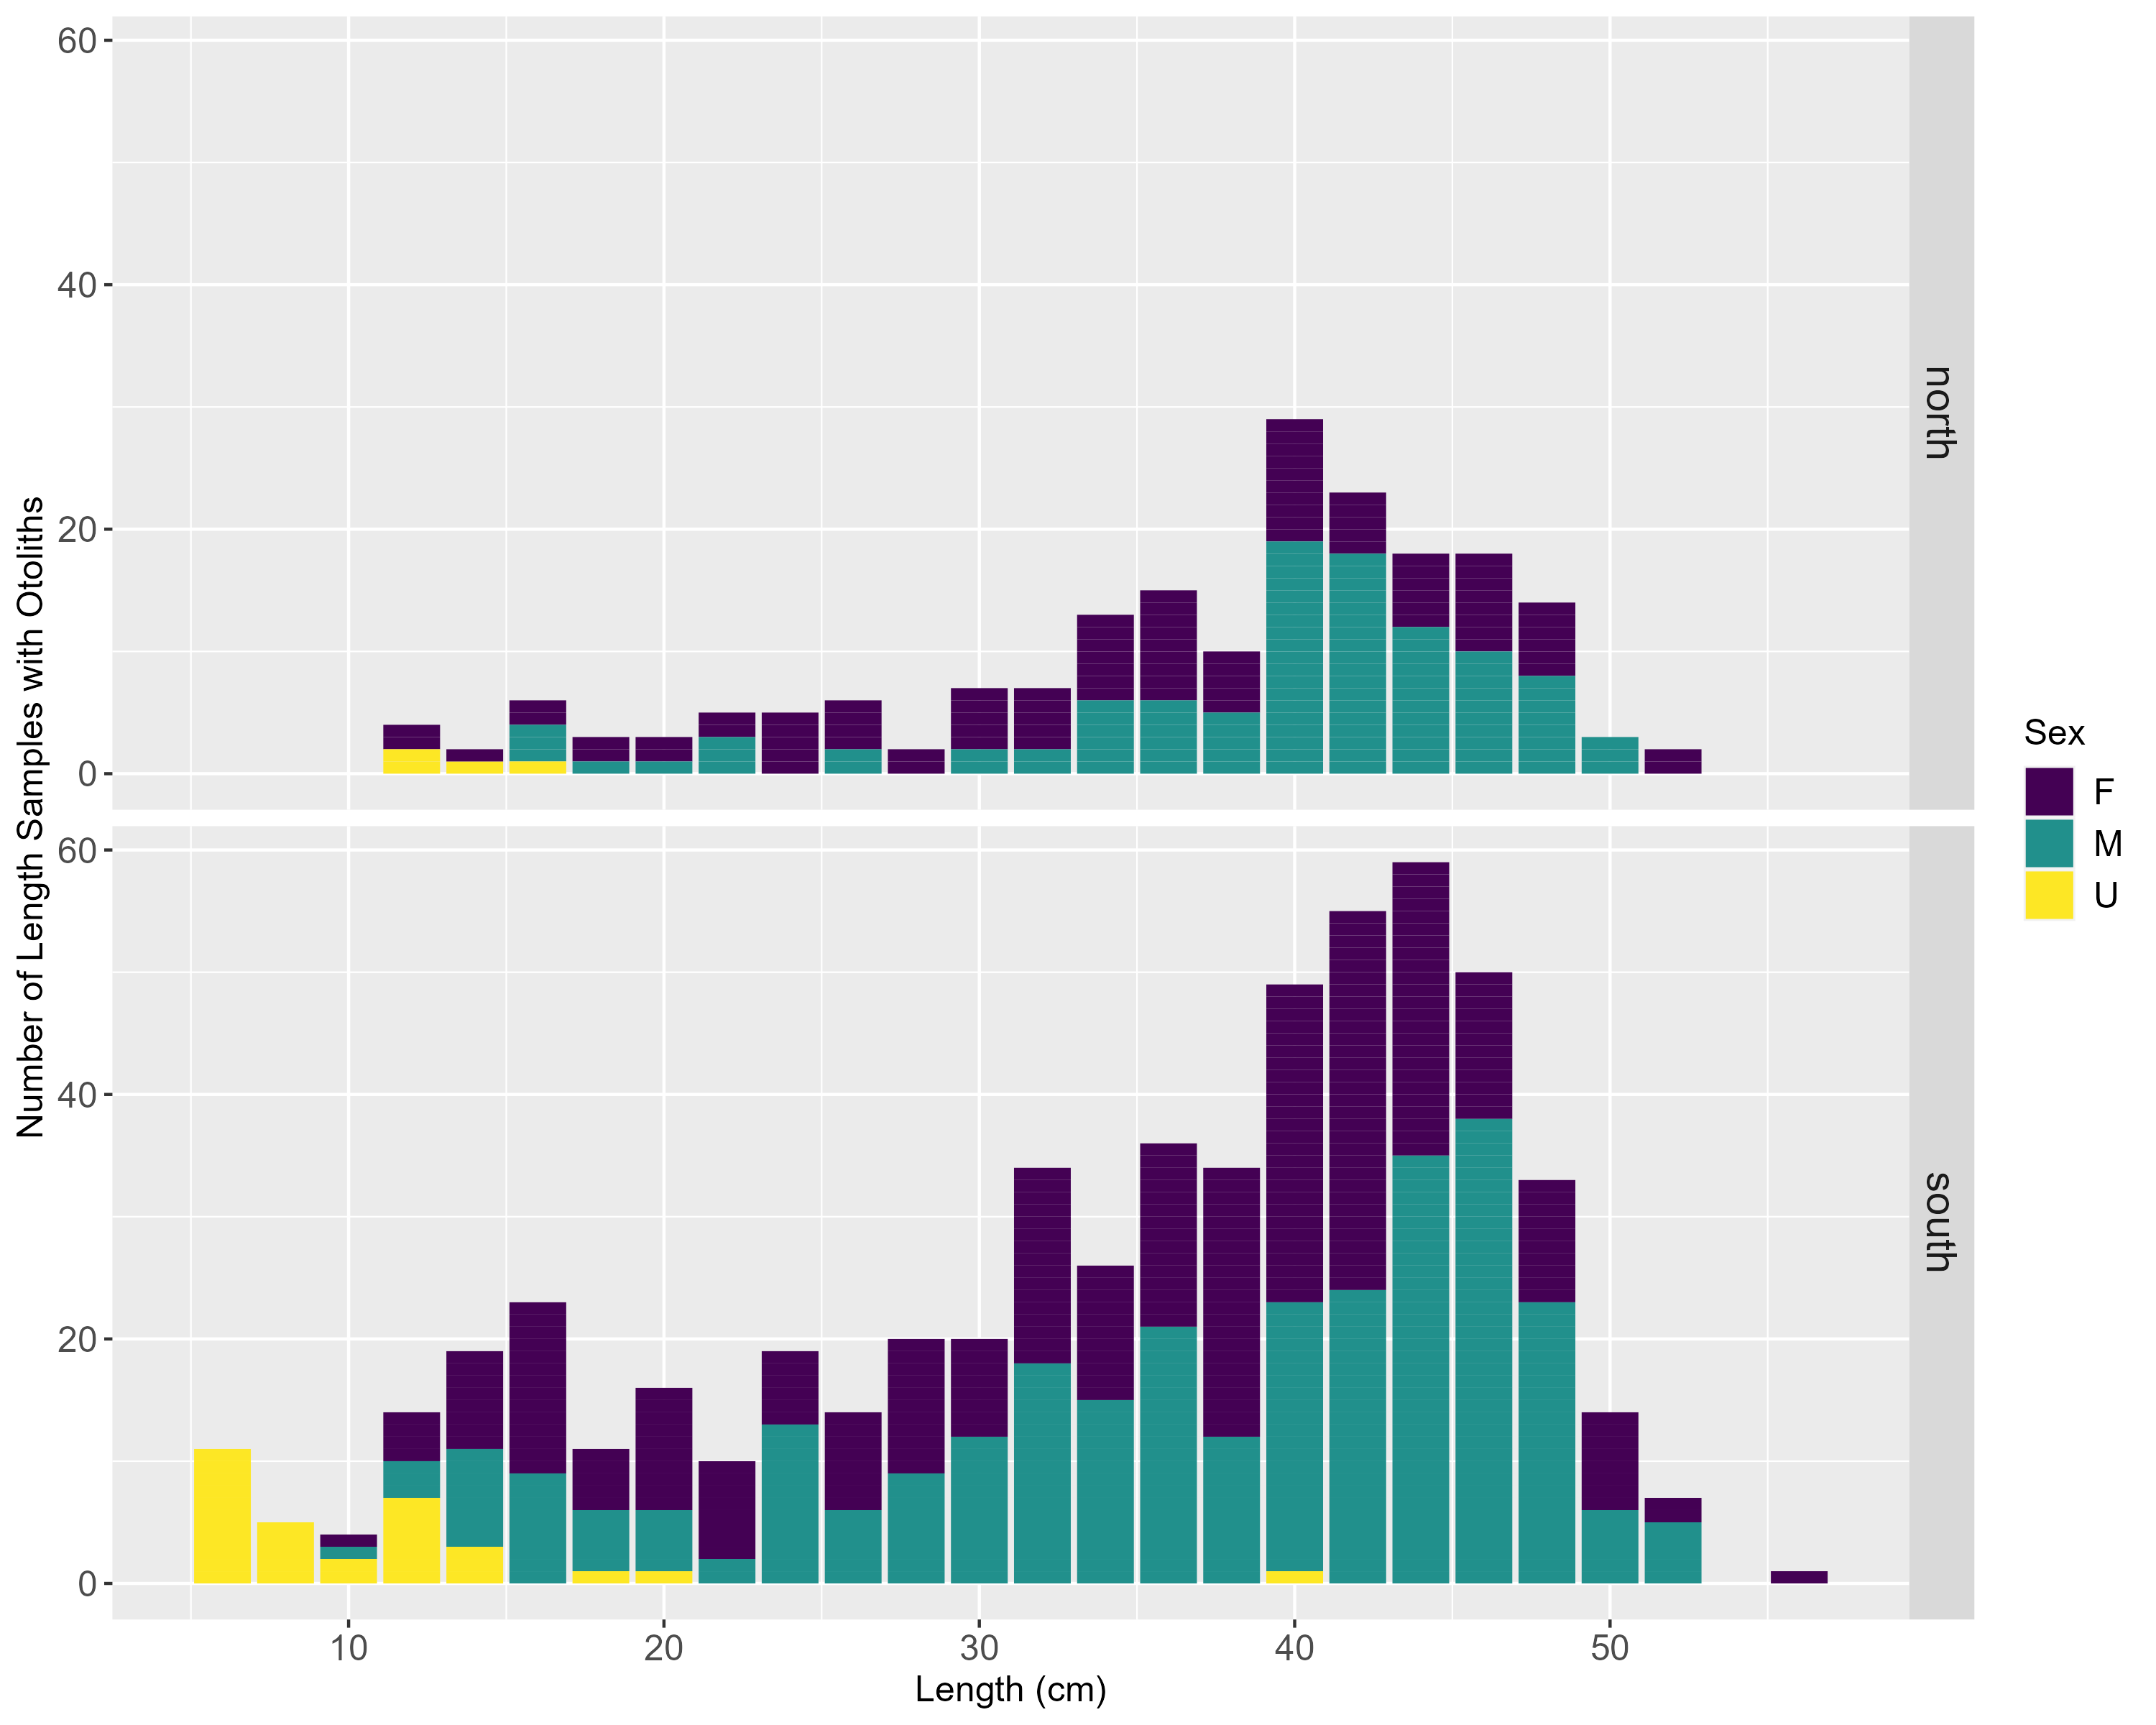
\includegraphics[width=1\textwidth,height=1\textheight]{C:/Assessments/2023/copper_rockfish_2023/docs/data_workshop/plots/wcgbt_length_samples_w_otoliths_by_area.png}
\caption{Number of lengths with otoliths by length and area collected by
the NWFSC WCGBT survey between 2003 - 2021. A total of 195 and 584
otoliths were collected from the areas north and south of Point
Conception, respectively (source: NWFSC WCGBT
survey).\label{fig:wcgbt-lengths}}
\end{figure}

\hypertarget{biology}{%
\section{Biology}\label{biology}}

\hypertarget{maturity-and-fecundity}{%
\subsection{Maturity and Fecundity}\label{maturity-and-fecundity}}

Currently, there is an extensive collaborative effort to collect
biological samples for copper rockfish in California. These samples will
support new estimates of maturity- and fecundity-at-length. These data
are not yet available but are expected to be completed in time for use
in the 2023 assessment of copper rockfish.

For informational purposes, maturity and fecundity curves that were used
in the 2021 assessment are shown below.

\begin{figure}
\centering
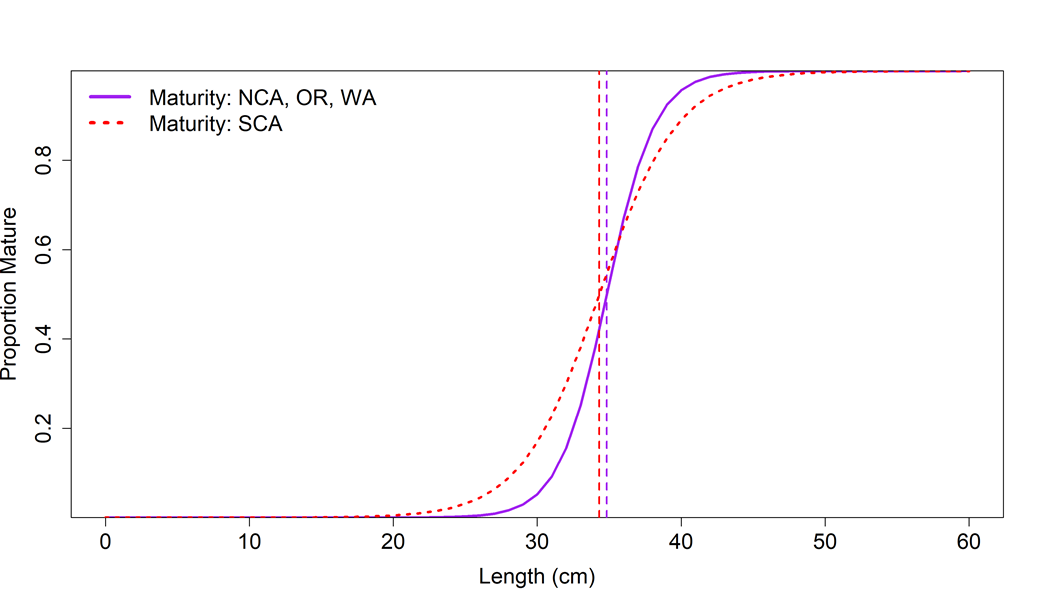
\includegraphics[width=1\textwidth,height=1\textheight]{C:/Assessments/2023/copper_rockfish_2023/docs/data_workshop/plots/maturity_2021.png}
\caption{Estimates of maturity-at-length used in the 2021 assessments of
copper rockfish. The same maturity curve was used in California north of
Point Conception, Oregon, and Washington. A unique maturity curve was
estimated based on 111 samples from the NWFSC WCGBT and Hook and Line
surveys south of Point Conception (source: Hannah, 2004; Melissa Head
(NWFSC)).\label{fig:maturity-2021}}
\end{figure}

\begin{figure}
\centering
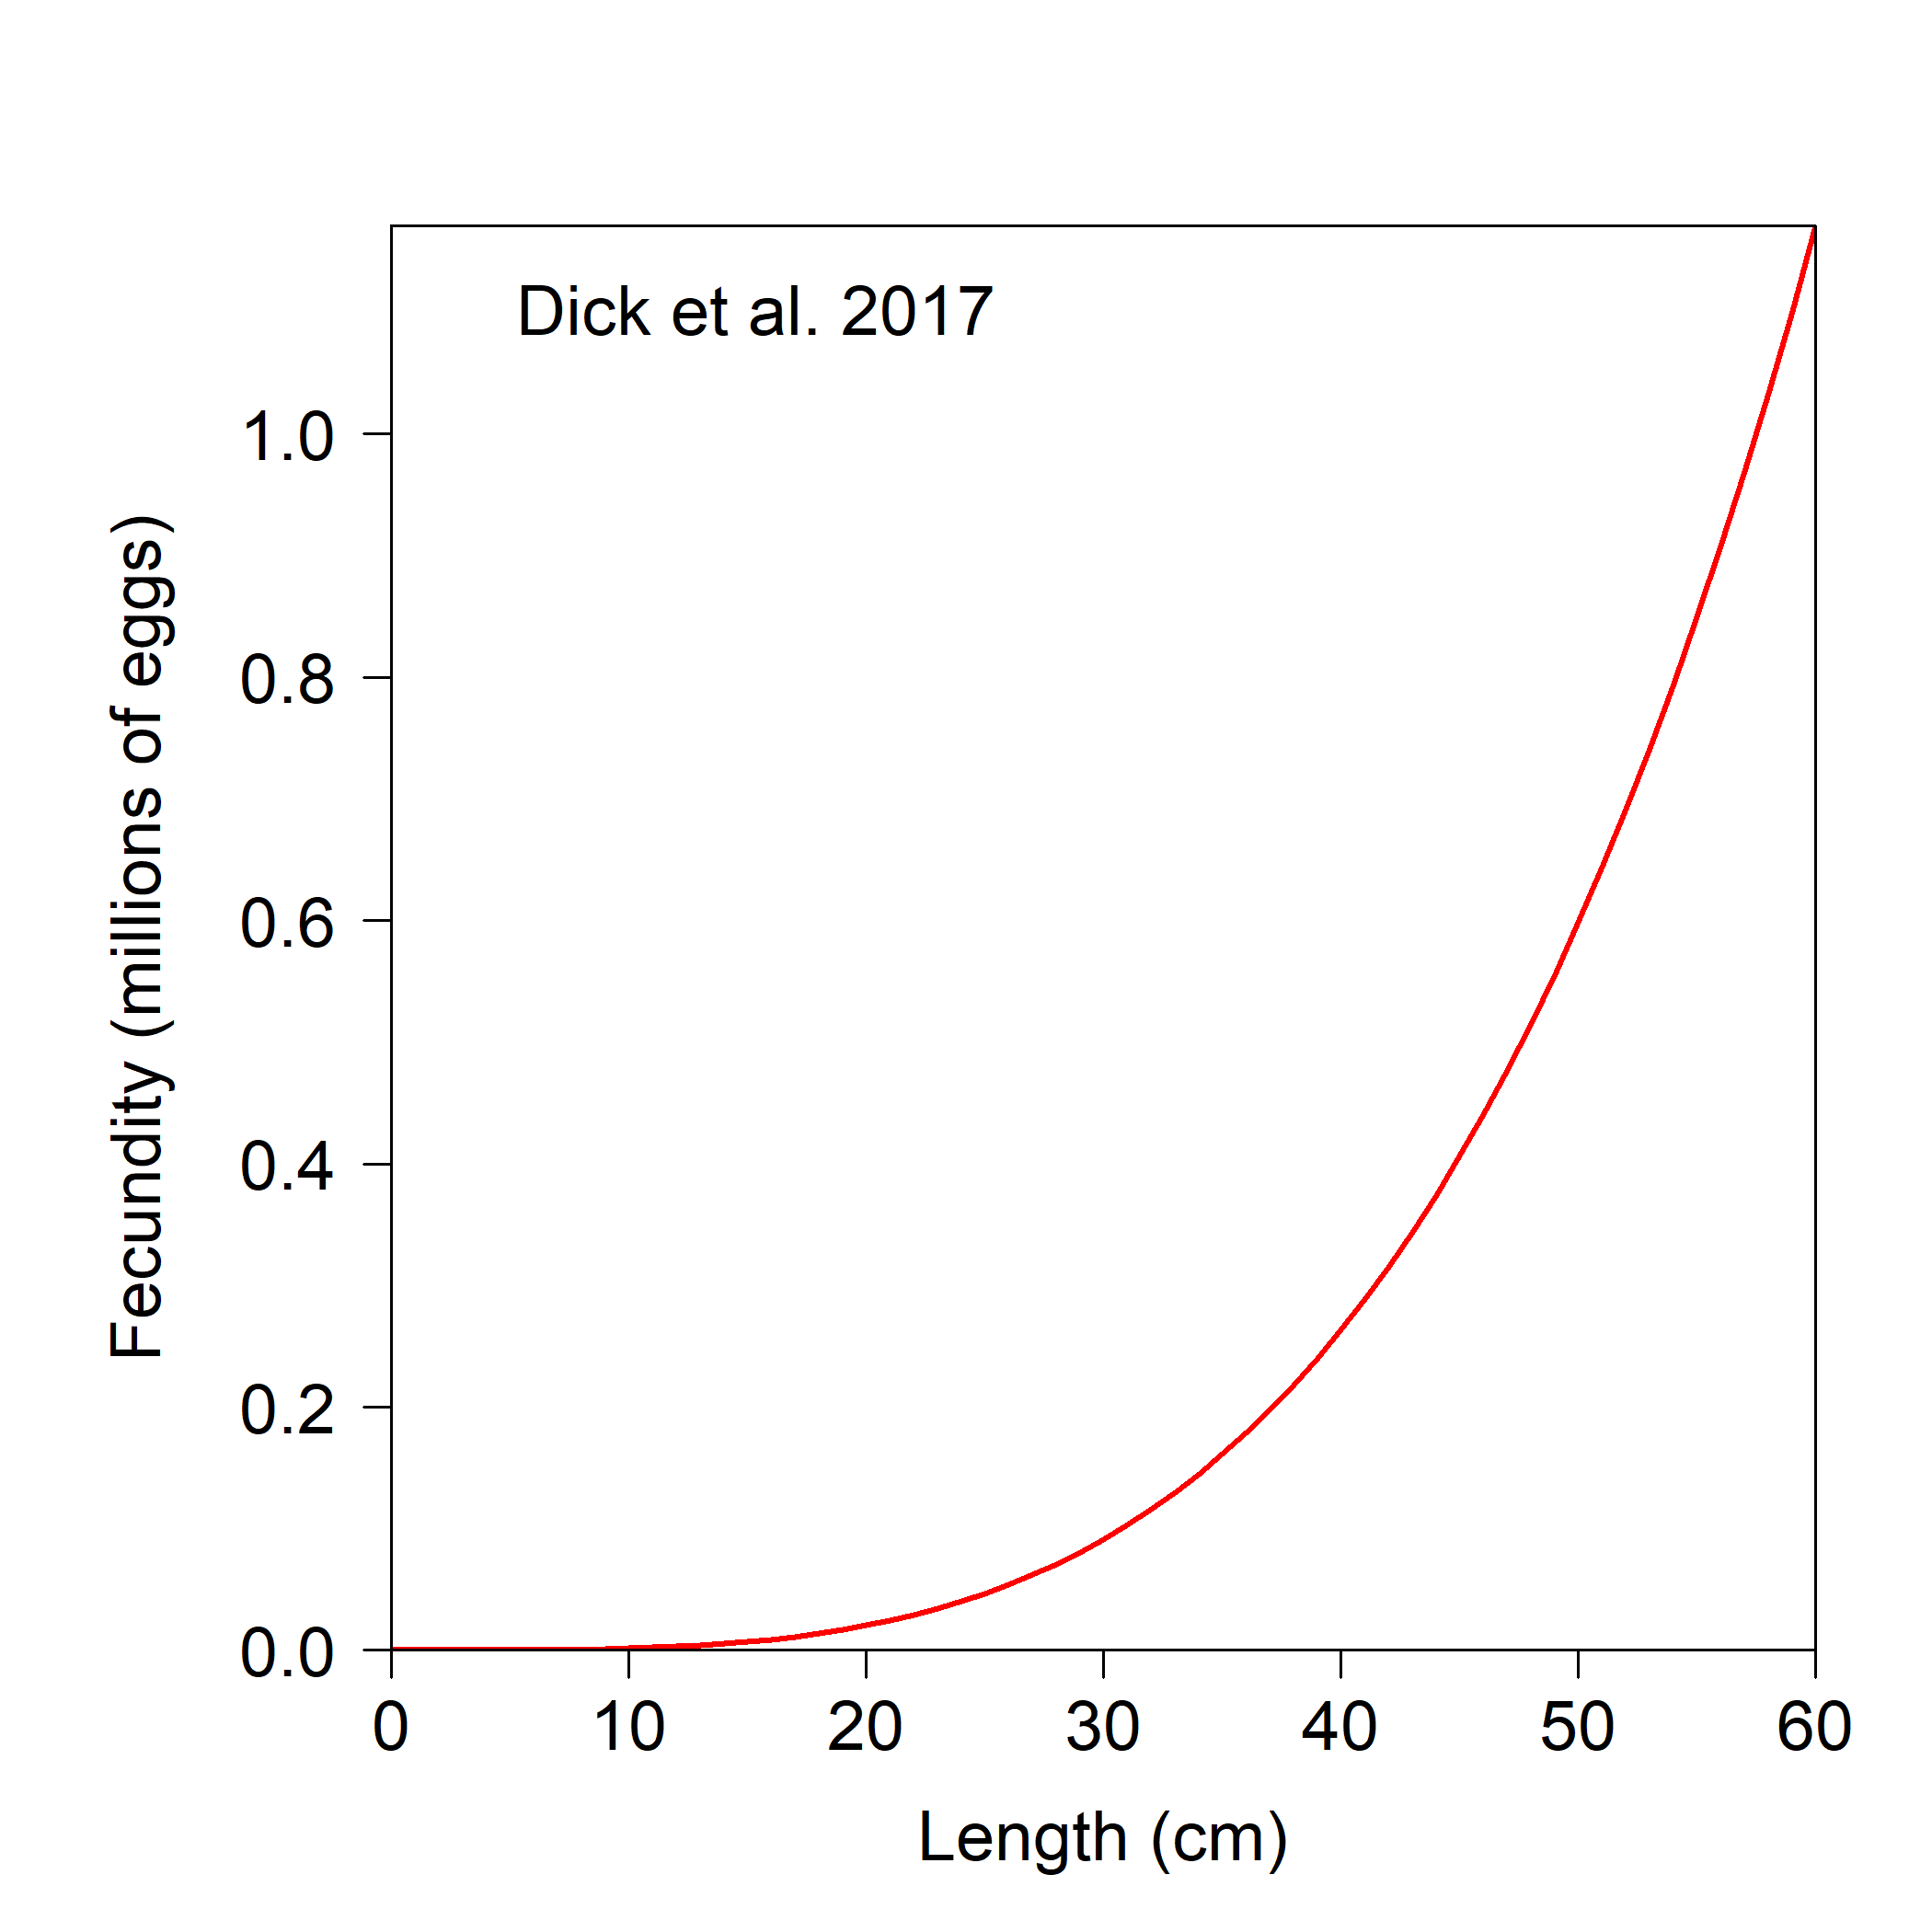
\includegraphics[width=0.75\textwidth,height=0.75\textheight]{C:/Assessments/2023/copper_rockfish_2023/docs/data_workshop/plots/Fecundity.png}
\caption{Estimates of fecundity-at-length used in the 2021 assessments
of copper rockfish. (source: Dick et al.,
2017).\label{fig:fecundity-2021}}
\end{figure}

\hypertarget{length-weight}{%
\subsection{Length-Weight}\label{length-weight}}

The length-weight relationship was estimated using all biological data
available from the NWFSC West Coast Groundfish Bottom Trawl (WCGBT) and
the NWFSC Hook and Line surveys.

\begin{figure}
\centering
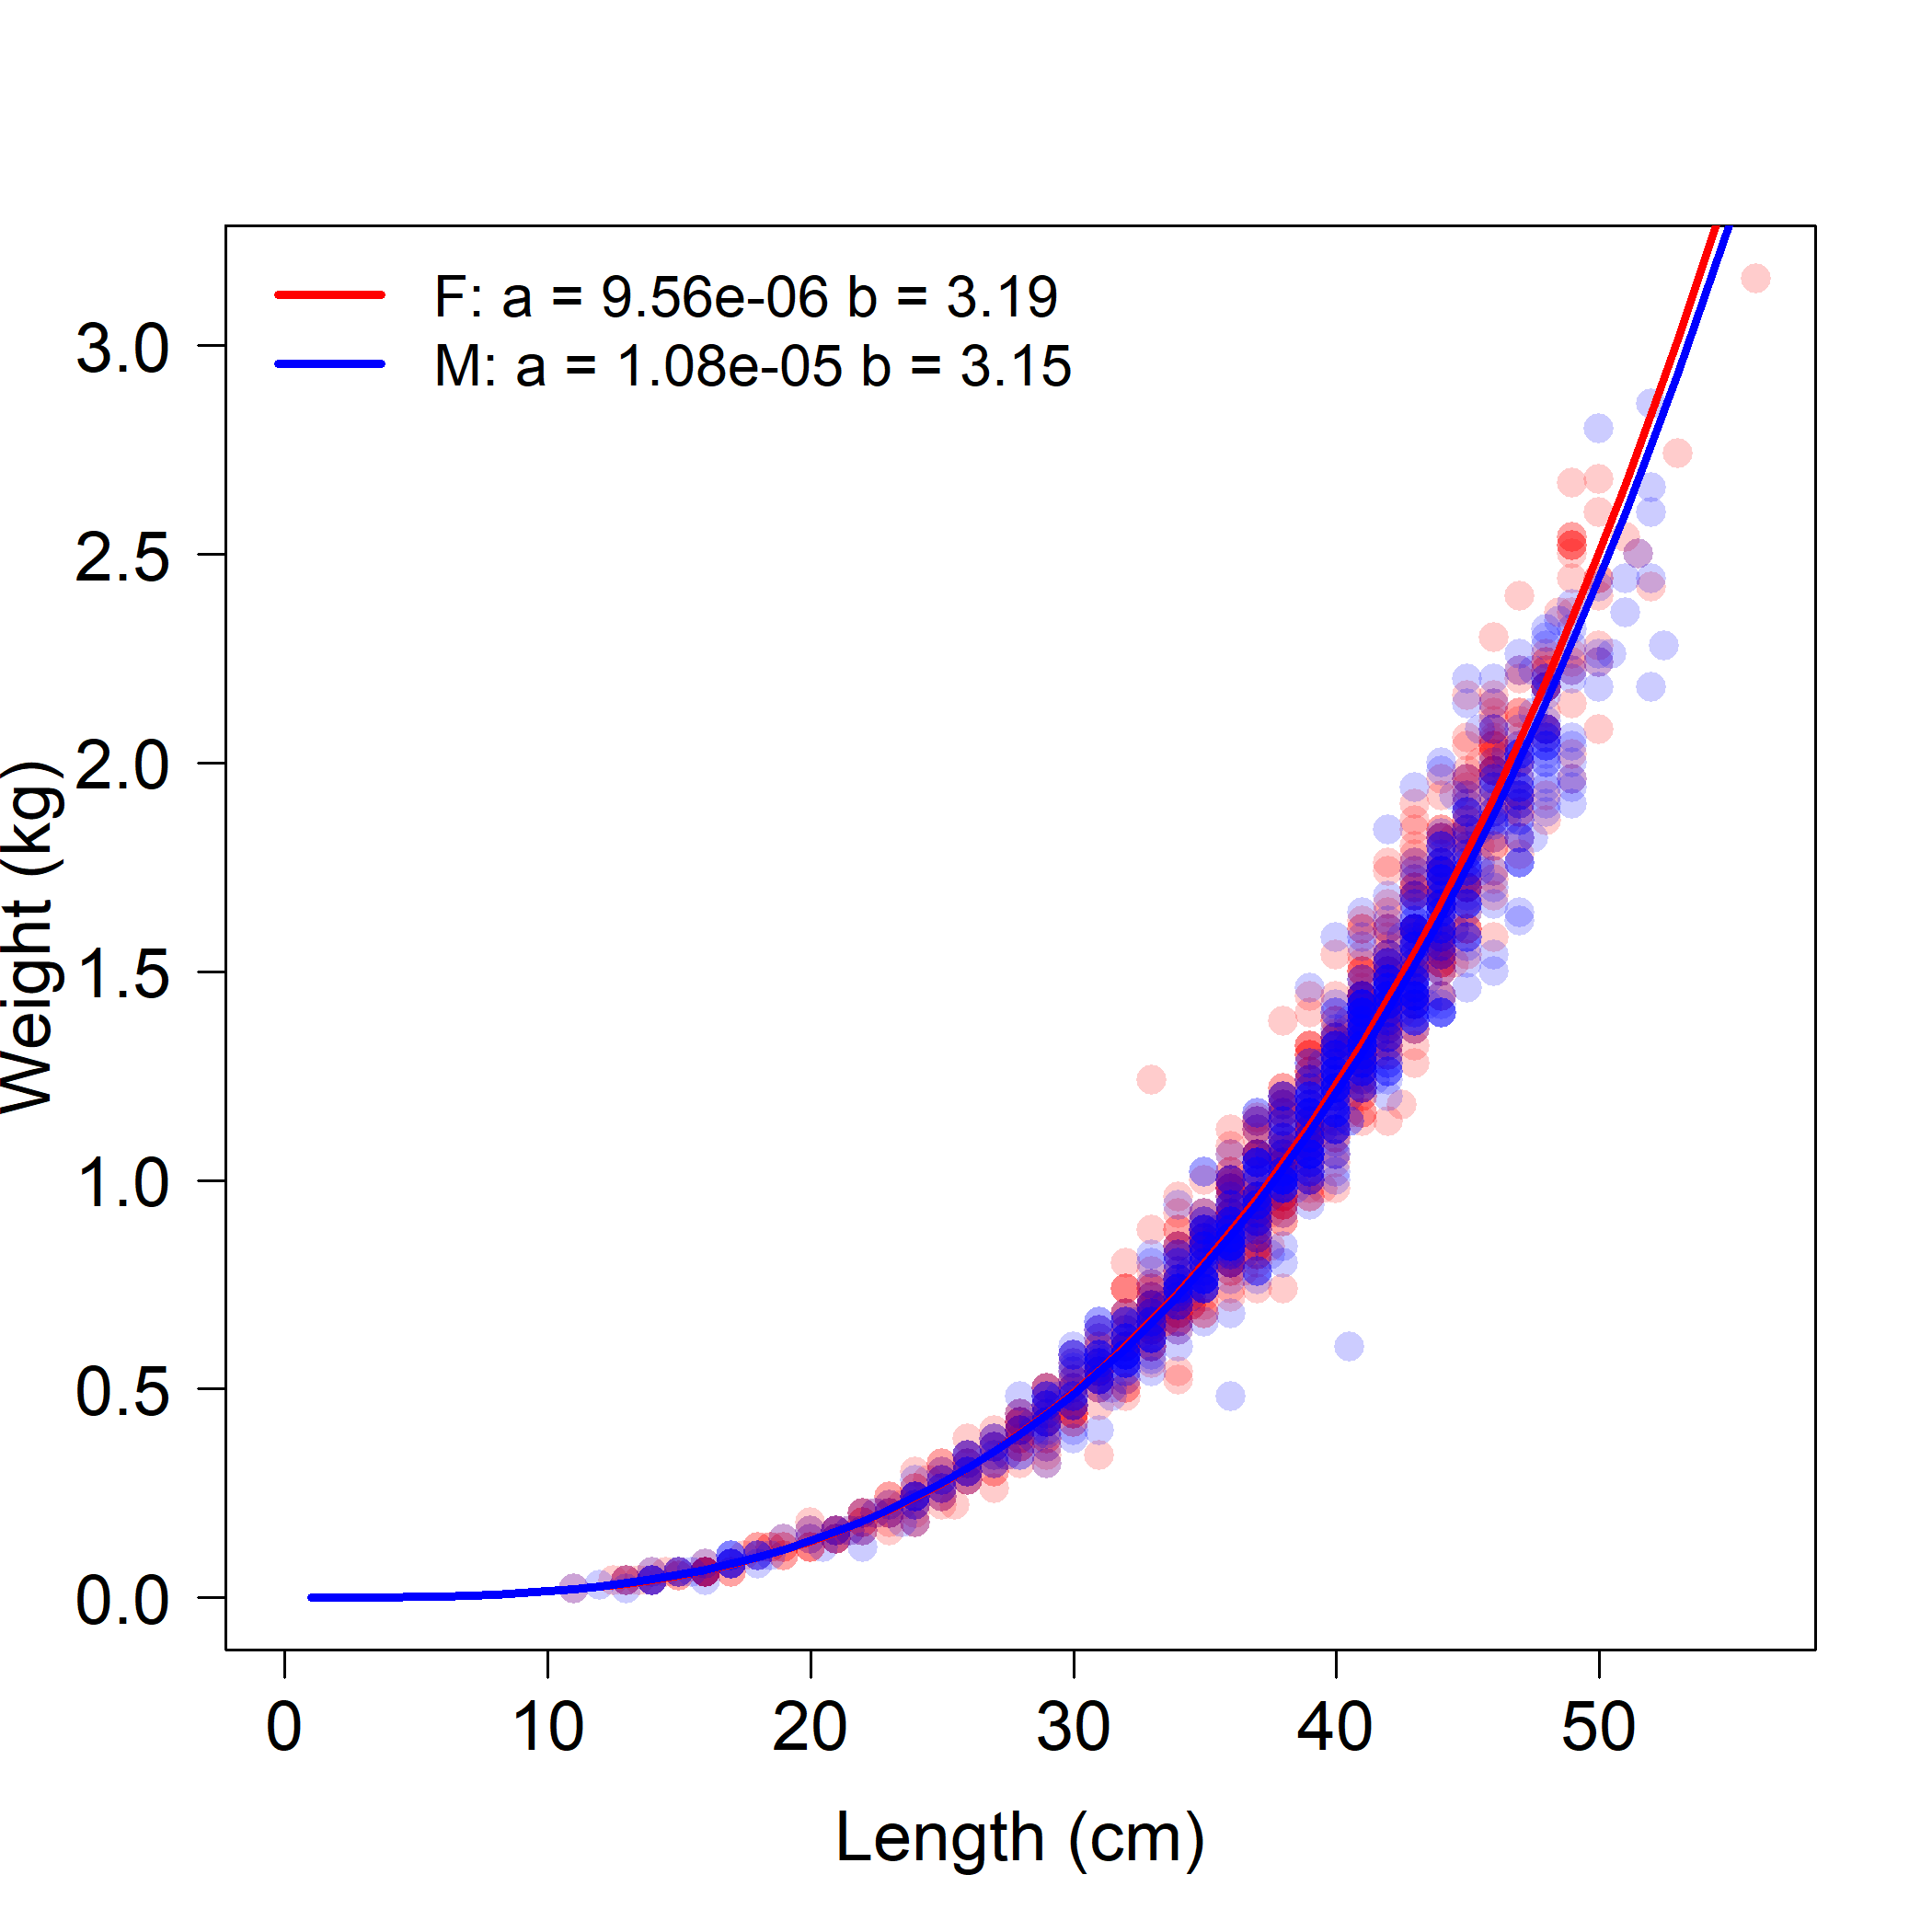
\includegraphics[width=0.75\textwidth,height=0.75\textheight]{C:/Assessments/2023/copper_rockfish_2023/docs/data_workshop/plots/doc_Length_Weight_Sex.png}
\caption{Estimated length-weight relationship by sex for copper rockfish
(source: NWFSC WCGBT and Hook and Line
Surveys).\label{fig:weight-length}}
\end{figure}

\hypertarget{length-at-age}{%
\subsection{Length-at-Age}\label{length-at-age}}

The NWFSC ageing lab is currently reading copper rockfish otoliths that
were not aged as part of the effort for the 2021 stock assessment. There
are a number of new sources of copper rockfish rockfish otoliths. The
below represent estimates of the number of copper rockfish ages expected
to be available for the 2023 assessment.

\begin{itemize}
\tightlist
\item
  North of Point Conception (N \textasciitilde{} 1,284):

  \begin{itemize}
  \tightlist
  \item
    211 from CPFV cooperative collections,
  \item
    99 from Private/Rental vessels collected by CDFW,
  \item
    79 from commercial fisheries,
  \item
    87 from CCFRP,
  \item
    423 from a research survey conducted by Don Pearson,
  \item
    195 from NWFSC WCGBT survey, and
  \item
    190 from historic data collections in the late-1970s and early 1980s
    (refugia) otoliths found by CDFW.
  \end{itemize}
\item
  South of Point Conception (N \textasciitilde{} 2,237):

  \begin{itemize}
  \tightlist
  \item
    484 from CPFV cooperative collections,
  \item
    9 from commercial fisheries,
  \item
    1,073+ from NWFSC hook and line survey,
  \item
    584 from NWFSC WCGBT survey,
  \item
    52 from CCFRP, and
  \item
    34 from a research survey conducted by Don Pearson.
  \end{itemize}
\item
  Otoliths that need to be linked to data north and south of Conception

  \begin{itemize}
  \tightlist
  \item
    304 from early recreational fisheries data collections from 1978,
    1981, and 1984
  \end{itemize}
\end{itemize}

\hypertarget{natural-mortality}{%
\subsection{Natural Mortality}\label{natural-mortality}}

Natural mortality was fixed in the 2021 assessments at a value of 0.108
yr\textsuperscript{-1} based on an assumed maximum age of 50 years. The
maximum age was selected based on available age data collected within
Oregon and Washington and literature values. The oldest aged observed
was 51 years with two observations off of the coast of Washington and
Oregon in 2019. This selection was consistent with the literature
examining the longevity of copper rockfish and was supported by the
observed ages that had multiple observations of fish between 44 and 51
years of age.

The input parameter value for natural mortality will be reconsidered
within the 2023 assessments based on any new available age data.
Additionally, the 2023 assessments will explore the ability to estimate
natural mortality within the model and will conduct sensitivities and
profiles to understand the information in the data on natural mortality
and the impact of select values on the model estimates.

\end{document}
